\documentclass[twoside]{book}

% Packages required by doxygen
\usepackage{fixltx2e}
\usepackage{calc}
\usepackage{doxygen}
\usepackage[export]{adjustbox} % also loads graphicx
\usepackage{graphicx}
\usepackage[utf8]{inputenc}
\usepackage{makeidx}
\usepackage{multicol}
\usepackage{multirow}
\PassOptionsToPackage{warn}{textcomp}
\usepackage{textcomp}
\usepackage[nointegrals]{wasysym}
\usepackage[table]{xcolor}

% Font selection
\usepackage[T1]{fontenc}
\usepackage[scaled=.90]{helvet}
\usepackage{courier}
\usepackage{amssymb}
\usepackage{sectsty}
\renewcommand{\familydefault}{\sfdefault}
\allsectionsfont{%
  \fontseries{bc}\selectfont%
  \color{darkgray}%
}
\renewcommand{\DoxyLabelFont}{%
  \fontseries{bc}\selectfont%
  \color{darkgray}%
}
\newcommand{\+}{\discretionary{\mbox{\scriptsize$\hookleftarrow$}}{}{}}

% Page & text layout
\usepackage{geometry}
\geometry{%
  a4paper,%
  top=2.5cm,%
  bottom=2.5cm,%
  left=2.5cm,%
  right=2.5cm%
}
\tolerance=750
\hfuzz=15pt
\hbadness=750
\setlength{\emergencystretch}{15pt}
\setlength{\parindent}{0cm}
\setlength{\parskip}{3ex plus 2ex minus 2ex}
\makeatletter
\renewcommand{\paragraph}{%
  \@startsection{paragraph}{4}{0ex}{-1.0ex}{1.0ex}{%
    \normalfont\normalsize\bfseries\SS@parafont%
  }%
}
\renewcommand{\subparagraph}{%
  \@startsection{subparagraph}{5}{0ex}{-1.0ex}{1.0ex}{%
    \normalfont\normalsize\bfseries\SS@subparafont%
  }%
}
\makeatother

% Headers & footers
\usepackage{fancyhdr}
\pagestyle{fancyplain}
\fancyhead[LE]{\fancyplain{}{\bfseries\thepage}}
\fancyhead[CE]{\fancyplain{}{}}
\fancyhead[RE]{\fancyplain{}{\bfseries\leftmark}}
\fancyhead[LO]{\fancyplain{}{\bfseries\rightmark}}
\fancyhead[CO]{\fancyplain{}{}}
\fancyhead[RO]{\fancyplain{}{\bfseries\thepage}}
\fancyfoot[LE]{\fancyplain{}{}}
\fancyfoot[CE]{\fancyplain{}{}}
\fancyfoot[RE]{\fancyplain{}{\bfseries\scriptsize Generated by Doxygen }}
\fancyfoot[LO]{\fancyplain{}{\bfseries\scriptsize Generated by Doxygen }}
\fancyfoot[CO]{\fancyplain{}{}}
\fancyfoot[RO]{\fancyplain{}{}}
\renewcommand{\footrulewidth}{0.4pt}
\renewcommand{\chaptermark}[1]{%
  \markboth{#1}{}%
}
\renewcommand{\sectionmark}[1]{%
  \markright{\thesection\ #1}%
}

% Indices & bibliography
\usepackage{natbib}
\usepackage[titles]{tocloft}
\setcounter{tocdepth}{3}
\setcounter{secnumdepth}{5}
\makeindex

% Hyperlinks (required, but should be loaded last)
\usepackage{ifpdf}
\ifpdf
  \usepackage[pdftex,pagebackref=true]{hyperref}
\else
  \usepackage[ps2pdf,pagebackref=true]{hyperref}
\fi
\hypersetup{%
  colorlinks=true,%
  linkcolor=blue,%
  citecolor=blue,%
  unicode%
}

% Custom commands
\newcommand{\clearemptydoublepage}{%
  \newpage{\pagestyle{empty}\cleardoublepage}%
}

\usepackage{caption}
\captionsetup{labelsep=space,justification=centering,font={bf},singlelinecheck=off,skip=4pt,position=top}

%===== C O N T E N T S =====

\begin{document}

% Titlepage & ToC
\hypersetup{pageanchor=false,
             bookmarksnumbered=true,
             pdfencoding=unicode
            }
\pagenumbering{roman}
\begin{titlepage}
\vspace*{7cm}
\begin{center}%
{\Large Stegosaurus \\[1ex]\large 1.\+0 }\\
\vspace*{1cm}
{\large Generated by Doxygen 1.8.11}\\
\end{center}
\end{titlepage}
\clearemptydoublepage
\tableofcontents
\clearemptydoublepage
\pagenumbering{arabic}
\hypersetup{pageanchor=true}

%--- Begin generated contents ---
\chapter{Namespace Index}
\section{Packages}
Here are the packages with brief descriptions (if available)\+:\begin{DoxyCompactList}
\item\contentsline{section}{\hyperlink{namespace_stegosaurus}{Stegosaurus} }{\pageref{namespace_stegosaurus}}{}
\item\contentsline{section}{\hyperlink{namespace_stegosaurus_1_1_algorithm}{Stegosaurus.\+Algorithm} }{\pageref{namespace_stegosaurus_1_1_algorithm}}{}
\item\contentsline{section}{\hyperlink{namespace_stegosaurus_1_1_algorithm_1_1_common_sample}{Stegosaurus.\+Algorithm.\+Common\+Sample} }{\pageref{namespace_stegosaurus_1_1_algorithm_1_1_common_sample}}{}
\item\contentsline{section}{\hyperlink{namespace_stegosaurus_1_1_algorithm_1_1_graph_theory}{Stegosaurus.\+Algorithm.\+Graph\+Theory} }{\pageref{namespace_stegosaurus_1_1_algorithm_1_1_graph_theory}}{}
\item\contentsline{section}{\hyperlink{namespace_stegosaurus_1_1_carrier}{Stegosaurus.\+Carrier} }{\pageref{namespace_stegosaurus_1_1_carrier}}{}
\item\contentsline{section}{\hyperlink{namespace_stegosaurus_1_1_carrier_1_1_audio_formats}{Stegosaurus.\+Carrier.\+Audio\+Formats} }{\pageref{namespace_stegosaurus_1_1_carrier_1_1_audio_formats}}{}
\item\contentsline{section}{\hyperlink{namespace_stegosaurus_1_1_cryptography}{Stegosaurus.\+Cryptography} }{\pageref{namespace_stegosaurus_1_1_cryptography}}{}
\item\contentsline{section}{\hyperlink{namespace_stegosaurus_1_1_exceptions}{Stegosaurus.\+Exceptions} }{\pageref{namespace_stegosaurus_1_1_exceptions}}{}
\item\contentsline{section}{\hyperlink{namespace_stegosaurus_1_1_extensions}{Stegosaurus.\+Extensions} }{\pageref{namespace_stegosaurus_1_1_extensions}}{}
\item\contentsline{section}{\hyperlink{namespace_stegosaurus_1_1_extensions_1_1_input_extensions}{Stegosaurus.\+Extensions.\+Input\+Extensions} }{\pageref{namespace_stegosaurus_1_1_extensions_1_1_input_extensions}}{}
\item\contentsline{section}{\hyperlink{namespace_stegosaurus_1_1_forms}{Stegosaurus.\+Forms} }{\pageref{namespace_stegosaurus_1_1_forms}}{}
\item\contentsline{section}{\hyperlink{namespace_stegosaurus_1_1_properties}{Stegosaurus.\+Properties} }{\pageref{namespace_stegosaurus_1_1_properties}}{}
\item\contentsline{section}{\hyperlink{namespace_stegosaurus_1_1_utility}{Stegosaurus.\+Utility} }{\pageref{namespace_stegosaurus_1_1_utility}}{}
\item\contentsline{section}{\hyperlink{namespace_stegosaurus_1_1_utility_1_1_extensions}{Stegosaurus.\+Utility.\+Extensions} }{\pageref{namespace_stegosaurus_1_1_utility_1_1_extensions}}{}
\item\contentsline{section}{\hyperlink{namespace_stegosaurus_1_1_utility_1_1_input_types}{Stegosaurus.\+Utility.\+Input\+Types} }{\pageref{namespace_stegosaurus_1_1_utility_1_1_input_types}}{}
\end{DoxyCompactList}

\chapter{Hierarchical Index}
\section{Class Hierarchy}
This inheritance list is sorted roughly, but not completely, alphabetically\+:\begin{DoxyCompactList}
\item \contentsline{section}{Stegosaurus.\+Carrier.\+Audio\+Formats.\+Audio\+File}{\pageref{class_stegosaurus_1_1_carrier_1_1_audio_formats_1_1_audio_file}}{}
\begin{DoxyCompactList}
\item \contentsline{section}{Stegosaurus.\+Carrier.\+Audio\+Formats.\+Wave\+File}{\pageref{class_stegosaurus_1_1_carrier_1_1_audio_formats_1_1_wave_file}}{}
\end{DoxyCompactList}
\item \contentsline{section}{Stegosaurus.\+Algorithm.\+Graph\+Theory.\+Counted\+Vertice\+List}{\pageref{class_stegosaurus_1_1_algorithm_1_1_graph_theory_1_1_counted_vertice_list}}{}
\item \contentsline{section}{Stegosaurus.\+Algorithm.\+Graph\+Theory.\+Edge}{\pageref{class_stegosaurus_1_1_algorithm_1_1_graph_theory_1_1_edge}}{}
\item Exception\begin{DoxyCompactList}
\item \contentsline{section}{Stegosaurus.\+Exceptions.\+Stegosaurus\+Exception}{\pageref{class_stegosaurus_1_1_exceptions_1_1_stegosaurus_exception}}{}
\begin{DoxyCompactList}
\item \contentsline{section}{Stegosaurus.\+Exceptions.\+Invalid\+Carrier\+File\+Exception}{\pageref{class_stegosaurus_1_1_exceptions_1_1_invalid_carrier_file_exception}}{}
\begin{DoxyCompactList}
\item \contentsline{section}{Stegosaurus.\+Exceptions.\+Invalid\+Image\+File\+Exception}{\pageref{class_stegosaurus_1_1_exceptions_1_1_invalid_image_file_exception}}{}
\item \contentsline{section}{Stegosaurus.\+Exceptions.\+Invalid\+Wave\+File\+Exception}{\pageref{class_stegosaurus_1_1_exceptions_1_1_invalid_wave_file_exception}}{}
\end{DoxyCompactList}
\item \contentsline{section}{Stegosaurus.\+Exceptions.\+Random\+Numbers\+Out\+Of\+Range\+Exception}{\pageref{class_stegosaurus_1_1_exceptions_1_1_random_numbers_out_of_range_exception}}{}
\item \contentsline{section}{Stegosaurus.\+Exceptions.\+Stego\+Algorithm\+Exception}{\pageref{class_stegosaurus_1_1_exceptions_1_1_stego_algorithm_exception}}{}
\item \contentsline{section}{Stegosaurus.\+Exceptions.\+Stego\+Crypto\+Exception}{\pageref{class_stegosaurus_1_1_exceptions_1_1_stego_crypto_exception}}{}
\item \contentsline{section}{Stegosaurus.\+Exceptions.\+Stego\+Message\+Exception}{\pageref{class_stegosaurus_1_1_exceptions_1_1_stego_message_exception}}{}
\end{DoxyCompactList}
\end{DoxyCompactList}
\item Form\begin{DoxyCompactList}
\item \contentsline{section}{Stegosaurus.\+Forms.\+Form\+Embedding\+Progress}{\pageref{class_stegosaurus_1_1_forms_1_1_form_embedding_progress}}{}
\item \contentsline{section}{Stegosaurus.\+Forms.\+Form\+Main}{\pageref{class_stegosaurus_1_1_forms_1_1_form_main}}{}
\end{DoxyCompactList}
\item \contentsline{section}{Stegosaurus.\+Carrier.\+I\+Carrier\+Media}{\pageref{interface_stegosaurus_1_1_carrier_1_1_i_carrier_media}}{}
\begin{DoxyCompactList}
\item \contentsline{section}{Stegosaurus.\+Carrier.\+Audio\+Carrier}{\pageref{class_stegosaurus_1_1_carrier_1_1_audio_carrier}}{}
\item \contentsline{section}{Stegosaurus.\+Carrier.\+Image\+Carrier}{\pageref{class_stegosaurus_1_1_carrier_1_1_image_carrier}}{}
\end{DoxyCompactList}
\item I\+Cloneable\begin{DoxyCompactList}
\item \contentsline{section}{Stegosaurus.\+Algorithm.\+Common\+Sample.\+Sample}{\pageref{class_stegosaurus_1_1_algorithm_1_1_common_sample_1_1_sample}}{}
\end{DoxyCompactList}
\item \contentsline{section}{Stegosaurus.\+Cryptography.\+I\+Crypto\+Provider}{\pageref{interface_stegosaurus_1_1_cryptography_1_1_i_crypto_provider}}{}
\begin{DoxyCompactList}
\item \contentsline{section}{Stegosaurus.\+Cryptography.\+A\+E\+S\+Provider}{\pageref{class_stegosaurus_1_1_cryptography_1_1_a_e_s_provider}}{}
\item \contentsline{section}{Stegosaurus.\+Cryptography.\+R\+S\+A\+Provider}{\pageref{class_stegosaurus_1_1_cryptography_1_1_r_s_a_provider}}{}
\item \contentsline{section}{Stegosaurus.\+Cryptography.\+Triple\+D\+E\+S\+Provider}{\pageref{class_stegosaurus_1_1_cryptography_1_1_triple_d_e_s_provider}}{}
\end{DoxyCompactList}
\item I\+Equatable\begin{DoxyCompactList}
\item \contentsline{section}{Stegosaurus.\+Algorithm.\+Common\+Sample.\+Sample}{\pageref{class_stegosaurus_1_1_algorithm_1_1_common_sample_1_1_sample}}{}
\end{DoxyCompactList}
\item \contentsline{section}{Stegosaurus.\+Utility.\+Input\+Types.\+I\+Input\+Type}{\pageref{interface_stegosaurus_1_1_utility_1_1_input_types_1_1_i_input_type}}{}
\begin{DoxyCompactList}
\item \contentsline{section}{Stegosaurus.\+Utility.\+Input\+Types.\+Carrier\+Type}{\pageref{class_stegosaurus_1_1_utility_1_1_input_types_1_1_carrier_type}}{}
\item \contentsline{section}{Stegosaurus.\+Utility.\+Input\+Types.\+Content\+Type}{\pageref{class_stegosaurus_1_1_utility_1_1_input_types_1_1_content_type}}{}
\end{DoxyCompactList}
\item \contentsline{section}{Stegosaurus.\+Extensions.\+Input\+Extensions.\+I\+Input\+Type}{\pageref{interface_stegosaurus_1_1_extensions_1_1_input_extensions_1_1_i_input_type}}{}
\begin{DoxyCompactList}
\item \contentsline{section}{Stegosaurus.\+Extensions.\+Input\+Extensions.\+Carrier\+Type}{\pageref{class_stegosaurus_1_1_extensions_1_1_input_extensions_1_1_carrier_type}}{}
\item \contentsline{section}{Stegosaurus.\+Extensions.\+Input\+Extensions.\+Content\+Type}{\pageref{class_stegosaurus_1_1_extensions_1_1_input_extensions_1_1_content_type}}{}
\end{DoxyCompactList}
\item \contentsline{section}{Stegosaurus.\+Input\+File}{\pageref{class_stegosaurus_1_1_input_file}}{}
\item \contentsline{section}{Stegosaurus.\+Utility.\+Random\+Number\+List}{\pageref{class_stegosaurus_1_1_utility_1_1_random_number_list}}{}
\item \contentsline{section}{Stegosaurus.\+Cryptography.\+R\+S\+A\+Key\+Pair}{\pageref{class_stegosaurus_1_1_cryptography_1_1_r_s_a_key_pair}}{}
\item \contentsline{section}{Stegosaurus.\+Algorithm.\+Graph\+Theory.\+Sample}{\pageref{class_stegosaurus_1_1_algorithm_1_1_graph_theory_1_1_sample}}{}
\item \contentsline{section}{Stegosaurus.\+Algorithm.\+Stego\+Algorithm\+Base}{\pageref{class_stegosaurus_1_1_algorithm_1_1_stego_algorithm_base}}{}
\begin{DoxyCompactList}
\item \contentsline{section}{Stegosaurus.\+Algorithm.\+Common\+Sample\+Algorithm}{\pageref{class_stegosaurus_1_1_algorithm_1_1_common_sample_algorithm}}{}
\item \contentsline{section}{Stegosaurus.\+Algorithm.\+Graph\+Theoretic\+Algorithm}{\pageref{class_stegosaurus_1_1_algorithm_1_1_graph_theoretic_algorithm}}{}
\item \contentsline{section}{Stegosaurus.\+Algorithm.\+L\+S\+B\+Algorithm}{\pageref{class_stegosaurus_1_1_algorithm_1_1_l_s_b_algorithm}}{}
\end{DoxyCompactList}
\item \contentsline{section}{Stegosaurus.\+Stego\+Message}{\pageref{class_stegosaurus_1_1_stego_message}}{}
\item \contentsline{section}{Stegosaurus.\+Algorithm.\+Graph\+Theory.\+Vertex}{\pageref{class_stegosaurus_1_1_algorithm_1_1_graph_theory_1_1_vertex}}{}
\end{DoxyCompactList}

\chapter{Class Index}
\section{Class List}
Here are the classes, structs, unions and interfaces with brief descriptions\+:\begin{DoxyCompactList}
\item\contentsline{section}{\hyperlink{class_stegosaurus_1_1_cryptography_1_1_a_e_s_provider}{Stegosaurus.\+Cryptography.\+A\+E\+S\+Provider} }{\pageref{class_stegosaurus_1_1_cryptography_1_1_a_e_s_provider}}{}
\item\contentsline{section}{\hyperlink{class_stegosaurus_1_1_carrier_1_1_audio_carrier}{Stegosaurus.\+Carrier.\+Audio\+Carrier} }{\pageref{class_stegosaurus_1_1_carrier_1_1_audio_carrier}}{}
\item\contentsline{section}{\hyperlink{class_stegosaurus_1_1_carrier_1_1_audio_formats_1_1_audio_file}{Stegosaurus.\+Carrier.\+Audio\+Formats.\+Audio\+File} }{\pageref{class_stegosaurus_1_1_carrier_1_1_audio_formats_1_1_audio_file}}{}
\item\contentsline{section}{\hyperlink{class_stegosaurus_1_1_utility_1_1_input_types_1_1_carrier_type}{Stegosaurus.\+Utility.\+Input\+Types.\+Carrier\+Type} }{\pageref{class_stegosaurus_1_1_utility_1_1_input_types_1_1_carrier_type}}{}
\item\contentsline{section}{\hyperlink{class_stegosaurus_1_1_extensions_1_1_input_extensions_1_1_carrier_type}{Stegosaurus.\+Extensions.\+Input\+Extensions.\+Carrier\+Type} }{\pageref{class_stegosaurus_1_1_extensions_1_1_input_extensions_1_1_carrier_type}}{}
\item\contentsline{section}{\hyperlink{class_stegosaurus_1_1_algorithm_1_1_common_sample_algorithm}{Stegosaurus.\+Algorithm.\+Common\+Sample\+Algorithm} }{\pageref{class_stegosaurus_1_1_algorithm_1_1_common_sample_algorithm}}{}
\item\contentsline{section}{\hyperlink{class_stegosaurus_1_1_utility_1_1_input_types_1_1_content_type}{Stegosaurus.\+Utility.\+Input\+Types.\+Content\+Type} }{\pageref{class_stegosaurus_1_1_utility_1_1_input_types_1_1_content_type}}{}
\item\contentsline{section}{\hyperlink{class_stegosaurus_1_1_extensions_1_1_input_extensions_1_1_content_type}{Stegosaurus.\+Extensions.\+Input\+Extensions.\+Content\+Type} }{\pageref{class_stegosaurus_1_1_extensions_1_1_input_extensions_1_1_content_type}}{}
\item\contentsline{section}{\hyperlink{class_stegosaurus_1_1_algorithm_1_1_graph_theory_1_1_counted_vertice_list}{Stegosaurus.\+Algorithm.\+Graph\+Theory.\+Counted\+Vertice\+List} }{\pageref{class_stegosaurus_1_1_algorithm_1_1_graph_theory_1_1_counted_vertice_list}}{}
\item\contentsline{section}{\hyperlink{class_stegosaurus_1_1_algorithm_1_1_graph_theory_1_1_edge}{Stegosaurus.\+Algorithm.\+Graph\+Theory.\+Edge} }{\pageref{class_stegosaurus_1_1_algorithm_1_1_graph_theory_1_1_edge}}{}
\item\contentsline{section}{\hyperlink{class_stegosaurus_1_1_forms_1_1_form_embedding_progress}{Stegosaurus.\+Forms.\+Form\+Embedding\+Progress} }{\pageref{class_stegosaurus_1_1_forms_1_1_form_embedding_progress}}{}
\item\contentsline{section}{\hyperlink{class_stegosaurus_1_1_forms_1_1_form_main}{Stegosaurus.\+Forms.\+Form\+Main} }{\pageref{class_stegosaurus_1_1_forms_1_1_form_main}}{}
\item\contentsline{section}{\hyperlink{class_stegosaurus_1_1_algorithm_1_1_graph_theoretic_algorithm}{Stegosaurus.\+Algorithm.\+Graph\+Theoretic\+Algorithm} }{\pageref{class_stegosaurus_1_1_algorithm_1_1_graph_theoretic_algorithm}}{}
\item\contentsline{section}{\hyperlink{interface_stegosaurus_1_1_carrier_1_1_i_carrier_media}{Stegosaurus.\+Carrier.\+I\+Carrier\+Media} }{\pageref{interface_stegosaurus_1_1_carrier_1_1_i_carrier_media}}{}
\item\contentsline{section}{\hyperlink{interface_stegosaurus_1_1_cryptography_1_1_i_crypto_provider}{Stegosaurus.\+Cryptography.\+I\+Crypto\+Provider} }{\pageref{interface_stegosaurus_1_1_cryptography_1_1_i_crypto_provider}}{}
\item\contentsline{section}{\hyperlink{interface_stegosaurus_1_1_utility_1_1_input_types_1_1_i_input_type}{Stegosaurus.\+Utility.\+Input\+Types.\+I\+Input\+Type} }{\pageref{interface_stegosaurus_1_1_utility_1_1_input_types_1_1_i_input_type}}{}
\item\contentsline{section}{\hyperlink{interface_stegosaurus_1_1_extensions_1_1_input_extensions_1_1_i_input_type}{Stegosaurus.\+Extensions.\+Input\+Extensions.\+I\+Input\+Type} }{\pageref{interface_stegosaurus_1_1_extensions_1_1_input_extensions_1_1_i_input_type}}{}
\item\contentsline{section}{\hyperlink{class_stegosaurus_1_1_carrier_1_1_image_carrier}{Stegosaurus.\+Carrier.\+Image\+Carrier} }{\pageref{class_stegosaurus_1_1_carrier_1_1_image_carrier}}{}
\item\contentsline{section}{\hyperlink{class_stegosaurus_1_1_input_file}{Stegosaurus.\+Input\+File} }{\pageref{class_stegosaurus_1_1_input_file}}{}
\item\contentsline{section}{\hyperlink{class_stegosaurus_1_1_exceptions_1_1_invalid_carrier_file_exception}{Stegosaurus.\+Exceptions.\+Invalid\+Carrier\+File\+Exception} }{\pageref{class_stegosaurus_1_1_exceptions_1_1_invalid_carrier_file_exception}}{}
\item\contentsline{section}{\hyperlink{class_stegosaurus_1_1_exceptions_1_1_invalid_image_file_exception}{Stegosaurus.\+Exceptions.\+Invalid\+Image\+File\+Exception} }{\pageref{class_stegosaurus_1_1_exceptions_1_1_invalid_image_file_exception}}{}
\item\contentsline{section}{\hyperlink{class_stegosaurus_1_1_exceptions_1_1_invalid_wave_file_exception}{Stegosaurus.\+Exceptions.\+Invalid\+Wave\+File\+Exception} }{\pageref{class_stegosaurus_1_1_exceptions_1_1_invalid_wave_file_exception}}{}
\item\contentsline{section}{\hyperlink{class_stegosaurus_1_1_algorithm_1_1_l_s_b_algorithm}{Stegosaurus.\+Algorithm.\+L\+S\+B\+Algorithm} }{\pageref{class_stegosaurus_1_1_algorithm_1_1_l_s_b_algorithm}}{}
\item\contentsline{section}{\hyperlink{class_stegosaurus_1_1_utility_1_1_random_number_list}{Stegosaurus.\+Utility.\+Random\+Number\+List} }{\pageref{class_stegosaurus_1_1_utility_1_1_random_number_list}}{}
\item\contentsline{section}{\hyperlink{class_stegosaurus_1_1_exceptions_1_1_random_numbers_out_of_range_exception}{Stegosaurus.\+Exceptions.\+Random\+Numbers\+Out\+Of\+Range\+Exception} }{\pageref{class_stegosaurus_1_1_exceptions_1_1_random_numbers_out_of_range_exception}}{}
\item\contentsline{section}{\hyperlink{class_stegosaurus_1_1_cryptography_1_1_r_s_a_key_pair}{Stegosaurus.\+Cryptography.\+R\+S\+A\+Key\+Pair} }{\pageref{class_stegosaurus_1_1_cryptography_1_1_r_s_a_key_pair}}{}
\item\contentsline{section}{\hyperlink{class_stegosaurus_1_1_cryptography_1_1_r_s_a_provider}{Stegosaurus.\+Cryptography.\+R\+S\+A\+Provider} }{\pageref{class_stegosaurus_1_1_cryptography_1_1_r_s_a_provider}}{}
\item\contentsline{section}{\hyperlink{class_stegosaurus_1_1_algorithm_1_1_graph_theory_1_1_sample}{Stegosaurus.\+Algorithm.\+Graph\+Theory.\+Sample} }{\pageref{class_stegosaurus_1_1_algorithm_1_1_graph_theory_1_1_sample}}{}
\item\contentsline{section}{\hyperlink{class_stegosaurus_1_1_algorithm_1_1_common_sample_1_1_sample}{Stegosaurus.\+Algorithm.\+Common\+Sample.\+Sample} }{\pageref{class_stegosaurus_1_1_algorithm_1_1_common_sample_1_1_sample}}{}
\item\contentsline{section}{\hyperlink{class_stegosaurus_1_1_algorithm_1_1_stego_algorithm_base}{Stegosaurus.\+Algorithm.\+Stego\+Algorithm\+Base} }{\pageref{class_stegosaurus_1_1_algorithm_1_1_stego_algorithm_base}}{}
\item\contentsline{section}{\hyperlink{class_stegosaurus_1_1_exceptions_1_1_stego_algorithm_exception}{Stegosaurus.\+Exceptions.\+Stego\+Algorithm\+Exception} }{\pageref{class_stegosaurus_1_1_exceptions_1_1_stego_algorithm_exception}}{}
\item\contentsline{section}{\hyperlink{class_stegosaurus_1_1_exceptions_1_1_stego_crypto_exception}{Stegosaurus.\+Exceptions.\+Stego\+Crypto\+Exception} }{\pageref{class_stegosaurus_1_1_exceptions_1_1_stego_crypto_exception}}{}
\item\contentsline{section}{\hyperlink{class_stegosaurus_1_1_stego_message}{Stegosaurus.\+Stego\+Message} }{\pageref{class_stegosaurus_1_1_stego_message}}{}
\item\contentsline{section}{\hyperlink{class_stegosaurus_1_1_exceptions_1_1_stego_message_exception}{Stegosaurus.\+Exceptions.\+Stego\+Message\+Exception} }{\pageref{class_stegosaurus_1_1_exceptions_1_1_stego_message_exception}}{}
\item\contentsline{section}{\hyperlink{class_stegosaurus_1_1_exceptions_1_1_stegosaurus_exception}{Stegosaurus.\+Exceptions.\+Stegosaurus\+Exception} }{\pageref{class_stegosaurus_1_1_exceptions_1_1_stegosaurus_exception}}{}
\item\contentsline{section}{\hyperlink{class_stegosaurus_1_1_cryptography_1_1_triple_d_e_s_provider}{Stegosaurus.\+Cryptography.\+Triple\+D\+E\+S\+Provider} }{\pageref{class_stegosaurus_1_1_cryptography_1_1_triple_d_e_s_provider}}{}
\item\contentsline{section}{\hyperlink{class_stegosaurus_1_1_algorithm_1_1_graph_theory_1_1_vertex}{Stegosaurus.\+Algorithm.\+Graph\+Theory.\+Vertex} }{\pageref{class_stegosaurus_1_1_algorithm_1_1_graph_theory_1_1_vertex}}{}
\item\contentsline{section}{\hyperlink{class_stegosaurus_1_1_carrier_1_1_audio_formats_1_1_wave_file}{Stegosaurus.\+Carrier.\+Audio\+Formats.\+Wave\+File} }{\pageref{class_stegosaurus_1_1_carrier_1_1_audio_formats_1_1_wave_file}}{}
\end{DoxyCompactList}

\chapter{Namespace Documentation}
\hypertarget{namespace_stegosaurus}{}\section{Stegosaurus Namespace Reference}
\label{namespace_stegosaurus}\index{Stegosaurus@{Stegosaurus}}
\subsection*{Namespaces}
\begin{DoxyCompactItemize}
\end{DoxyCompactItemize}
\subsection*{Classes}
\begin{DoxyCompactItemize}
\item 
class \hyperlink{class_stegosaurus_1_1_input_file}{Input\+File}
\item 
class {\bfseries Program}
\item 
class \hyperlink{class_stegosaurus_1_1_stego_message}{Stego\+Message}
\end{DoxyCompactItemize}

\hypertarget{namespace_stegosaurus_1_1_algorithm}{}\section{Stegosaurus.\+Algorithm Namespace Reference}
\label{namespace_stegosaurus_1_1_algorithm}\index{Stegosaurus.\+Algorithm@{Stegosaurus.\+Algorithm}}
\subsection*{Namespaces}
\begin{DoxyCompactItemize}
\end{DoxyCompactItemize}
\subsection*{Classes}
\begin{DoxyCompactItemize}
\item 
class \hyperlink{class_stegosaurus_1_1_algorithm_1_1_common_sample_algorithm}{Common\+Sample\+Algorithm}
\item 
class \hyperlink{class_stegosaurus_1_1_algorithm_1_1_graph_theoretic_algorithm}{Graph\+Theoretic\+Algorithm}
\item 
class \hyperlink{class_stegosaurus_1_1_algorithm_1_1_l_s_b_algorithm}{L\+S\+B\+Algorithm}
\item 
class \hyperlink{class_stegosaurus_1_1_algorithm_1_1_stego_algorithm_base}{Stego\+Algorithm\+Base}
\end{DoxyCompactItemize}

\hypertarget{namespace_stegosaurus_1_1_algorithm_1_1_common_sample}{}\section{Stegosaurus.\+Algorithm.\+Common\+Sample Namespace Reference}
\label{namespace_stegosaurus_1_1_algorithm_1_1_common_sample}\index{Stegosaurus.\+Algorithm.\+Common\+Sample@{Stegosaurus.\+Algorithm.\+Common\+Sample}}
\subsection*{Classes}
\begin{DoxyCompactItemize}
\item 
class \hyperlink{class_stegosaurus_1_1_algorithm_1_1_common_sample_1_1_sample}{Sample}
\end{DoxyCompactItemize}

\hypertarget{namespace_stegosaurus_1_1_algorithm_1_1_graph_theory}{}\section{Stegosaurus.\+Algorithm.\+Graph\+Theory Namespace Reference}
\label{namespace_stegosaurus_1_1_algorithm_1_1_graph_theory}\index{Stegosaurus.\+Algorithm.\+Graph\+Theory@{Stegosaurus.\+Algorithm.\+Graph\+Theory}}
\subsection*{Classes}
\begin{DoxyCompactItemize}
\item 
class \hyperlink{class_stegosaurus_1_1_algorithm_1_1_graph_theory_1_1_counted_vertice_list}{Counted\+Vertice\+List}
\item 
class \hyperlink{class_stegosaurus_1_1_algorithm_1_1_graph_theory_1_1_edge}{Edge}
\item 
class \hyperlink{class_stegosaurus_1_1_algorithm_1_1_graph_theory_1_1_sample}{Sample}
\item 
class \hyperlink{class_stegosaurus_1_1_algorithm_1_1_graph_theory_1_1_vertex}{Vertex}
\end{DoxyCompactItemize}

\hypertarget{namespace_stegosaurus_1_1_carrier}{}\section{Stegosaurus.\+Carrier Namespace Reference}
\label{namespace_stegosaurus_1_1_carrier}\index{Stegosaurus.\+Carrier@{Stegosaurus.\+Carrier}}
\subsection*{Namespaces}
\begin{DoxyCompactItemize}
\end{DoxyCompactItemize}
\subsection*{Classes}
\begin{DoxyCompactItemize}
\item 
class \hyperlink{class_stegosaurus_1_1_carrier_1_1_audio_carrier}{Audio\+Carrier}
\item 
interface \hyperlink{interface_stegosaurus_1_1_carrier_1_1_i_carrier_media}{I\+Carrier\+Media}
\item 
class \hyperlink{class_stegosaurus_1_1_carrier_1_1_image_carrier}{Image\+Carrier}
\end{DoxyCompactItemize}

\hypertarget{namespace_stegosaurus_1_1_carrier_1_1_audio_formats}{}\section{Stegosaurus.\+Carrier.\+Audio\+Formats Namespace Reference}
\label{namespace_stegosaurus_1_1_carrier_1_1_audio_formats}\index{Stegosaurus.\+Carrier.\+Audio\+Formats@{Stegosaurus.\+Carrier.\+Audio\+Formats}}
\subsection*{Classes}
\begin{DoxyCompactItemize}
\item 
class \hyperlink{class_stegosaurus_1_1_carrier_1_1_audio_formats_1_1_audio_file}{Audio\+File}
\item 
class \hyperlink{class_stegosaurus_1_1_carrier_1_1_audio_formats_1_1_wave_file}{Wave\+File}
\end{DoxyCompactItemize}

\hypertarget{namespace_stegosaurus_1_1_cryptography}{}\section{Stegosaurus.\+Cryptography Namespace Reference}
\label{namespace_stegosaurus_1_1_cryptography}\index{Stegosaurus.\+Cryptography@{Stegosaurus.\+Cryptography}}
\subsection*{Classes}
\begin{DoxyCompactItemize}
\item 
class \hyperlink{class_stegosaurus_1_1_cryptography_1_1_a_e_s_provider}{A\+E\+S\+Provider}
\item 
interface \hyperlink{interface_stegosaurus_1_1_cryptography_1_1_i_crypto_provider}{I\+Crypto\+Provider}
\item 
class \hyperlink{class_stegosaurus_1_1_cryptography_1_1_r_s_a_key_pair}{R\+S\+A\+Key\+Pair}
\item 
class \hyperlink{class_stegosaurus_1_1_cryptography_1_1_r_s_a_provider}{R\+S\+A\+Provider}
\item 
class \hyperlink{class_stegosaurus_1_1_cryptography_1_1_triple_d_e_s_provider}{Triple\+D\+E\+S\+Provider}
\end{DoxyCompactItemize}

\hypertarget{namespace_stegosaurus_1_1_exceptions}{}\section{Stegosaurus.\+Exceptions Namespace Reference}
\label{namespace_stegosaurus_1_1_exceptions}\index{Stegosaurus.\+Exceptions@{Stegosaurus.\+Exceptions}}
\subsection*{Classes}
\begin{DoxyCompactItemize}
\item 
class \hyperlink{class_stegosaurus_1_1_exceptions_1_1_invalid_carrier_file_exception}{Invalid\+Carrier\+File\+Exception}
\item 
class \hyperlink{class_stegosaurus_1_1_exceptions_1_1_invalid_image_file_exception}{Invalid\+Image\+File\+Exception}
\item 
class \hyperlink{class_stegosaurus_1_1_exceptions_1_1_invalid_wave_file_exception}{Invalid\+Wave\+File\+Exception}
\item 
class \hyperlink{class_stegosaurus_1_1_exceptions_1_1_random_numbers_out_of_range_exception}{Random\+Numbers\+Out\+Of\+Range\+Exception}
\item 
class \hyperlink{class_stegosaurus_1_1_exceptions_1_1_stego_algorithm_exception}{Stego\+Algorithm\+Exception}
\item 
class \hyperlink{class_stegosaurus_1_1_exceptions_1_1_stego_crypto_exception}{Stego\+Crypto\+Exception}
\item 
class \hyperlink{class_stegosaurus_1_1_exceptions_1_1_stego_message_exception}{Stego\+Message\+Exception}
\item 
class \hyperlink{class_stegosaurus_1_1_exceptions_1_1_stegosaurus_exception}{Stegosaurus\+Exception}
\end{DoxyCompactItemize}

\hypertarget{namespace_stegosaurus_1_1_extensions}{}\section{Stegosaurus.\+Extensions Namespace Reference}
\label{namespace_stegosaurus_1_1_extensions}\index{Stegosaurus.\+Extensions@{Stegosaurus.\+Extensions}}
\subsection*{Namespaces}
\begin{DoxyCompactItemize}
\end{DoxyCompactItemize}
\subsection*{Classes}
\begin{DoxyCompactItemize}
\item 
class {\bfseries File\+Size\+Extensions}
\end{DoxyCompactItemize}

\hypertarget{namespace_stegosaurus_1_1_extensions_1_1_input_extensions}{}\section{Stegosaurus.\+Extensions.\+Input\+Extensions Namespace Reference}
\label{namespace_stegosaurus_1_1_extensions_1_1_input_extensions}\index{Stegosaurus.\+Extensions.\+Input\+Extensions@{Stegosaurus.\+Extensions.\+Input\+Extensions}}
\subsection*{Classes}
\begin{DoxyCompactItemize}
\item 
class \hyperlink{class_stegosaurus_1_1_extensions_1_1_input_extensions_1_1_carrier_type}{Carrier\+Type}
\item 
class \hyperlink{class_stegosaurus_1_1_extensions_1_1_input_extensions_1_1_content_type}{Content\+Type}
\item 
interface \hyperlink{interface_stegosaurus_1_1_extensions_1_1_input_extensions_1_1_i_input_type}{I\+Input\+Type}
\end{DoxyCompactItemize}

\hypertarget{namespace_stegosaurus_1_1_forms}{}\section{Stegosaurus.\+Forms Namespace Reference}
\label{namespace_stegosaurus_1_1_forms}\index{Stegosaurus.\+Forms@{Stegosaurus.\+Forms}}
\subsection*{Classes}
\begin{DoxyCompactItemize}
\item 
class \hyperlink{class_stegosaurus_1_1_forms_1_1_form_embedding_progress}{Form\+Embedding\+Progress}
\item 
class \hyperlink{class_stegosaurus_1_1_forms_1_1_form_main}{Form\+Main}
\end{DoxyCompactItemize}

\hypertarget{namespace_stegosaurus_1_1_properties}{}\section{Stegosaurus.\+Properties Namespace Reference}
\label{namespace_stegosaurus_1_1_properties}\index{Stegosaurus.\+Properties@{Stegosaurus.\+Properties}}
\subsection*{Classes}
\begin{DoxyCompactItemize}
\item 
class {\bfseries Resources}
\begin{DoxyCompactList}\small\item\em A strongly-\/typed resource class, for looking up localized strings, etc. \end{DoxyCompactList}\item 
class {\bfseries Settings}
\end{DoxyCompactItemize}

\hypertarget{namespace_stegosaurus_1_1_utility}{}\section{Stegosaurus.\+Utility Namespace Reference}
\label{namespace_stegosaurus_1_1_utility}\index{Stegosaurus.\+Utility@{Stegosaurus.\+Utility}}
\subsection*{Namespaces}
\begin{DoxyCompactItemize}
\end{DoxyCompactItemize}
\subsection*{Classes}
\begin{DoxyCompactItemize}
\item 
class {\bfseries Compression}
\item 
class {\bfseries Icon\+Extractor}
\item 
class {\bfseries Key\+Deriver}
\item 
class \hyperlink{class_stegosaurus_1_1_utility_1_1_random_number_list}{Random\+Number\+List}
\item 
class {\bfseries Size\+Formatter}
\end{DoxyCompactItemize}

\hypertarget{namespace_stegosaurus_1_1_utility_1_1_extensions}{}\section{Stegosaurus.\+Utility.\+Extensions Namespace Reference}
\label{namespace_stegosaurus_1_1_utility_1_1_extensions}\index{Stegosaurus.\+Utility.\+Extensions@{Stegosaurus.\+Utility.\+Extensions}}
\subsection*{Classes}
\begin{DoxyCompactItemize}
\item 
class {\bfseries Byte\+Array\+Extensions}
\item 
class {\bfseries Stream\+Extensions}
\end{DoxyCompactItemize}

\hypertarget{namespace_stegosaurus_1_1_utility_1_1_input_types}{}\section{Stegosaurus.\+Utility.\+Input\+Types Namespace Reference}
\label{namespace_stegosaurus_1_1_utility_1_1_input_types}\index{Stegosaurus.\+Utility.\+Input\+Types@{Stegosaurus.\+Utility.\+Input\+Types}}
\subsection*{Classes}
\begin{DoxyCompactItemize}
\item 
class \hyperlink{class_stegosaurus_1_1_utility_1_1_input_types_1_1_carrier_type}{Carrier\+Type}
\item 
class \hyperlink{class_stegosaurus_1_1_utility_1_1_input_types_1_1_content_type}{Content\+Type}
\item 
interface \hyperlink{interface_stegosaurus_1_1_utility_1_1_input_types_1_1_i_input_type}{I\+Input\+Type}
\end{DoxyCompactItemize}

\chapter{Class Documentation}
\hypertarget{class_stegosaurus_1_1_cryptography_1_1_a_e_s_provider}{}\section{Stegosaurus.\+Cryptography.\+A\+E\+S\+Provider Class Reference}
\label{class_stegosaurus_1_1_cryptography_1_1_a_e_s_provider}\index{Stegosaurus.\+Cryptography.\+A\+E\+S\+Provider@{Stegosaurus.\+Cryptography.\+A\+E\+S\+Provider}}
Inheritance diagram for Stegosaurus.\+Cryptography.\+A\+E\+S\+Provider\+:\begin{figure}[H]
\begin{center}
\leavevmode
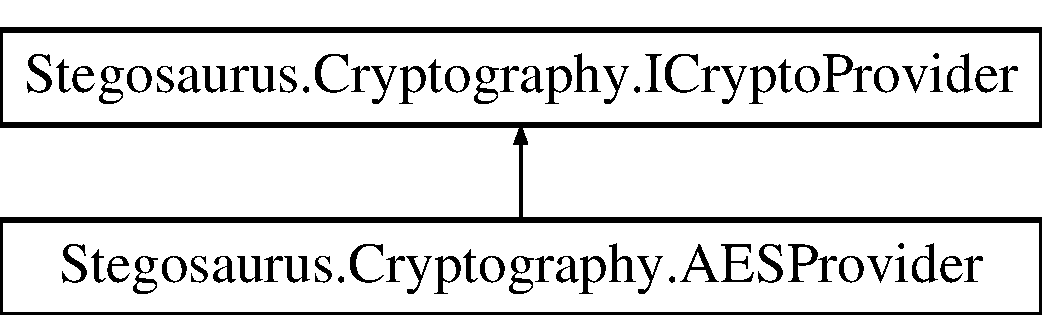
\includegraphics[height=2.000000cm]{class_stegosaurus_1_1_cryptography_1_1_a_e_s_provider}
\end{center}
\end{figure}
\subsection*{Public Member Functions}
\begin{DoxyCompactItemize}
\item 
byte\mbox{[}$\,$\mbox{]} \hyperlink{class_stegosaurus_1_1_cryptography_1_1_a_e_s_provider_a81deb5da864b25f93810afbd8fc6449d}{Encrypt} (byte\mbox{[}$\,$\mbox{]} \+\_\+data)
\begin{DoxyCompactList}\small\item\em Encrypts and returns encrypted data. \end{DoxyCompactList}\item 
byte\mbox{[}$\,$\mbox{]} \hyperlink{class_stegosaurus_1_1_cryptography_1_1_a_e_s_provider_a7f9c88ceae0fb598224b04953ee70e0a}{Decrypt} (byte\mbox{[}$\,$\mbox{]} \+\_\+data)
\begin{DoxyCompactList}\small\item\em Decrypts and returns decrypted data. \end{DoxyCompactList}\item 
byte\mbox{[}$\,$\mbox{]} \hyperlink{class_stegosaurus_1_1_cryptography_1_1_a_e_s_provider_a0e14ad61f9e6bb0555f159e2008153ee}{Generate\+Key} ()
\begin{DoxyCompactList}\small\item\em Generates and returns a key which can be used with the algorithm. \end{DoxyCompactList}\item 
void \hyperlink{class_stegosaurus_1_1_cryptography_1_1_a_e_s_provider_ab9119737779ce4aea6c8c7e6c4725923}{Set\+Key} (string \+\_\+key\+String)
\begin{DoxyCompactList}\small\item\em Set the Key from a string. \end{DoxyCompactList}\end{DoxyCompactItemize}
\subsection*{Public Attributes}
\begin{DoxyCompactItemize}
\item 
string {\bfseries Name} =$>$ \char`\"{}A\+ES\char`\"{}\hypertarget{class_stegosaurus_1_1_cryptography_1_1_a_e_s_provider_aa0a1b3560b0c4a8c2fe39b363e80d853}{}\label{class_stegosaurus_1_1_cryptography_1_1_a_e_s_provider_aa0a1b3560b0c4a8c2fe39b363e80d853}

\item 
int {\bfseries Seed} =$>$ Key == null ? 0 \+: Key.\+Compute\+Hash()\hypertarget{class_stegosaurus_1_1_cryptography_1_1_a_e_s_provider_a2dff11140dc512ee712c08061d878d53}{}\label{class_stegosaurus_1_1_cryptography_1_1_a_e_s_provider_a2dff11140dc512ee712c08061d878d53}

\item 
int {\bfseries Key\+Size} =$>$ 256\hypertarget{class_stegosaurus_1_1_cryptography_1_1_a_e_s_provider_a7383e60bd76754dd3a2e75cb2e06876f}{}\label{class_stegosaurus_1_1_cryptography_1_1_a_e_s_provider_a7383e60bd76754dd3a2e75cb2e06876f}

\end{DoxyCompactItemize}
\subsection*{Properties}
\begin{DoxyCompactItemize}
\item 
byte\mbox{[}$\,$\mbox{]} {\bfseries Key}\hspace{0.3cm}{\ttfamily  \mbox{[}get, set\mbox{]}}\hypertarget{class_stegosaurus_1_1_cryptography_1_1_a_e_s_provider_ad657916d9256db7404625166c03c0603}{}\label{class_stegosaurus_1_1_cryptography_1_1_a_e_s_provider_ad657916d9256db7404625166c03c0603}

\end{DoxyCompactItemize}


\subsection{Member Function Documentation}
\index{Stegosaurus\+::\+Cryptography\+::\+A\+E\+S\+Provider@{Stegosaurus\+::\+Cryptography\+::\+A\+E\+S\+Provider}!Decrypt@{Decrypt}}
\index{Decrypt@{Decrypt}!Stegosaurus\+::\+Cryptography\+::\+A\+E\+S\+Provider@{Stegosaurus\+::\+Cryptography\+::\+A\+E\+S\+Provider}}
\subsubsection[{\texorpdfstring{Decrypt(byte[] \+\_\+data)}{Decrypt(byte[] _data)}}]{\setlength{\rightskip}{0pt plus 5cm}byte \mbox{[}$\,$\mbox{]} Stegosaurus.\+Cryptography.\+A\+E\+S\+Provider.\+Decrypt (
\begin{DoxyParamCaption}
\item[{byte\mbox{[}$\,$\mbox{]}}]{\+\_\+data}
\end{DoxyParamCaption}
)}\hypertarget{class_stegosaurus_1_1_cryptography_1_1_a_e_s_provider_a7f9c88ceae0fb598224b04953ee70e0a}{}\label{class_stegosaurus_1_1_cryptography_1_1_a_e_s_provider_a7f9c88ceae0fb598224b04953ee70e0a}


Decrypts and returns decrypted data. 



Implements \hyperlink{interface_stegosaurus_1_1_cryptography_1_1_i_crypto_provider_a673607b0f3392591db9c647d2499f38d}{Stegosaurus.\+Cryptography.\+I\+Crypto\+Provider}.

\index{Stegosaurus\+::\+Cryptography\+::\+A\+E\+S\+Provider@{Stegosaurus\+::\+Cryptography\+::\+A\+E\+S\+Provider}!Encrypt@{Encrypt}}
\index{Encrypt@{Encrypt}!Stegosaurus\+::\+Cryptography\+::\+A\+E\+S\+Provider@{Stegosaurus\+::\+Cryptography\+::\+A\+E\+S\+Provider}}
\subsubsection[{\texorpdfstring{Encrypt(byte[] \+\_\+data)}{Encrypt(byte[] _data)}}]{\setlength{\rightskip}{0pt plus 5cm}byte \mbox{[}$\,$\mbox{]} Stegosaurus.\+Cryptography.\+A\+E\+S\+Provider.\+Encrypt (
\begin{DoxyParamCaption}
\item[{byte\mbox{[}$\,$\mbox{]}}]{\+\_\+data}
\end{DoxyParamCaption}
)}\hypertarget{class_stegosaurus_1_1_cryptography_1_1_a_e_s_provider_a81deb5da864b25f93810afbd8fc6449d}{}\label{class_stegosaurus_1_1_cryptography_1_1_a_e_s_provider_a81deb5da864b25f93810afbd8fc6449d}


Encrypts and returns encrypted data. 



Implements \hyperlink{interface_stegosaurus_1_1_cryptography_1_1_i_crypto_provider_a2222231bf16ba92e8efc8d515943aacd}{Stegosaurus.\+Cryptography.\+I\+Crypto\+Provider}.

\index{Stegosaurus\+::\+Cryptography\+::\+A\+E\+S\+Provider@{Stegosaurus\+::\+Cryptography\+::\+A\+E\+S\+Provider}!Generate\+Key@{Generate\+Key}}
\index{Generate\+Key@{Generate\+Key}!Stegosaurus\+::\+Cryptography\+::\+A\+E\+S\+Provider@{Stegosaurus\+::\+Cryptography\+::\+A\+E\+S\+Provider}}
\subsubsection[{\texorpdfstring{Generate\+Key()}{GenerateKey()}}]{\setlength{\rightskip}{0pt plus 5cm}byte \mbox{[}$\,$\mbox{]} Stegosaurus.\+Cryptography.\+A\+E\+S\+Provider.\+Generate\+Key (
\begin{DoxyParamCaption}
{}
\end{DoxyParamCaption}
)}\hypertarget{class_stegosaurus_1_1_cryptography_1_1_a_e_s_provider_a0e14ad61f9e6bb0555f159e2008153ee}{}\label{class_stegosaurus_1_1_cryptography_1_1_a_e_s_provider_a0e14ad61f9e6bb0555f159e2008153ee}


Generates and returns a key which can be used with the algorithm. 



Implements \hyperlink{interface_stegosaurus_1_1_cryptography_1_1_i_crypto_provider_ae25c64411409f0cc41c2282030c6dc5c}{Stegosaurus.\+Cryptography.\+I\+Crypto\+Provider}.

\index{Stegosaurus\+::\+Cryptography\+::\+A\+E\+S\+Provider@{Stegosaurus\+::\+Cryptography\+::\+A\+E\+S\+Provider}!Set\+Key@{Set\+Key}}
\index{Set\+Key@{Set\+Key}!Stegosaurus\+::\+Cryptography\+::\+A\+E\+S\+Provider@{Stegosaurus\+::\+Cryptography\+::\+A\+E\+S\+Provider}}
\subsubsection[{\texorpdfstring{Set\+Key(string \+\_\+key\+String)}{SetKey(string _keyString)}}]{\setlength{\rightskip}{0pt plus 5cm}void Stegosaurus.\+Cryptography.\+A\+E\+S\+Provider.\+Set\+Key (
\begin{DoxyParamCaption}
\item[{string}]{\+\_\+key\+String}
\end{DoxyParamCaption}
)}\hypertarget{class_stegosaurus_1_1_cryptography_1_1_a_e_s_provider_ab9119737779ce4aea6c8c7e6c4725923}{}\label{class_stegosaurus_1_1_cryptography_1_1_a_e_s_provider_ab9119737779ce4aea6c8c7e6c4725923}


Set the Key from a string. 



Implements \hyperlink{interface_stegosaurus_1_1_cryptography_1_1_i_crypto_provider_a95c1bb37e8bfdb62e6f66e8094d9d51b}{Stegosaurus.\+Cryptography.\+I\+Crypto\+Provider}.



The documentation for this class was generated from the following file\+:\begin{DoxyCompactItemize}
\item 
Steganography/\+Stegosaurus/\+Cryptography/A\+E\+S\+Provider.\+cs\end{DoxyCompactItemize}

\hypertarget{class_stegosaurus_1_1_carrier_1_1_audio_carrier}{}\section{Stegosaurus.\+Carrier.\+Audio\+Carrier Class Reference}
\label{class_stegosaurus_1_1_carrier_1_1_audio_carrier}\index{Stegosaurus.\+Carrier.\+Audio\+Carrier@{Stegosaurus.\+Carrier.\+Audio\+Carrier}}
Inheritance diagram for Stegosaurus.\+Carrier.\+Audio\+Carrier\+:\begin{figure}[H]
\begin{center}
\leavevmode
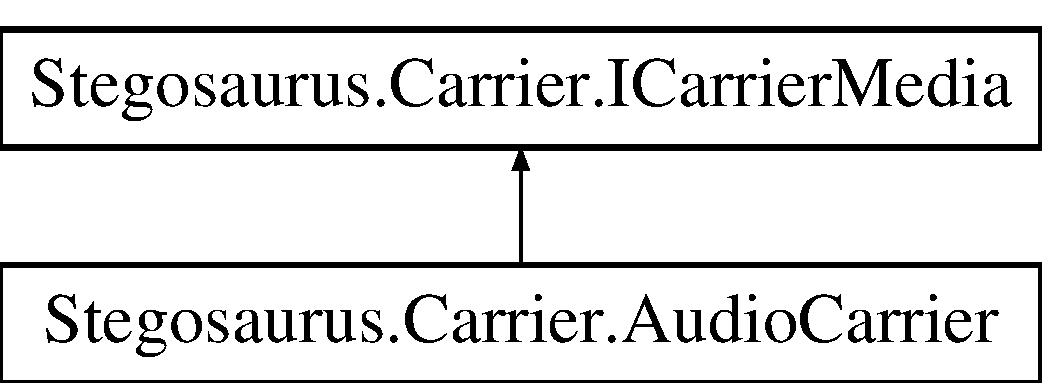
\includegraphics[height=2.000000cm]{class_stegosaurus_1_1_carrier_1_1_audio_carrier}
\end{center}
\end{figure}
\subsection*{Public Member Functions}
\begin{DoxyCompactItemize}
\item 
\hyperlink{class_stegosaurus_1_1_carrier_1_1_audio_carrier_abf7e6bb9093fdb385f11d19f1ef188dd}{Audio\+Carrier} (string \+\_\+file\+Path)
\begin{DoxyCompactList}\small\item\em Construct an \hyperlink{class_stegosaurus_1_1_carrier_1_1_audio_carrier}{Audio\+Carrier} from a file path. \end{DoxyCompactList}\item 
void \hyperlink{class_stegosaurus_1_1_carrier_1_1_audio_carrier_a2d02a6c7c6ceda7a0a956ca2ab92a03d}{Decode} ()
\begin{DoxyCompactList}\small\item\em Decodes the carrier media and sets Byte\+Array to the inner data. \end{DoxyCompactList}\item 
void \hyperlink{class_stegosaurus_1_1_carrier_1_1_audio_carrier_aacb57072610e4c5d59496d7e9c2262f0}{Encode} ()
\begin{DoxyCompactList}\small\item\em Encodes Byte\+Array back into the carrier media. \end{DoxyCompactList}\item 
void \hyperlink{class_stegosaurus_1_1_carrier_1_1_audio_carrier_ac703d4709853222c6dcc98d12f6c9130}{Save\+To\+File} (string \+\_\+destination)
\begin{DoxyCompactList}\small\item\em Saves the carrier media to the specified destination. \end{DoxyCompactList}\end{DoxyCompactItemize}
\subsection*{Public Attributes}
\begin{DoxyCompactItemize}
\item 
int {\bfseries Bytes\+Per\+Sample} =$>$ audio\+File.\+Bits\+Per\+Sample / 8\hypertarget{class_stegosaurus_1_1_carrier_1_1_audio_carrier_a7db55f75539ae6856d97e4cd7bb57bcd}{}\label{class_stegosaurus_1_1_carrier_1_1_audio_carrier_a7db55f75539ae6856d97e4cd7bb57bcd}

\end{DoxyCompactItemize}
\subsection*{Properties}
\begin{DoxyCompactItemize}
\item 
byte\mbox{[}$\,$\mbox{]} {\bfseries Byte\+Array}\hspace{0.3cm}{\ttfamily  \mbox{[}get, set\mbox{]}}\hypertarget{class_stegosaurus_1_1_carrier_1_1_audio_carrier_a54cd42103b6233e81a61650be8634281}{}\label{class_stegosaurus_1_1_carrier_1_1_audio_carrier_a54cd42103b6233e81a61650be8634281}

\end{DoxyCompactItemize}


\subsection{Constructor \& Destructor Documentation}
\index{Stegosaurus\+::\+Carrier\+::\+Audio\+Carrier@{Stegosaurus\+::\+Carrier\+::\+Audio\+Carrier}!Audio\+Carrier@{Audio\+Carrier}}
\index{Audio\+Carrier@{Audio\+Carrier}!Stegosaurus\+::\+Carrier\+::\+Audio\+Carrier@{Stegosaurus\+::\+Carrier\+::\+Audio\+Carrier}}
\subsubsection[{\texorpdfstring{Audio\+Carrier(string \+\_\+file\+Path)}{AudioCarrier(string _filePath)}}]{\setlength{\rightskip}{0pt plus 5cm}Stegosaurus.\+Carrier.\+Audio\+Carrier.\+Audio\+Carrier (
\begin{DoxyParamCaption}
\item[{string}]{\+\_\+file\+Path}
\end{DoxyParamCaption}
)}\hypertarget{class_stegosaurus_1_1_carrier_1_1_audio_carrier_abf7e6bb9093fdb385f11d19f1ef188dd}{}\label{class_stegosaurus_1_1_carrier_1_1_audio_carrier_abf7e6bb9093fdb385f11d19f1ef188dd}


Construct an \hyperlink{class_stegosaurus_1_1_carrier_1_1_audio_carrier}{Audio\+Carrier} from a file path. 



\subsection{Member Function Documentation}
\index{Stegosaurus\+::\+Carrier\+::\+Audio\+Carrier@{Stegosaurus\+::\+Carrier\+::\+Audio\+Carrier}!Decode@{Decode}}
\index{Decode@{Decode}!Stegosaurus\+::\+Carrier\+::\+Audio\+Carrier@{Stegosaurus\+::\+Carrier\+::\+Audio\+Carrier}}
\subsubsection[{\texorpdfstring{Decode()}{Decode()}}]{\setlength{\rightskip}{0pt plus 5cm}void Stegosaurus.\+Carrier.\+Audio\+Carrier.\+Decode (
\begin{DoxyParamCaption}
{}
\end{DoxyParamCaption}
)}\hypertarget{class_stegosaurus_1_1_carrier_1_1_audio_carrier_a2d02a6c7c6ceda7a0a956ca2ab92a03d}{}\label{class_stegosaurus_1_1_carrier_1_1_audio_carrier_a2d02a6c7c6ceda7a0a956ca2ab92a03d}


Decodes the carrier media and sets Byte\+Array to the inner data. 



Implements \hyperlink{interface_stegosaurus_1_1_carrier_1_1_i_carrier_media_a863ecfa01ac50d9bb4a7619ce3f14fad}{Stegosaurus.\+Carrier.\+I\+Carrier\+Media}.

\index{Stegosaurus\+::\+Carrier\+::\+Audio\+Carrier@{Stegosaurus\+::\+Carrier\+::\+Audio\+Carrier}!Encode@{Encode}}
\index{Encode@{Encode}!Stegosaurus\+::\+Carrier\+::\+Audio\+Carrier@{Stegosaurus\+::\+Carrier\+::\+Audio\+Carrier}}
\subsubsection[{\texorpdfstring{Encode()}{Encode()}}]{\setlength{\rightskip}{0pt plus 5cm}void Stegosaurus.\+Carrier.\+Audio\+Carrier.\+Encode (
\begin{DoxyParamCaption}
{}
\end{DoxyParamCaption}
)}\hypertarget{class_stegosaurus_1_1_carrier_1_1_audio_carrier_aacb57072610e4c5d59496d7e9c2262f0}{}\label{class_stegosaurus_1_1_carrier_1_1_audio_carrier_aacb57072610e4c5d59496d7e9c2262f0}


Encodes Byte\+Array back into the carrier media. 



Implements \hyperlink{interface_stegosaurus_1_1_carrier_1_1_i_carrier_media_ac7d498eec146a74dbbaa2bd60e5bdce7}{Stegosaurus.\+Carrier.\+I\+Carrier\+Media}.

\index{Stegosaurus\+::\+Carrier\+::\+Audio\+Carrier@{Stegosaurus\+::\+Carrier\+::\+Audio\+Carrier}!Save\+To\+File@{Save\+To\+File}}
\index{Save\+To\+File@{Save\+To\+File}!Stegosaurus\+::\+Carrier\+::\+Audio\+Carrier@{Stegosaurus\+::\+Carrier\+::\+Audio\+Carrier}}
\subsubsection[{\texorpdfstring{Save\+To\+File(string \+\_\+destination)}{SaveToFile(string _destination)}}]{\setlength{\rightskip}{0pt plus 5cm}void Stegosaurus.\+Carrier.\+Audio\+Carrier.\+Save\+To\+File (
\begin{DoxyParamCaption}
\item[{string}]{\+\_\+destination}
\end{DoxyParamCaption}
)}\hypertarget{class_stegosaurus_1_1_carrier_1_1_audio_carrier_ac703d4709853222c6dcc98d12f6c9130}{}\label{class_stegosaurus_1_1_carrier_1_1_audio_carrier_ac703d4709853222c6dcc98d12f6c9130}


Saves the carrier media to the specified destination. 



Implements \hyperlink{interface_stegosaurus_1_1_carrier_1_1_i_carrier_media_a419a6ed82dc1053f25e42a26e2fbade3}{Stegosaurus.\+Carrier.\+I\+Carrier\+Media}.



The documentation for this class was generated from the following file\+:\begin{DoxyCompactItemize}
\item 
Steganography/\+Stegosaurus/\+Carrier/Audio\+Carrier.\+cs\end{DoxyCompactItemize}

\hypertarget{class_stegosaurus_1_1_carrier_1_1_audio_formats_1_1_audio_file}{}\section{Stegosaurus.\+Carrier.\+Audio\+Formats.\+Audio\+File Class Reference}
\label{class_stegosaurus_1_1_carrier_1_1_audio_formats_1_1_audio_file}\index{Stegosaurus.\+Carrier.\+Audio\+Formats.\+Audio\+File@{Stegosaurus.\+Carrier.\+Audio\+Formats.\+Audio\+File}}
Inheritance diagram for Stegosaurus.\+Carrier.\+Audio\+Formats.\+Audio\+File\+:\begin{figure}[H]
\begin{center}
\leavevmode
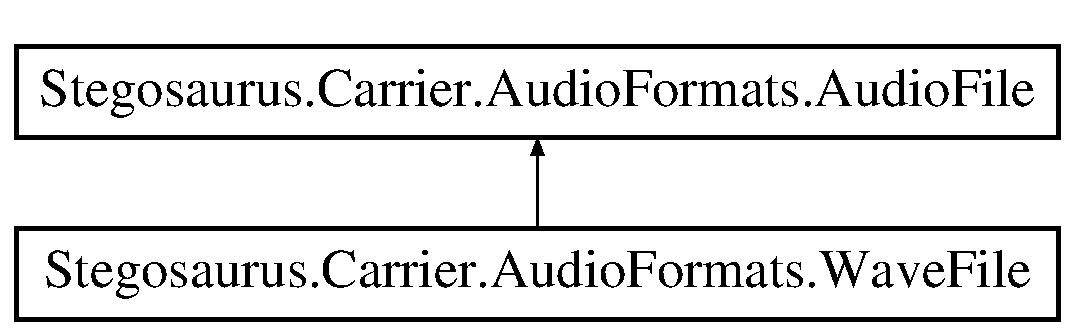
\includegraphics[height=2.000000cm]{class_stegosaurus_1_1_carrier_1_1_audio_formats_1_1_audio_file}
\end{center}
\end{figure}
\subsection*{Public Member Functions}
\begin{DoxyCompactItemize}
\item 
abstract void \hyperlink{class_stegosaurus_1_1_carrier_1_1_audio_formats_1_1_audio_file_a52a9349e3c5cf18eca6f61cee8d81d2b}{Parse} (string \+\_\+file\+Path)
\begin{DoxyCompactList}\small\item\em Parses an audio file by reading its headers and samples. \end{DoxyCompactList}\item 
abstract byte\mbox{[}$\,$\mbox{]} \hyperlink{class_stegosaurus_1_1_carrier_1_1_audio_formats_1_1_audio_file_ac62f509a70ce93baab9b8112198ff6ac}{To\+Array} ()
\begin{DoxyCompactList}\small\item\em Reconstructs and returns the entire byte array of the file, including headers. \end{DoxyCompactList}\item 
virtual void \hyperlink{class_stegosaurus_1_1_carrier_1_1_audio_formats_1_1_audio_file_a2a630f7f7001762580a9c8284d90dd5f}{Set\+Inner\+Data} (byte\mbox{[}$\,$\mbox{]} \+\_\+inner\+Data)
\begin{DoxyCompactList}\small\item\em Sets the inner\+Data of the audio file, which contains the original samples. \end{DoxyCompactList}\item 
virtual byte\mbox{[}$\,$\mbox{]} \hyperlink{class_stegosaurus_1_1_carrier_1_1_audio_formats_1_1_audio_file_aab99c651bb658ffa232aa21bab968124}{Copy\+Inner\+Data} ()
\begin{DoxyCompactList}\small\item\em Returns a clone of the inner\+Data array which can be manipulated by an algorithm. \end{DoxyCompactList}\end{DoxyCompactItemize}
\subsection*{Protected Member Functions}
\begin{DoxyCompactItemize}
\item 
\hyperlink{class_stegosaurus_1_1_carrier_1_1_audio_formats_1_1_audio_file_ad64ea28a0bf30b61f69174c094a9539c}{Audio\+File} (string \+\_\+file\+Path)
\begin{DoxyCompactList}\small\item\em Construct an \hyperlink{class_stegosaurus_1_1_carrier_1_1_audio_formats_1_1_audio_file}{Audio\+File} from a file path. \end{DoxyCompactList}\end{DoxyCompactItemize}
\subsection*{Protected Attributes}
\begin{DoxyCompactItemize}
\item 
byte\mbox{[}$\,$\mbox{]} {\bfseries inner\+Data}\hypertarget{class_stegosaurus_1_1_carrier_1_1_audio_formats_1_1_audio_file_ab2ed9d7628f413b6930d4e16bfe54c1e}{}\label{class_stegosaurus_1_1_carrier_1_1_audio_formats_1_1_audio_file_ab2ed9d7628f413b6930d4e16bfe54c1e}

\end{DoxyCompactItemize}
\subsection*{Properties}
\begin{DoxyCompactItemize}
\item 
short \hyperlink{class_stegosaurus_1_1_carrier_1_1_audio_formats_1_1_audio_file_a038e85d44a449672c16e27c111326af7}{Number\+Of\+Channels}\hspace{0.3cm}{\ttfamily  \mbox{[}get, protected set\mbox{]}}
\begin{DoxyCompactList}\small\item\em Get or set the number of channels. \end{DoxyCompactList}\item 
int \hyperlink{class_stegosaurus_1_1_carrier_1_1_audio_formats_1_1_audio_file_a4d08e828f8189faeb1de0a639a07ac5e}{Sample\+Rate}\hspace{0.3cm}{\ttfamily  \mbox{[}get, protected set\mbox{]}}
\begin{DoxyCompactList}\small\item\em Get or set the sample rate. \end{DoxyCompactList}\item 
int \hyperlink{class_stegosaurus_1_1_carrier_1_1_audio_formats_1_1_audio_file_a4cc1b36f47de282eab3b2798327d70e4}{Byte\+Rate}\hspace{0.3cm}{\ttfamily  \mbox{[}get, protected set\mbox{]}}
\begin{DoxyCompactList}\small\item\em Get or set the byte rate. \end{DoxyCompactList}\item 
short \hyperlink{class_stegosaurus_1_1_carrier_1_1_audio_formats_1_1_audio_file_a99d78d8cf74a9bfccfc5aae75accb7b6}{Block\+Align}\hspace{0.3cm}{\ttfamily  \mbox{[}get, protected set\mbox{]}}
\begin{DoxyCompactList}\small\item\em Get or set the block align. \end{DoxyCompactList}\item 
short \hyperlink{class_stegosaurus_1_1_carrier_1_1_audio_formats_1_1_audio_file_a29d9405c31acf979205938e419b3c337}{Bits\+Per\+Sample}\hspace{0.3cm}{\ttfamily  \mbox{[}get, protected set\mbox{]}}
\begin{DoxyCompactList}\small\item\em Get or set the bits per sample. \end{DoxyCompactList}\end{DoxyCompactItemize}


\subsection{Constructor \& Destructor Documentation}
\index{Stegosaurus\+::\+Carrier\+::\+Audio\+Formats\+::\+Audio\+File@{Stegosaurus\+::\+Carrier\+::\+Audio\+Formats\+::\+Audio\+File}!Audio\+File@{Audio\+File}}
\index{Audio\+File@{Audio\+File}!Stegosaurus\+::\+Carrier\+::\+Audio\+Formats\+::\+Audio\+File@{Stegosaurus\+::\+Carrier\+::\+Audio\+Formats\+::\+Audio\+File}}
\subsubsection[{\texorpdfstring{Audio\+File(string \+\_\+file\+Path)}{AudioFile(string _filePath)}}]{\setlength{\rightskip}{0pt plus 5cm}Stegosaurus.\+Carrier.\+Audio\+Formats.\+Audio\+File.\+Audio\+File (
\begin{DoxyParamCaption}
\item[{string}]{\+\_\+file\+Path}
\end{DoxyParamCaption}
)\hspace{0.3cm}{\ttfamily [protected]}}\hypertarget{class_stegosaurus_1_1_carrier_1_1_audio_formats_1_1_audio_file_ad64ea28a0bf30b61f69174c094a9539c}{}\label{class_stegosaurus_1_1_carrier_1_1_audio_formats_1_1_audio_file_ad64ea28a0bf30b61f69174c094a9539c}


Construct an \hyperlink{class_stegosaurus_1_1_carrier_1_1_audio_formats_1_1_audio_file}{Audio\+File} from a file path. 



\subsection{Member Function Documentation}
\index{Stegosaurus\+::\+Carrier\+::\+Audio\+Formats\+::\+Audio\+File@{Stegosaurus\+::\+Carrier\+::\+Audio\+Formats\+::\+Audio\+File}!Copy\+Inner\+Data@{Copy\+Inner\+Data}}
\index{Copy\+Inner\+Data@{Copy\+Inner\+Data}!Stegosaurus\+::\+Carrier\+::\+Audio\+Formats\+::\+Audio\+File@{Stegosaurus\+::\+Carrier\+::\+Audio\+Formats\+::\+Audio\+File}}
\subsubsection[{\texorpdfstring{Copy\+Inner\+Data()}{CopyInnerData()}}]{\setlength{\rightskip}{0pt plus 5cm}virtual byte \mbox{[}$\,$\mbox{]} Stegosaurus.\+Carrier.\+Audio\+Formats.\+Audio\+File.\+Copy\+Inner\+Data (
\begin{DoxyParamCaption}
{}
\end{DoxyParamCaption}
)\hspace{0.3cm}{\ttfamily [virtual]}}\hypertarget{class_stegosaurus_1_1_carrier_1_1_audio_formats_1_1_audio_file_aab99c651bb658ffa232aa21bab968124}{}\label{class_stegosaurus_1_1_carrier_1_1_audio_formats_1_1_audio_file_aab99c651bb658ffa232aa21bab968124}


Returns a clone of the inner\+Data array which can be manipulated by an algorithm. 

\index{Stegosaurus\+::\+Carrier\+::\+Audio\+Formats\+::\+Audio\+File@{Stegosaurus\+::\+Carrier\+::\+Audio\+Formats\+::\+Audio\+File}!Parse@{Parse}}
\index{Parse@{Parse}!Stegosaurus\+::\+Carrier\+::\+Audio\+Formats\+::\+Audio\+File@{Stegosaurus\+::\+Carrier\+::\+Audio\+Formats\+::\+Audio\+File}}
\subsubsection[{\texorpdfstring{Parse(string \+\_\+file\+Path)}{Parse(string _filePath)}}]{\setlength{\rightskip}{0pt plus 5cm}abstract void Stegosaurus.\+Carrier.\+Audio\+Formats.\+Audio\+File.\+Parse (
\begin{DoxyParamCaption}
\item[{string}]{\+\_\+file\+Path}
\end{DoxyParamCaption}
)\hspace{0.3cm}{\ttfamily [pure virtual]}}\hypertarget{class_stegosaurus_1_1_carrier_1_1_audio_formats_1_1_audio_file_a52a9349e3c5cf18eca6f61cee8d81d2b}{}\label{class_stegosaurus_1_1_carrier_1_1_audio_formats_1_1_audio_file_a52a9349e3c5cf18eca6f61cee8d81d2b}


Parses an audio file by reading its headers and samples. 



Implemented in \hyperlink{class_stegosaurus_1_1_carrier_1_1_audio_formats_1_1_wave_file_aa18e174d66b4d3fefef8683b35946120}{Stegosaurus.\+Carrier.\+Audio\+Formats.\+Wave\+File}.

\index{Stegosaurus\+::\+Carrier\+::\+Audio\+Formats\+::\+Audio\+File@{Stegosaurus\+::\+Carrier\+::\+Audio\+Formats\+::\+Audio\+File}!Set\+Inner\+Data@{Set\+Inner\+Data}}
\index{Set\+Inner\+Data@{Set\+Inner\+Data}!Stegosaurus\+::\+Carrier\+::\+Audio\+Formats\+::\+Audio\+File@{Stegosaurus\+::\+Carrier\+::\+Audio\+Formats\+::\+Audio\+File}}
\subsubsection[{\texorpdfstring{Set\+Inner\+Data(byte[] \+\_\+inner\+Data)}{SetInnerData(byte[] _innerData)}}]{\setlength{\rightskip}{0pt plus 5cm}virtual void Stegosaurus.\+Carrier.\+Audio\+Formats.\+Audio\+File.\+Set\+Inner\+Data (
\begin{DoxyParamCaption}
\item[{byte\mbox{[}$\,$\mbox{]}}]{\+\_\+inner\+Data}
\end{DoxyParamCaption}
)\hspace{0.3cm}{\ttfamily [virtual]}}\hypertarget{class_stegosaurus_1_1_carrier_1_1_audio_formats_1_1_audio_file_a2a630f7f7001762580a9c8284d90dd5f}{}\label{class_stegosaurus_1_1_carrier_1_1_audio_formats_1_1_audio_file_a2a630f7f7001762580a9c8284d90dd5f}


Sets the inner\+Data of the audio file, which contains the original samples. 

\index{Stegosaurus\+::\+Carrier\+::\+Audio\+Formats\+::\+Audio\+File@{Stegosaurus\+::\+Carrier\+::\+Audio\+Formats\+::\+Audio\+File}!To\+Array@{To\+Array}}
\index{To\+Array@{To\+Array}!Stegosaurus\+::\+Carrier\+::\+Audio\+Formats\+::\+Audio\+File@{Stegosaurus\+::\+Carrier\+::\+Audio\+Formats\+::\+Audio\+File}}
\subsubsection[{\texorpdfstring{To\+Array()}{ToArray()}}]{\setlength{\rightskip}{0pt plus 5cm}abstract byte \mbox{[}$\,$\mbox{]} Stegosaurus.\+Carrier.\+Audio\+Formats.\+Audio\+File.\+To\+Array (
\begin{DoxyParamCaption}
{}
\end{DoxyParamCaption}
)\hspace{0.3cm}{\ttfamily [pure virtual]}}\hypertarget{class_stegosaurus_1_1_carrier_1_1_audio_formats_1_1_audio_file_ac62f509a70ce93baab9b8112198ff6ac}{}\label{class_stegosaurus_1_1_carrier_1_1_audio_formats_1_1_audio_file_ac62f509a70ce93baab9b8112198ff6ac}


Reconstructs and returns the entire byte array of the file, including headers. 



Implemented in \hyperlink{class_stegosaurus_1_1_carrier_1_1_audio_formats_1_1_wave_file_a3de2c6ede07d46d1bfc3082fcf07d015}{Stegosaurus.\+Carrier.\+Audio\+Formats.\+Wave\+File}.



\subsection{Property Documentation}
\index{Stegosaurus\+::\+Carrier\+::\+Audio\+Formats\+::\+Audio\+File@{Stegosaurus\+::\+Carrier\+::\+Audio\+Formats\+::\+Audio\+File}!Bits\+Per\+Sample@{Bits\+Per\+Sample}}
\index{Bits\+Per\+Sample@{Bits\+Per\+Sample}!Stegosaurus\+::\+Carrier\+::\+Audio\+Formats\+::\+Audio\+File@{Stegosaurus\+::\+Carrier\+::\+Audio\+Formats\+::\+Audio\+File}}
\subsubsection[{\texorpdfstring{Bits\+Per\+Sample}{BitsPerSample}}]{\setlength{\rightskip}{0pt plus 5cm}short Stegosaurus.\+Carrier.\+Audio\+Formats.\+Audio\+File.\+Bits\+Per\+Sample\hspace{0.3cm}{\ttfamily [get]}, {\ttfamily [protected set]}}\hypertarget{class_stegosaurus_1_1_carrier_1_1_audio_formats_1_1_audio_file_a29d9405c31acf979205938e419b3c337}{}\label{class_stegosaurus_1_1_carrier_1_1_audio_formats_1_1_audio_file_a29d9405c31acf979205938e419b3c337}


Get or set the bits per sample. 

\index{Stegosaurus\+::\+Carrier\+::\+Audio\+Formats\+::\+Audio\+File@{Stegosaurus\+::\+Carrier\+::\+Audio\+Formats\+::\+Audio\+File}!Block\+Align@{Block\+Align}}
\index{Block\+Align@{Block\+Align}!Stegosaurus\+::\+Carrier\+::\+Audio\+Formats\+::\+Audio\+File@{Stegosaurus\+::\+Carrier\+::\+Audio\+Formats\+::\+Audio\+File}}
\subsubsection[{\texorpdfstring{Block\+Align}{BlockAlign}}]{\setlength{\rightskip}{0pt plus 5cm}short Stegosaurus.\+Carrier.\+Audio\+Formats.\+Audio\+File.\+Block\+Align\hspace{0.3cm}{\ttfamily [get]}, {\ttfamily [protected set]}}\hypertarget{class_stegosaurus_1_1_carrier_1_1_audio_formats_1_1_audio_file_a99d78d8cf74a9bfccfc5aae75accb7b6}{}\label{class_stegosaurus_1_1_carrier_1_1_audio_formats_1_1_audio_file_a99d78d8cf74a9bfccfc5aae75accb7b6}


Get or set the block align. 

\index{Stegosaurus\+::\+Carrier\+::\+Audio\+Formats\+::\+Audio\+File@{Stegosaurus\+::\+Carrier\+::\+Audio\+Formats\+::\+Audio\+File}!Byte\+Rate@{Byte\+Rate}}
\index{Byte\+Rate@{Byte\+Rate}!Stegosaurus\+::\+Carrier\+::\+Audio\+Formats\+::\+Audio\+File@{Stegosaurus\+::\+Carrier\+::\+Audio\+Formats\+::\+Audio\+File}}
\subsubsection[{\texorpdfstring{Byte\+Rate}{ByteRate}}]{\setlength{\rightskip}{0pt plus 5cm}int Stegosaurus.\+Carrier.\+Audio\+Formats.\+Audio\+File.\+Byte\+Rate\hspace{0.3cm}{\ttfamily [get]}, {\ttfamily [protected set]}}\hypertarget{class_stegosaurus_1_1_carrier_1_1_audio_formats_1_1_audio_file_a4cc1b36f47de282eab3b2798327d70e4}{}\label{class_stegosaurus_1_1_carrier_1_1_audio_formats_1_1_audio_file_a4cc1b36f47de282eab3b2798327d70e4}


Get or set the byte rate. 

\index{Stegosaurus\+::\+Carrier\+::\+Audio\+Formats\+::\+Audio\+File@{Stegosaurus\+::\+Carrier\+::\+Audio\+Formats\+::\+Audio\+File}!Number\+Of\+Channels@{Number\+Of\+Channels}}
\index{Number\+Of\+Channels@{Number\+Of\+Channels}!Stegosaurus\+::\+Carrier\+::\+Audio\+Formats\+::\+Audio\+File@{Stegosaurus\+::\+Carrier\+::\+Audio\+Formats\+::\+Audio\+File}}
\subsubsection[{\texorpdfstring{Number\+Of\+Channels}{NumberOfChannels}}]{\setlength{\rightskip}{0pt plus 5cm}short Stegosaurus.\+Carrier.\+Audio\+Formats.\+Audio\+File.\+Number\+Of\+Channels\hspace{0.3cm}{\ttfamily [get]}, {\ttfamily [protected set]}}\hypertarget{class_stegosaurus_1_1_carrier_1_1_audio_formats_1_1_audio_file_a038e85d44a449672c16e27c111326af7}{}\label{class_stegosaurus_1_1_carrier_1_1_audio_formats_1_1_audio_file_a038e85d44a449672c16e27c111326af7}


Get or set the number of channels. 

\index{Stegosaurus\+::\+Carrier\+::\+Audio\+Formats\+::\+Audio\+File@{Stegosaurus\+::\+Carrier\+::\+Audio\+Formats\+::\+Audio\+File}!Sample\+Rate@{Sample\+Rate}}
\index{Sample\+Rate@{Sample\+Rate}!Stegosaurus\+::\+Carrier\+::\+Audio\+Formats\+::\+Audio\+File@{Stegosaurus\+::\+Carrier\+::\+Audio\+Formats\+::\+Audio\+File}}
\subsubsection[{\texorpdfstring{Sample\+Rate}{SampleRate}}]{\setlength{\rightskip}{0pt plus 5cm}int Stegosaurus.\+Carrier.\+Audio\+Formats.\+Audio\+File.\+Sample\+Rate\hspace{0.3cm}{\ttfamily [get]}, {\ttfamily [protected set]}}\hypertarget{class_stegosaurus_1_1_carrier_1_1_audio_formats_1_1_audio_file_a4d08e828f8189faeb1de0a639a07ac5e}{}\label{class_stegosaurus_1_1_carrier_1_1_audio_formats_1_1_audio_file_a4d08e828f8189faeb1de0a639a07ac5e}


Get or set the sample rate. 



The documentation for this class was generated from the following file\+:\begin{DoxyCompactItemize}
\item 
Steganography/\+Stegosaurus/\+Carrier/\+Audio\+Formats/Audio\+File.\+cs\end{DoxyCompactItemize}

\hypertarget{class_stegosaurus_1_1_utility_1_1_input_types_1_1_carrier_type}{}\section{Stegosaurus.\+Utility.\+Input\+Types.\+Carrier\+Type Class Reference}
\label{class_stegosaurus_1_1_utility_1_1_input_types_1_1_carrier_type}\index{Stegosaurus.\+Utility.\+Input\+Types.\+Carrier\+Type@{Stegosaurus.\+Utility.\+Input\+Types.\+Carrier\+Type}}
Inheritance diagram for Stegosaurus.\+Utility.\+Input\+Types.\+Carrier\+Type\+:\begin{figure}[H]
\begin{center}
\leavevmode
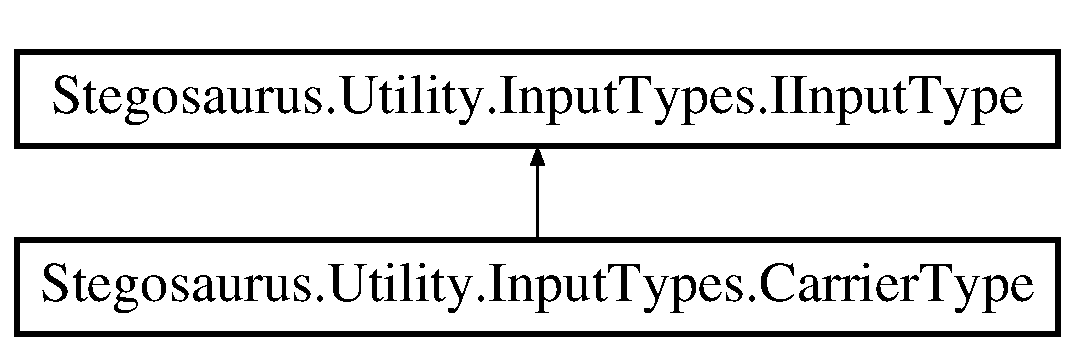
\includegraphics[height=2.000000cm]{class_stegosaurus_1_1_utility_1_1_input_types_1_1_carrier_type}
\end{center}
\end{figure}
\subsection*{Public Member Functions}
\begin{DoxyCompactItemize}
\item 
{\bfseries Carrier\+Type} (string \+\_\+file\+Path)\hypertarget{class_stegosaurus_1_1_utility_1_1_input_types_1_1_carrier_type_a10e94c9805a3fe2f6e076de6eaa966bf}{}\label{class_stegosaurus_1_1_utility_1_1_input_types_1_1_carrier_type_a10e94c9805a3fe2f6e076de6eaa966bf}

\end{DoxyCompactItemize}
\subsection*{Properties}
\begin{DoxyCompactItemize}
\item 
string {\bfseries File\+Path}\hspace{0.3cm}{\ttfamily  \mbox{[}get, set\mbox{]}}\hypertarget{class_stegosaurus_1_1_utility_1_1_input_types_1_1_carrier_type_aecf43bad73d78ed8ee181af8bdf0a323}{}\label{class_stegosaurus_1_1_utility_1_1_input_types_1_1_carrier_type_aecf43bad73d78ed8ee181af8bdf0a323}

\end{DoxyCompactItemize}


The documentation for this class was generated from the following file\+:\begin{DoxyCompactItemize}
\item 
Steganography/\+Stegosaurus/\+Utility/\+Input\+Types/Carrier\+Type.\+cs\end{DoxyCompactItemize}

\hypertarget{class_stegosaurus_1_1_extensions_1_1_input_extensions_1_1_carrier_type}{}\section{Stegosaurus.\+Extensions.\+Input\+Extensions.\+Carrier\+Type Class Reference}
\label{class_stegosaurus_1_1_extensions_1_1_input_extensions_1_1_carrier_type}\index{Stegosaurus.\+Extensions.\+Input\+Extensions.\+Carrier\+Type@{Stegosaurus.\+Extensions.\+Input\+Extensions.\+Carrier\+Type}}
Inheritance diagram for Stegosaurus.\+Extensions.\+Input\+Extensions.\+Carrier\+Type\+:\begin{figure}[H]
\begin{center}
\leavevmode
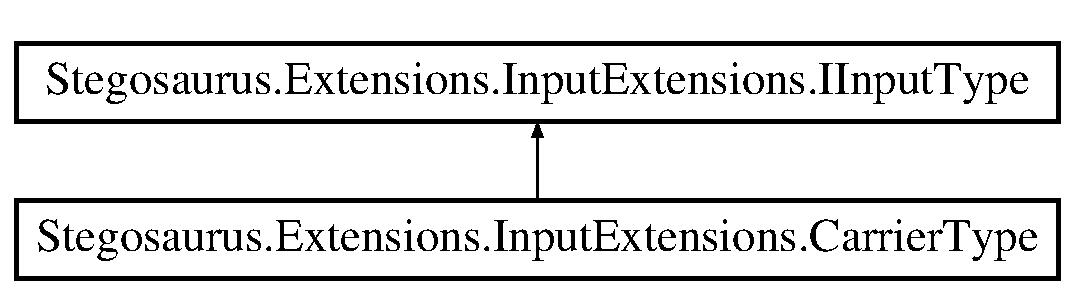
\includegraphics[height=2.000000cm]{class_stegosaurus_1_1_extensions_1_1_input_extensions_1_1_carrier_type}
\end{center}
\end{figure}
\subsection*{Public Member Functions}
\begin{DoxyCompactItemize}
\item 
{\bfseries Carrier\+Type} (string \+\_\+file\+Path)\hypertarget{class_stegosaurus_1_1_extensions_1_1_input_extensions_1_1_carrier_type_ae569efa478f5707bd4bfd0bb865f5fe0}{}\label{class_stegosaurus_1_1_extensions_1_1_input_extensions_1_1_carrier_type_ae569efa478f5707bd4bfd0bb865f5fe0}

\end{DoxyCompactItemize}
\subsection*{Properties}
\begin{DoxyCompactItemize}
\item 
string {\bfseries File\+Path}\hspace{0.3cm}{\ttfamily  \mbox{[}get, set\mbox{]}}\hypertarget{class_stegosaurus_1_1_extensions_1_1_input_extensions_1_1_carrier_type_a6a473cc6d65d9d2360cf644e63f34478}{}\label{class_stegosaurus_1_1_extensions_1_1_input_extensions_1_1_carrier_type_a6a473cc6d65d9d2360cf644e63f34478}

\end{DoxyCompactItemize}


The documentation for this class was generated from the following file\+:\begin{DoxyCompactItemize}
\item 
Steganography/\+Stegosaurus/\+Extensions/\+Input\+Extensions/Carrier\+Type.\+cs\end{DoxyCompactItemize}

\hypertarget{class_stegosaurus_1_1_algorithm_1_1_common_sample_algorithm}{}\section{Stegosaurus.\+Algorithm.\+Common\+Sample\+Algorithm Class Reference}
\label{class_stegosaurus_1_1_algorithm_1_1_common_sample_algorithm}\index{Stegosaurus.\+Algorithm.\+Common\+Sample\+Algorithm@{Stegosaurus.\+Algorithm.\+Common\+Sample\+Algorithm}}
Inheritance diagram for Stegosaurus.\+Algorithm.\+Common\+Sample\+Algorithm\+:\begin{figure}[H]
\begin{center}
\leavevmode
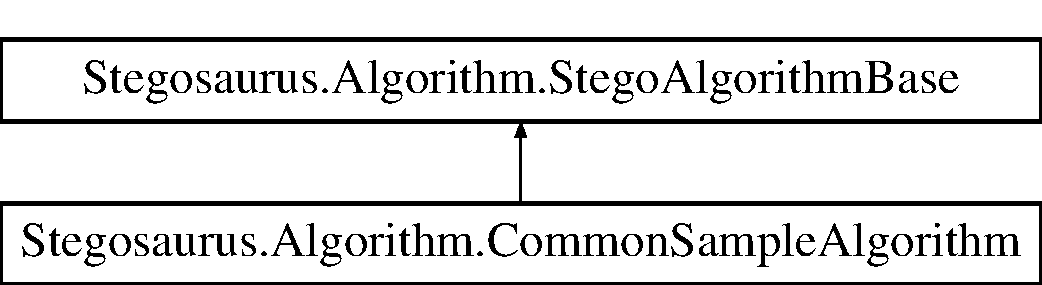
\includegraphics[height=2.000000cm]{class_stegosaurus_1_1_algorithm_1_1_common_sample_algorithm}
\end{center}
\end{figure}
\subsection*{Public Member Functions}
\begin{DoxyCompactItemize}
\item 
override void \hyperlink{class_stegosaurus_1_1_algorithm_1_1_common_sample_algorithm_ab25967eede4bbf5ea54d64b168e4ae73}{Embed} (\hyperlink{class_stegosaurus_1_1_stego_message}{Stego\+Message} message, I\+Progress$<$ int $>$ \+\_\+progress, Cancellation\+Token \+\_\+ct)
\begin{DoxyCompactList}\small\item\em Embeds a \hyperlink{class_stegosaurus_1_1_stego_message}{Stego\+Message} in the public Byte\+Array of the Carrier\+Media. \end{DoxyCompactList}\item 
override \hyperlink{class_stegosaurus_1_1_stego_message}{Stego\+Message} \hyperlink{class_stegosaurus_1_1_algorithm_1_1_common_sample_algorithm_aab6487375c07bb4e77c719bb96605ad4}{Extract} ()
\begin{DoxyCompactList}\small\item\em Returns a \hyperlink{class_stegosaurus_1_1_stego_message}{Stego\+Message} by extracting from the public Byte\+Array of the Carrier\+Media. \end{DoxyCompactList}\item 
override long \hyperlink{class_stegosaurus_1_1_algorithm_1_1_common_sample_algorithm_aeb094a2d87af7b06f7710b79915164d8}{Compute\+Bandwidth} ()
\begin{DoxyCompactList}\small\item\em Returns the data capacity of the carrier media with the given algorithm. \end{DoxyCompactList}\end{DoxyCompactItemize}
\subsection*{Public Attributes}
\begin{DoxyCompactItemize}
\item 
override string {\bfseries Name} =$>$ \char`\"{}Common \hyperlink{class_stegosaurus_1_1_algorithm_1_1_common_sample_1_1_sample}{Sample}\char`\"{}\hypertarget{class_stegosaurus_1_1_algorithm_1_1_common_sample_algorithm_ab3e1d3492190d60b10da12120d0bc605}{}\label{class_stegosaurus_1_1_algorithm_1_1_common_sample_algorithm_ab3e1d3492190d60b10da12120d0bc605}

\end{DoxyCompactItemize}
\subsection*{Protected Attributes}
\begin{DoxyCompactItemize}
\item 
override byte\mbox{[}$\,$\mbox{]} {\bfseries Signature} =$>$ new byte\mbox{[}$\,$\mbox{]} \{ 0x0\+C, 0x\+B3, 0x11, 0x84 \}\hypertarget{class_stegosaurus_1_1_algorithm_1_1_common_sample_algorithm_a9f75da812c18f8a57cdfc2aaf1a4959e}{}\label{class_stegosaurus_1_1_algorithm_1_1_common_sample_algorithm_a9f75da812c18f8a57cdfc2aaf1a4959e}

\end{DoxyCompactItemize}
\subsection*{Properties}
\begin{DoxyCompactItemize}
\item 
int \hyperlink{class_stegosaurus_1_1_algorithm_1_1_common_sample_algorithm_a322402dbc9547b7fdde3495cbec11a3b}{Max\+Distance}\hspace{0.3cm}{\ttfamily  \mbox{[}get, set\mbox{]}}
\begin{DoxyCompactList}\small\item\em Get or set the maximum distance. \end{DoxyCompactList}\item 
int \hyperlink{class_stegosaurus_1_1_algorithm_1_1_common_sample_algorithm_ae08e3bf46e7f8d2b6aa465ca9a54f0b6}{Max\+Sample\+Count} = 250\hspace{0.3cm}{\ttfamily  \mbox{[}get, set\mbox{]}}
\begin{DoxyCompactList}\small\item\em Get or set the maximum sample count. \end{DoxyCompactList}\end{DoxyCompactItemize}


\subsection{Member Function Documentation}
\index{Stegosaurus\+::\+Algorithm\+::\+Common\+Sample\+Algorithm@{Stegosaurus\+::\+Algorithm\+::\+Common\+Sample\+Algorithm}!Compute\+Bandwidth@{Compute\+Bandwidth}}
\index{Compute\+Bandwidth@{Compute\+Bandwidth}!Stegosaurus\+::\+Algorithm\+::\+Common\+Sample\+Algorithm@{Stegosaurus\+::\+Algorithm\+::\+Common\+Sample\+Algorithm}}
\subsubsection[{\texorpdfstring{Compute\+Bandwidth()}{ComputeBandwidth()}}]{\setlength{\rightskip}{0pt plus 5cm}override long Stegosaurus.\+Algorithm.\+Common\+Sample\+Algorithm.\+Compute\+Bandwidth (
\begin{DoxyParamCaption}
{}
\end{DoxyParamCaption}
)\hspace{0.3cm}{\ttfamily [virtual]}}\hypertarget{class_stegosaurus_1_1_algorithm_1_1_common_sample_algorithm_aeb094a2d87af7b06f7710b79915164d8}{}\label{class_stegosaurus_1_1_algorithm_1_1_common_sample_algorithm_aeb094a2d87af7b06f7710b79915164d8}


Returns the data capacity of the carrier media with the given algorithm. 



Implements \hyperlink{class_stegosaurus_1_1_algorithm_1_1_stego_algorithm_base_a2b4d2a0c3b65c980b5cbda2ab7601535}{Stegosaurus.\+Algorithm.\+Stego\+Algorithm\+Base}.

\index{Stegosaurus\+::\+Algorithm\+::\+Common\+Sample\+Algorithm@{Stegosaurus\+::\+Algorithm\+::\+Common\+Sample\+Algorithm}!Embed@{Embed}}
\index{Embed@{Embed}!Stegosaurus\+::\+Algorithm\+::\+Common\+Sample\+Algorithm@{Stegosaurus\+::\+Algorithm\+::\+Common\+Sample\+Algorithm}}
\subsubsection[{\texorpdfstring{Embed(\+Stego\+Message message, I\+Progress$<$ int $>$ \+\_\+progress, Cancellation\+Token \+\_\+ct)}{Embed(StegoMessage message, IProgress< int > _progress, CancellationToken _ct)}}]{\setlength{\rightskip}{0pt plus 5cm}override void Stegosaurus.\+Algorithm.\+Common\+Sample\+Algorithm.\+Embed (
\begin{DoxyParamCaption}
\item[{{\bf Stego\+Message}}]{\+\_\+message, }
\item[{I\+Progress$<$ int $>$}]{\+\_\+progress, }
\item[{Cancellation\+Token}]{\+\_\+ct}
\end{DoxyParamCaption}
)\hspace{0.3cm}{\ttfamily [virtual]}}\hypertarget{class_stegosaurus_1_1_algorithm_1_1_common_sample_algorithm_ab25967eede4bbf5ea54d64b168e4ae73}{}\label{class_stegosaurus_1_1_algorithm_1_1_common_sample_algorithm_ab25967eede4bbf5ea54d64b168e4ae73}


Embeds a \hyperlink{class_stegosaurus_1_1_stego_message}{Stego\+Message} in the public Byte\+Array of the Carrier\+Media. 



Implements \hyperlink{class_stegosaurus_1_1_algorithm_1_1_stego_algorithm_base_aa0d6b5f8f24d0ef5f9f2126b32cbad47}{Stegosaurus.\+Algorithm.\+Stego\+Algorithm\+Base}.

\index{Stegosaurus\+::\+Algorithm\+::\+Common\+Sample\+Algorithm@{Stegosaurus\+::\+Algorithm\+::\+Common\+Sample\+Algorithm}!Extract@{Extract}}
\index{Extract@{Extract}!Stegosaurus\+::\+Algorithm\+::\+Common\+Sample\+Algorithm@{Stegosaurus\+::\+Algorithm\+::\+Common\+Sample\+Algorithm}}
\subsubsection[{\texorpdfstring{Extract()}{Extract()}}]{\setlength{\rightskip}{0pt plus 5cm}override {\bf Stego\+Message} Stegosaurus.\+Algorithm.\+Common\+Sample\+Algorithm.\+Extract (
\begin{DoxyParamCaption}
{}
\end{DoxyParamCaption}
)\hspace{0.3cm}{\ttfamily [virtual]}}\hypertarget{class_stegosaurus_1_1_algorithm_1_1_common_sample_algorithm_aab6487375c07bb4e77c719bb96605ad4}{}\label{class_stegosaurus_1_1_algorithm_1_1_common_sample_algorithm_aab6487375c07bb4e77c719bb96605ad4}


Returns a \hyperlink{class_stegosaurus_1_1_stego_message}{Stego\+Message} by extracting from the public Byte\+Array of the Carrier\+Media. 



Implements \hyperlink{class_stegosaurus_1_1_algorithm_1_1_stego_algorithm_base_a069eef0b17aa0221d2c111925b8d735a}{Stegosaurus.\+Algorithm.\+Stego\+Algorithm\+Base}.



\subsection{Property Documentation}
\index{Stegosaurus\+::\+Algorithm\+::\+Common\+Sample\+Algorithm@{Stegosaurus\+::\+Algorithm\+::\+Common\+Sample\+Algorithm}!Max\+Distance@{Max\+Distance}}
\index{Max\+Distance@{Max\+Distance}!Stegosaurus\+::\+Algorithm\+::\+Common\+Sample\+Algorithm@{Stegosaurus\+::\+Algorithm\+::\+Common\+Sample\+Algorithm}}
\subsubsection[{\texorpdfstring{Max\+Distance}{MaxDistance}}]{\setlength{\rightskip}{0pt plus 5cm}int Stegosaurus.\+Algorithm.\+Common\+Sample\+Algorithm.\+Max\+Distance\hspace{0.3cm}{\ttfamily [get]}, {\ttfamily [set]}}\hypertarget{class_stegosaurus_1_1_algorithm_1_1_common_sample_algorithm_a322402dbc9547b7fdde3495cbec11a3b}{}\label{class_stegosaurus_1_1_algorithm_1_1_common_sample_algorithm_a322402dbc9547b7fdde3495cbec11a3b}


Get or set the maximum distance. 

\index{Stegosaurus\+::\+Algorithm\+::\+Common\+Sample\+Algorithm@{Stegosaurus\+::\+Algorithm\+::\+Common\+Sample\+Algorithm}!Max\+Sample\+Count@{Max\+Sample\+Count}}
\index{Max\+Sample\+Count@{Max\+Sample\+Count}!Stegosaurus\+::\+Algorithm\+::\+Common\+Sample\+Algorithm@{Stegosaurus\+::\+Algorithm\+::\+Common\+Sample\+Algorithm}}
\subsubsection[{\texorpdfstring{Max\+Sample\+Count}{MaxSampleCount}}]{\setlength{\rightskip}{0pt plus 5cm}int Stegosaurus.\+Algorithm.\+Common\+Sample\+Algorithm.\+Max\+Sample\+Count = 250\hspace{0.3cm}{\ttfamily [get]}, {\ttfamily [set]}}\hypertarget{class_stegosaurus_1_1_algorithm_1_1_common_sample_algorithm_ae08e3bf46e7f8d2b6aa465ca9a54f0b6}{}\label{class_stegosaurus_1_1_algorithm_1_1_common_sample_algorithm_ae08e3bf46e7f8d2b6aa465ca9a54f0b6}


Get or set the maximum sample count. 



The documentation for this class was generated from the following file\+:\begin{DoxyCompactItemize}
\item 
Steganography/\+Stegosaurus/\+Algorithm/Common\+Sample\+Algorithm.\+cs\end{DoxyCompactItemize}

\hypertarget{class_stegosaurus_1_1_utility_1_1_input_types_1_1_content_type}{}\section{Stegosaurus.\+Utility.\+Input\+Types.\+Content\+Type Class Reference}
\label{class_stegosaurus_1_1_utility_1_1_input_types_1_1_content_type}\index{Stegosaurus.\+Utility.\+Input\+Types.\+Content\+Type@{Stegosaurus.\+Utility.\+Input\+Types.\+Content\+Type}}
Inheritance diagram for Stegosaurus.\+Utility.\+Input\+Types.\+Content\+Type\+:\begin{figure}[H]
\begin{center}
\leavevmode
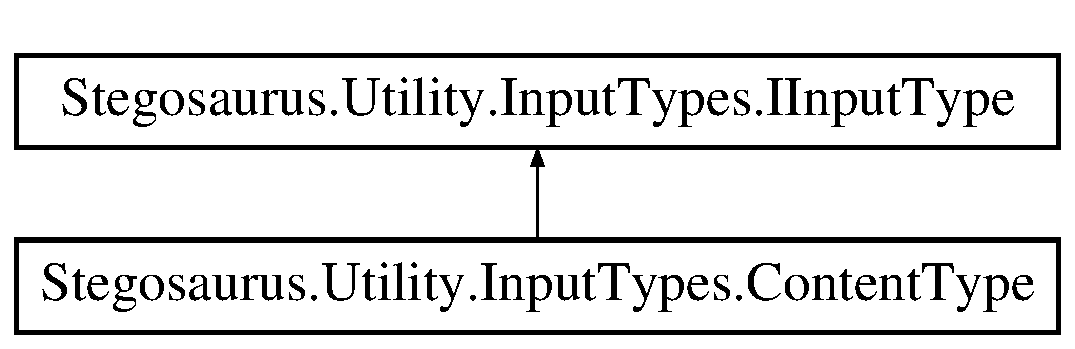
\includegraphics[height=2.000000cm]{class_stegosaurus_1_1_utility_1_1_input_types_1_1_content_type}
\end{center}
\end{figure}
\subsection*{Public Member Functions}
\begin{DoxyCompactItemize}
\item 
{\bfseries Content\+Type} (string \+\_\+file\+Path)\hypertarget{class_stegosaurus_1_1_utility_1_1_input_types_1_1_content_type_a4619d41d921c650970f52651fae597be}{}\label{class_stegosaurus_1_1_utility_1_1_input_types_1_1_content_type_a4619d41d921c650970f52651fae597be}

\end{DoxyCompactItemize}
\subsection*{Properties}
\begin{DoxyCompactItemize}
\item 
string {\bfseries File\+Path}\hspace{0.3cm}{\ttfamily  \mbox{[}get, set\mbox{]}}\hypertarget{class_stegosaurus_1_1_utility_1_1_input_types_1_1_content_type_a1dd896bd9805259e1294da3110b3f0a3}{}\label{class_stegosaurus_1_1_utility_1_1_input_types_1_1_content_type_a1dd896bd9805259e1294da3110b3f0a3}

\end{DoxyCompactItemize}


The documentation for this class was generated from the following file\+:\begin{DoxyCompactItemize}
\item 
Steganography/\+Stegosaurus/\+Utility/\+Input\+Types/Content\+Type.\+cs\end{DoxyCompactItemize}

\hypertarget{class_stegosaurus_1_1_extensions_1_1_input_extensions_1_1_content_type}{}\section{Stegosaurus.\+Extensions.\+Input\+Extensions.\+Content\+Type Class Reference}
\label{class_stegosaurus_1_1_extensions_1_1_input_extensions_1_1_content_type}\index{Stegosaurus.\+Extensions.\+Input\+Extensions.\+Content\+Type@{Stegosaurus.\+Extensions.\+Input\+Extensions.\+Content\+Type}}
Inheritance diagram for Stegosaurus.\+Extensions.\+Input\+Extensions.\+Content\+Type\+:\begin{figure}[H]
\begin{center}
\leavevmode
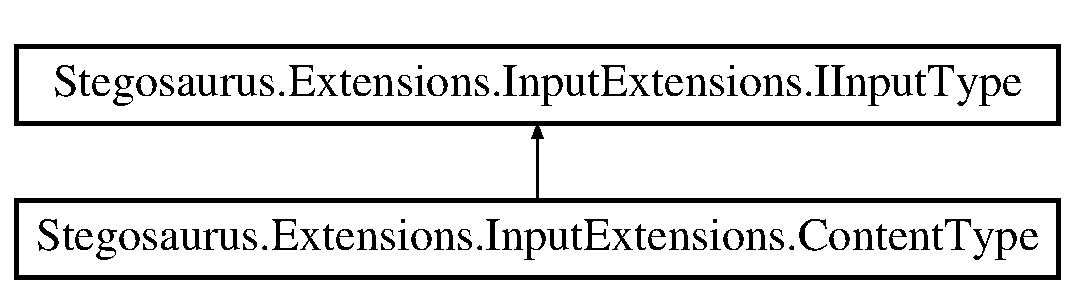
\includegraphics[height=2.000000cm]{class_stegosaurus_1_1_extensions_1_1_input_extensions_1_1_content_type}
\end{center}
\end{figure}
\subsection*{Public Member Functions}
\begin{DoxyCompactItemize}
\item 
{\bfseries Content\+Type} (string \+\_\+file\+Path)\hypertarget{class_stegosaurus_1_1_extensions_1_1_input_extensions_1_1_content_type_a4ec62e99c27424bf0e35a291442cd7c0}{}\label{class_stegosaurus_1_1_extensions_1_1_input_extensions_1_1_content_type_a4ec62e99c27424bf0e35a291442cd7c0}

\end{DoxyCompactItemize}
\subsection*{Properties}
\begin{DoxyCompactItemize}
\item 
string {\bfseries File\+Path}\hspace{0.3cm}{\ttfamily  \mbox{[}get, set\mbox{]}}\hypertarget{class_stegosaurus_1_1_extensions_1_1_input_extensions_1_1_content_type_a33511db053db12bf2742e48c752497af}{}\label{class_stegosaurus_1_1_extensions_1_1_input_extensions_1_1_content_type_a33511db053db12bf2742e48c752497af}

\end{DoxyCompactItemize}


The documentation for this class was generated from the following file\+:\begin{DoxyCompactItemize}
\item 
Steganography/\+Stegosaurus/\+Extensions/\+Input\+Extensions/Content\+Type.\+cs\end{DoxyCompactItemize}

\hypertarget{class_stegosaurus_1_1_algorithm_1_1_graph_theory_1_1_counted_vertice_list}{}\section{Stegosaurus.\+Algorithm.\+Graph\+Theory.\+Counted\+Vertice\+List Class Reference}
\label{class_stegosaurus_1_1_algorithm_1_1_graph_theory_1_1_counted_vertice_list}\index{Stegosaurus.\+Algorithm.\+Graph\+Theory.\+Counted\+Vertice\+List@{Stegosaurus.\+Algorithm.\+Graph\+Theory.\+Counted\+Vertice\+List}}
\subsection*{Public Member Functions}
\begin{DoxyCompactItemize}
\item 
void {\bfseries Add} (\hyperlink{class_stegosaurus_1_1_algorithm_1_1_graph_theory_1_1_vertex}{Vertex} \+\_\+new\+Vertex)\hypertarget{class_stegosaurus_1_1_algorithm_1_1_graph_theory_1_1_counted_vertice_list_a1f643243c256fb7c317954ec4bd0d29a}{}\label{class_stegosaurus_1_1_algorithm_1_1_graph_theory_1_1_counted_vertice_list_a1f643243c256fb7c317954ec4bd0d29a}

\item 
\hyperlink{class_stegosaurus_1_1_algorithm_1_1_graph_theory_1_1_vertex}{Vertex} {\bfseries Get} (int \+\_\+index)\hypertarget{class_stegosaurus_1_1_algorithm_1_1_graph_theory_1_1_counted_vertice_list_a67d04680ba06801c47bc45fc6456ea49}{}\label{class_stegosaurus_1_1_algorithm_1_1_graph_theory_1_1_counted_vertice_list_a67d04680ba06801c47bc45fc6456ea49}

\end{DoxyCompactItemize}
\subsection*{Public Attributes}
\begin{DoxyCompactItemize}
\item 
int {\bfseries Count} = 0\hypertarget{class_stegosaurus_1_1_algorithm_1_1_graph_theory_1_1_counted_vertice_list_a209a4a0877da2d127a2dbb769a22d929}{}\label{class_stegosaurus_1_1_algorithm_1_1_graph_theory_1_1_counted_vertice_list_a209a4a0877da2d127a2dbb769a22d929}

\item 
List$<$ \hyperlink{class_stegosaurus_1_1_algorithm_1_1_graph_theory_1_1_vertex}{Vertex} $>$ {\bfseries vertices} = new List$<$\hyperlink{class_stegosaurus_1_1_algorithm_1_1_graph_theory_1_1_vertex}{Vertex}$>$()\hypertarget{class_stegosaurus_1_1_algorithm_1_1_graph_theory_1_1_counted_vertice_list_a951306fa54af75dd02c6aad68601ddc2}{}\label{class_stegosaurus_1_1_algorithm_1_1_graph_theory_1_1_counted_vertice_list_a951306fa54af75dd02c6aad68601ddc2}

\end{DoxyCompactItemize}


The documentation for this class was generated from the following file\+:\begin{DoxyCompactItemize}
\item 
Steganography/\+Stegosaurus/\+Algorithm/\+Graph\+Theory/Counted\+Vertice\+List.\+cs\end{DoxyCompactItemize}

\hypertarget{class_stegosaurus_1_1_algorithm_1_1_graph_theory_1_1_edge}{}\section{Stegosaurus.\+Algorithm.\+Graph\+Theory.\+Edge Class Reference}
\label{class_stegosaurus_1_1_algorithm_1_1_graph_theory_1_1_edge}\index{Stegosaurus.\+Algorithm.\+Graph\+Theory.\+Edge@{Stegosaurus.\+Algorithm.\+Graph\+Theory.\+Edge}}
\subsection*{Public Member Functions}
\begin{DoxyCompactItemize}
\item 
{\bfseries Edge} (\hyperlink{class_stegosaurus_1_1_algorithm_1_1_graph_theory_1_1_vertex}{Vertex} \+\_\+first\+Vertex, \hyperlink{class_stegosaurus_1_1_algorithm_1_1_graph_theory_1_1_vertex}{Vertex} \+\_\+second\+Vertex, short \+\_\+weight, byte\mbox{[}$\,$\mbox{]} \+\_\+best\+Swaps)\hypertarget{class_stegosaurus_1_1_algorithm_1_1_graph_theory_1_1_edge_afe2a496b57a45d06fb4d91e00262d002}{}\label{class_stegosaurus_1_1_algorithm_1_1_graph_theory_1_1_edge_afe2a496b57a45d06fb4d91e00262d002}

\item 
override string {\bfseries To\+String} ()\hypertarget{class_stegosaurus_1_1_algorithm_1_1_graph_theory_1_1_edge_ae68712118b1092b43dc3c00d46de7650}{}\label{class_stegosaurus_1_1_algorithm_1_1_graph_theory_1_1_edge_ae68712118b1092b43dc3c00d46de7650}

\end{DoxyCompactItemize}
\subsection*{Public Attributes}
\begin{DoxyCompactItemize}
\item 
\hyperlink{class_stegosaurus_1_1_algorithm_1_1_graph_theory_1_1_vertex}{Vertex}\mbox{[}$\,$\mbox{]} {\bfseries Vertices} = new \hyperlink{class_stegosaurus_1_1_algorithm_1_1_graph_theory_1_1_vertex}{Vertex}\mbox{[}2\mbox{]}\hypertarget{class_stegosaurus_1_1_algorithm_1_1_graph_theory_1_1_edge_a2c0f28a278e329a7d64f2a74b0c98f6c}{}\label{class_stegosaurus_1_1_algorithm_1_1_graph_theory_1_1_edge_a2c0f28a278e329a7d64f2a74b0c98f6c}

\item 
short {\bfseries Weight}\hypertarget{class_stegosaurus_1_1_algorithm_1_1_graph_theory_1_1_edge_afd137dab2e9ab9c32e66f72e14900b5f}{}\label{class_stegosaurus_1_1_algorithm_1_1_graph_theory_1_1_edge_afd137dab2e9ab9c32e66f72e14900b5f}

\item 
byte\mbox{[}$\,$\mbox{]} {\bfseries Best\+Swaps}\hypertarget{class_stegosaurus_1_1_algorithm_1_1_graph_theory_1_1_edge_a9abebfba06f3aac63eef2dbd57e06886}{}\label{class_stegosaurus_1_1_algorithm_1_1_graph_theory_1_1_edge_a9abebfba06f3aac63eef2dbd57e06886}

\end{DoxyCompactItemize}


The documentation for this class was generated from the following file\+:\begin{DoxyCompactItemize}
\item 
Steganography/\+Stegosaurus/\+Algorithm/\+Graph\+Theory/Edge.\+cs\end{DoxyCompactItemize}

\hypertarget{class_stegosaurus_1_1_forms_1_1_form_embedding_progress}{}\section{Stegosaurus.\+Forms.\+Form\+Embedding\+Progress Class Reference}
\label{class_stegosaurus_1_1_forms_1_1_form_embedding_progress}\index{Stegosaurus.\+Forms.\+Form\+Embedding\+Progress@{Stegosaurus.\+Forms.\+Form\+Embedding\+Progress}}
Inheritance diagram for Stegosaurus.\+Forms.\+Form\+Embedding\+Progress\+:\begin{figure}[H]
\begin{center}
\leavevmode
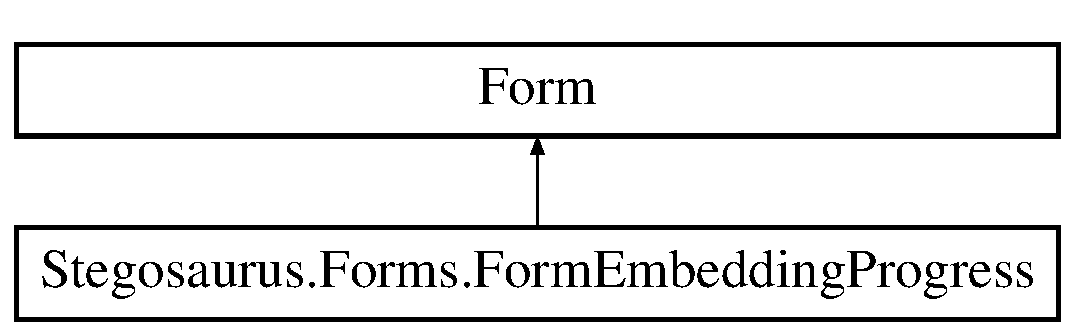
\includegraphics[height=2.000000cm]{class_stegosaurus_1_1_forms_1_1_form_embedding_progress}
\end{center}
\end{figure}
\subsection*{Public Member Functions}
\begin{DoxyCompactItemize}
\item 
async Task {\bfseries Run} (\hyperlink{class_stegosaurus_1_1_stego_message}{Stego\+Message} \+\_\+message, \hyperlink{class_stegosaurus_1_1_algorithm_1_1_stego_algorithm_base}{Stego\+Algorithm\+Base} \+\_\+algorithm, string \+\_\+name, string \+\_\+extension)\hypertarget{class_stegosaurus_1_1_forms_1_1_form_embedding_progress_af74aededc4f874344a835fd5f9666867}{}\label{class_stegosaurus_1_1_forms_1_1_form_embedding_progress_af74aededc4f874344a835fd5f9666867}

\end{DoxyCompactItemize}
\subsection*{Protected Member Functions}
\begin{DoxyCompactItemize}
\item 
override void \hyperlink{class_stegosaurus_1_1_forms_1_1_form_embedding_progress_ab0fd642aa396f03edcc0315891d963ff}{Dispose} (bool disposing)
\begin{DoxyCompactList}\small\item\em Clean up any resources being used. \end{DoxyCompactList}\end{DoxyCompactItemize}


\subsection{Member Function Documentation}
\index{Stegosaurus\+::\+Forms\+::\+Form\+Embedding\+Progress@{Stegosaurus\+::\+Forms\+::\+Form\+Embedding\+Progress}!Dispose@{Dispose}}
\index{Dispose@{Dispose}!Stegosaurus\+::\+Forms\+::\+Form\+Embedding\+Progress@{Stegosaurus\+::\+Forms\+::\+Form\+Embedding\+Progress}}
\subsubsection[{\texorpdfstring{Dispose(bool disposing)}{Dispose(bool disposing)}}]{\setlength{\rightskip}{0pt plus 5cm}override void Stegosaurus.\+Forms.\+Form\+Embedding\+Progress.\+Dispose (
\begin{DoxyParamCaption}
\item[{bool}]{disposing}
\end{DoxyParamCaption}
)\hspace{0.3cm}{\ttfamily [protected]}}\hypertarget{class_stegosaurus_1_1_forms_1_1_form_embedding_progress_ab0fd642aa396f03edcc0315891d963ff}{}\label{class_stegosaurus_1_1_forms_1_1_form_embedding_progress_ab0fd642aa396f03edcc0315891d963ff}


Clean up any resources being used. 


\begin{DoxyParams}{Parameters}
{\em disposing} & true if managed resources should be disposed; otherwise, false.\\
\hline
\end{DoxyParams}


The documentation for this class was generated from the following files\+:\begin{DoxyCompactItemize}
\item 
Steganography/\+Stegosaurus/\+Forms/Form\+Embedding\+Progress.\+cs\item 
Steganography/\+Stegosaurus/\+Forms/Form\+Embedding\+Progress.\+Designer.\+cs\end{DoxyCompactItemize}

\hypertarget{class_stegosaurus_1_1_forms_1_1_form_main}{}\section{Stegosaurus.\+Forms.\+Form\+Main Class Reference}
\label{class_stegosaurus_1_1_forms_1_1_form_main}\index{Stegosaurus.\+Forms.\+Form\+Main@{Stegosaurus.\+Forms.\+Form\+Main}}
Inheritance diagram for Stegosaurus.\+Forms.\+Form\+Main\+:\begin{figure}[H]
\begin{center}
\leavevmode
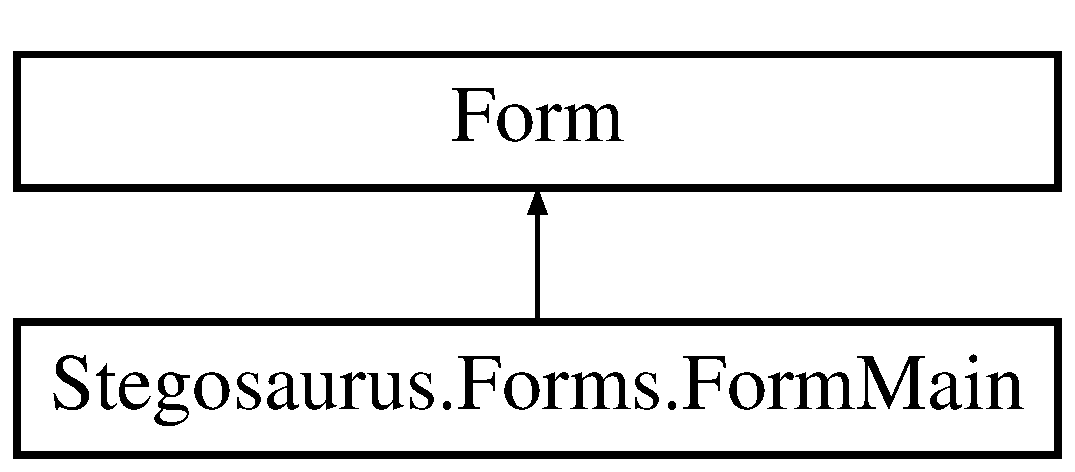
\includegraphics[height=2.000000cm]{class_stegosaurus_1_1_forms_1_1_form_main}
\end{center}
\end{figure}
\subsection*{Protected Member Functions}
\begin{DoxyCompactItemize}
\item 
override void \hyperlink{class_stegosaurus_1_1_forms_1_1_form_main_acc443f8d82df09136ebc503845086c82}{Dispose} (bool disposing)
\begin{DoxyCompactList}\small\item\em Clean up any resources being used. \end{DoxyCompactList}\end{DoxyCompactItemize}


\subsection{Member Function Documentation}
\index{Stegosaurus\+::\+Forms\+::\+Form\+Main@{Stegosaurus\+::\+Forms\+::\+Form\+Main}!Dispose@{Dispose}}
\index{Dispose@{Dispose}!Stegosaurus\+::\+Forms\+::\+Form\+Main@{Stegosaurus\+::\+Forms\+::\+Form\+Main}}
\subsubsection[{\texorpdfstring{Dispose(bool disposing)}{Dispose(bool disposing)}}]{\setlength{\rightskip}{0pt plus 5cm}override void Stegosaurus.\+Forms.\+Form\+Main.\+Dispose (
\begin{DoxyParamCaption}
\item[{bool}]{disposing}
\end{DoxyParamCaption}
)\hspace{0.3cm}{\ttfamily [protected]}}\hypertarget{class_stegosaurus_1_1_forms_1_1_form_main_acc443f8d82df09136ebc503845086c82}{}\label{class_stegosaurus_1_1_forms_1_1_form_main_acc443f8d82df09136ebc503845086c82}


Clean up any resources being used. 


\begin{DoxyParams}{Parameters}
{\em disposing} & true if managed resources should be disposed; otherwise, false.\\
\hline
\end{DoxyParams}


The documentation for this class was generated from the following files\+:\begin{DoxyCompactItemize}
\item 
Steganography/\+Stegosaurus/\+Forms/Form\+Main.\+cs\item 
Steganography/\+Stegosaurus/\+Forms/Form\+Main.\+Designer.\+cs\end{DoxyCompactItemize}

\hypertarget{class_stegosaurus_1_1_algorithm_1_1_graph_theoretic_algorithm}{}\section{Stegosaurus.\+Algorithm.\+Graph\+Theoretic\+Algorithm Class Reference}
\label{class_stegosaurus_1_1_algorithm_1_1_graph_theoretic_algorithm}\index{Stegosaurus.\+Algorithm.\+Graph\+Theoretic\+Algorithm@{Stegosaurus.\+Algorithm.\+Graph\+Theoretic\+Algorithm}}
Inheritance diagram for Stegosaurus.\+Algorithm.\+Graph\+Theoretic\+Algorithm\+:\begin{figure}[H]
\begin{center}
\leavevmode
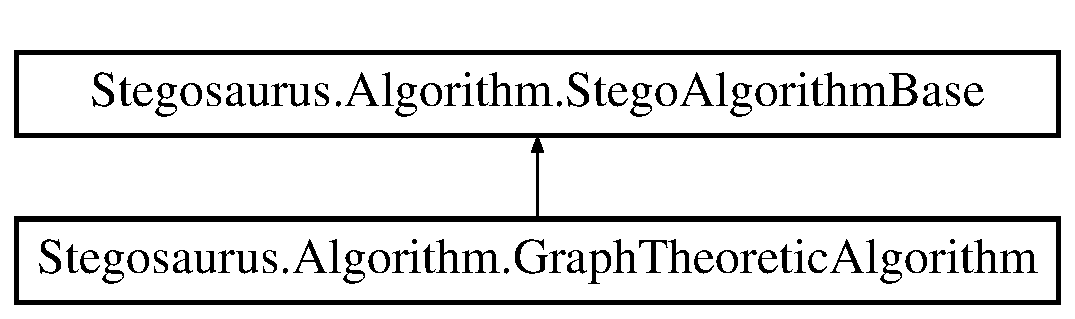
\includegraphics[height=2.000000cm]{class_stegosaurus_1_1_algorithm_1_1_graph_theoretic_algorithm}
\end{center}
\end{figure}
\subsection*{Public Member Functions}
\begin{DoxyCompactItemize}
\item 
override long \hyperlink{class_stegosaurus_1_1_algorithm_1_1_graph_theoretic_algorithm_aa3c0280792593fa75af74a7e3b9e8acc}{Compute\+Bandwidth} ()
\begin{DoxyCompactList}\small\item\em Returns the data capacity of the carrier media with the given algorithm. \end{DoxyCompactList}\item 
override void \hyperlink{class_stegosaurus_1_1_algorithm_1_1_graph_theoretic_algorithm_aecdce8aef6a5723d66bc93ca6f959767}{Embed} (\hyperlink{class_stegosaurus_1_1_stego_message}{Stego\+Message} \+\_\+message, I\+Progress$<$ int $>$ \+\_\+progress, Cancellation\+Token \+\_\+ct)
\begin{DoxyCompactList}\small\item\em Embeds a \hyperlink{class_stegosaurus_1_1_stego_message}{Stego\+Message} in the public Byte\+Array of the Carrier\+Media. \end{DoxyCompactList}\item 
override \hyperlink{class_stegosaurus_1_1_stego_message}{Stego\+Message} \hyperlink{class_stegosaurus_1_1_algorithm_1_1_graph_theoretic_algorithm_ae12e30f823e7cedc1f3ae75fa8a914fb}{Extract} ()
\begin{DoxyCompactList}\small\item\em Returns a \hyperlink{class_stegosaurus_1_1_stego_message}{Stego\+Message} by extracting from the public Byte\+Array of the Carrier\+Media. \end{DoxyCompactList}\end{DoxyCompactItemize}
\subsection*{Public Attributes}
\begin{DoxyCompactItemize}
\item 
override string {\bfseries Name} =$>$ \char`\"{}Graph Theoretic Algorithm\char`\"{}\hypertarget{class_stegosaurus_1_1_algorithm_1_1_graph_theoretic_algorithm_acfbd5778ddcb9cac2444625112727964}{}\label{class_stegosaurus_1_1_algorithm_1_1_graph_theoretic_algorithm_acfbd5778ddcb9cac2444625112727964}

\end{DoxyCompactItemize}
\subsection*{Properties}
\begin{DoxyCompactItemize}
\item 
byte {\bfseries Samples\+Per\+Vertex}\hspace{0.3cm}{\ttfamily  \mbox{[}get, set\mbox{]}}\hypertarget{class_stegosaurus_1_1_algorithm_1_1_graph_theoretic_algorithm_ab38113ed035bddf4d1ce6e9df5d3e2df}{}\label{class_stegosaurus_1_1_algorithm_1_1_graph_theoretic_algorithm_ab38113ed035bddf4d1ce6e9df5d3e2df}

\item 
byte {\bfseries Message\+Bits\+Per\+Vertex}\hspace{0.3cm}{\ttfamily  \mbox{[}get, set\mbox{]}}\hypertarget{class_stegosaurus_1_1_algorithm_1_1_graph_theoretic_algorithm_ab0c79fe6225f3b8e440945f2c45b895b}{}\label{class_stegosaurus_1_1_algorithm_1_1_graph_theoretic_algorithm_ab0c79fe6225f3b8e440945f2c45b895b}

\item 
ushort {\bfseries Discrimination\+Factor}\hspace{0.3cm}{\ttfamily  \mbox{[}get, set\mbox{]}}\hypertarget{class_stegosaurus_1_1_algorithm_1_1_graph_theoretic_algorithm_a93a75dad5e07d8887e92234fd83f3b99}{}\label{class_stegosaurus_1_1_algorithm_1_1_graph_theoretic_algorithm_a93a75dad5e07d8887e92234fd83f3b99}

\item 
override byte\mbox{[}$\,$\mbox{]} {\bfseries Signature}\hspace{0.3cm}{\ttfamily  \mbox{[}get\mbox{]}}\hypertarget{class_stegosaurus_1_1_algorithm_1_1_graph_theoretic_algorithm_ace57fbacebb4b718c842e750279789c9}{}\label{class_stegosaurus_1_1_algorithm_1_1_graph_theoretic_algorithm_ace57fbacebb4b718c842e750279789c9}

\end{DoxyCompactItemize}
\subsection*{Additional Inherited Members}


\subsection{Member Function Documentation}
\index{Stegosaurus\+::\+Algorithm\+::\+Graph\+Theoretic\+Algorithm@{Stegosaurus\+::\+Algorithm\+::\+Graph\+Theoretic\+Algorithm}!Compute\+Bandwidth@{Compute\+Bandwidth}}
\index{Compute\+Bandwidth@{Compute\+Bandwidth}!Stegosaurus\+::\+Algorithm\+::\+Graph\+Theoretic\+Algorithm@{Stegosaurus\+::\+Algorithm\+::\+Graph\+Theoretic\+Algorithm}}
\subsubsection[{\texorpdfstring{Compute\+Bandwidth()}{ComputeBandwidth()}}]{\setlength{\rightskip}{0pt plus 5cm}override long Stegosaurus.\+Algorithm.\+Graph\+Theoretic\+Algorithm.\+Compute\+Bandwidth (
\begin{DoxyParamCaption}
{}
\end{DoxyParamCaption}
)\hspace{0.3cm}{\ttfamily [virtual]}}\hypertarget{class_stegosaurus_1_1_algorithm_1_1_graph_theoretic_algorithm_aa3c0280792593fa75af74a7e3b9e8acc}{}\label{class_stegosaurus_1_1_algorithm_1_1_graph_theoretic_algorithm_aa3c0280792593fa75af74a7e3b9e8acc}


Returns the data capacity of the carrier media with the given algorithm. 



Implements \hyperlink{class_stegosaurus_1_1_algorithm_1_1_stego_algorithm_base_a2b4d2a0c3b65c980b5cbda2ab7601535}{Stegosaurus.\+Algorithm.\+Stego\+Algorithm\+Base}.

\index{Stegosaurus\+::\+Algorithm\+::\+Graph\+Theoretic\+Algorithm@{Stegosaurus\+::\+Algorithm\+::\+Graph\+Theoretic\+Algorithm}!Embed@{Embed}}
\index{Embed@{Embed}!Stegosaurus\+::\+Algorithm\+::\+Graph\+Theoretic\+Algorithm@{Stegosaurus\+::\+Algorithm\+::\+Graph\+Theoretic\+Algorithm}}
\subsubsection[{\texorpdfstring{Embed(\+Stego\+Message \+\_\+message, I\+Progress$<$ int $>$ \+\_\+progress, Cancellation\+Token \+\_\+ct)}{Embed(StegoMessage _message, IProgress< int > _progress, CancellationToken _ct)}}]{\setlength{\rightskip}{0pt plus 5cm}override void Stegosaurus.\+Algorithm.\+Graph\+Theoretic\+Algorithm.\+Embed (
\begin{DoxyParamCaption}
\item[{{\bf Stego\+Message}}]{\+\_\+message, }
\item[{I\+Progress$<$ int $>$}]{\+\_\+progress, }
\item[{Cancellation\+Token}]{\+\_\+ct}
\end{DoxyParamCaption}
)\hspace{0.3cm}{\ttfamily [virtual]}}\hypertarget{class_stegosaurus_1_1_algorithm_1_1_graph_theoretic_algorithm_aecdce8aef6a5723d66bc93ca6f959767}{}\label{class_stegosaurus_1_1_algorithm_1_1_graph_theoretic_algorithm_aecdce8aef6a5723d66bc93ca6f959767}


Embeds a \hyperlink{class_stegosaurus_1_1_stego_message}{Stego\+Message} in the public Byte\+Array of the Carrier\+Media. 



Implements \hyperlink{class_stegosaurus_1_1_algorithm_1_1_stego_algorithm_base_aa0d6b5f8f24d0ef5f9f2126b32cbad47}{Stegosaurus.\+Algorithm.\+Stego\+Algorithm\+Base}.

\index{Stegosaurus\+::\+Algorithm\+::\+Graph\+Theoretic\+Algorithm@{Stegosaurus\+::\+Algorithm\+::\+Graph\+Theoretic\+Algorithm}!Extract@{Extract}}
\index{Extract@{Extract}!Stegosaurus\+::\+Algorithm\+::\+Graph\+Theoretic\+Algorithm@{Stegosaurus\+::\+Algorithm\+::\+Graph\+Theoretic\+Algorithm}}
\subsubsection[{\texorpdfstring{Extract()}{Extract()}}]{\setlength{\rightskip}{0pt plus 5cm}override {\bf Stego\+Message} Stegosaurus.\+Algorithm.\+Graph\+Theoretic\+Algorithm.\+Extract (
\begin{DoxyParamCaption}
{}
\end{DoxyParamCaption}
)\hspace{0.3cm}{\ttfamily [virtual]}}\hypertarget{class_stegosaurus_1_1_algorithm_1_1_graph_theoretic_algorithm_ae12e30f823e7cedc1f3ae75fa8a914fb}{}\label{class_stegosaurus_1_1_algorithm_1_1_graph_theoretic_algorithm_ae12e30f823e7cedc1f3ae75fa8a914fb}


Returns a \hyperlink{class_stegosaurus_1_1_stego_message}{Stego\+Message} by extracting from the public Byte\+Array of the Carrier\+Media. 



Implements \hyperlink{class_stegosaurus_1_1_algorithm_1_1_stego_algorithm_base_a069eef0b17aa0221d2c111925b8d735a}{Stegosaurus.\+Algorithm.\+Stego\+Algorithm\+Base}.



The documentation for this class was generated from the following file\+:\begin{DoxyCompactItemize}
\item 
Steganography/\+Stegosaurus/\+Algorithm/Graph\+Theoretic\+Algorithm.\+cs\end{DoxyCompactItemize}

\hypertarget{interface_stegosaurus_1_1_carrier_1_1_i_carrier_media}{}\section{Stegosaurus.\+Carrier.\+I\+Carrier\+Media Interface Reference}
\label{interface_stegosaurus_1_1_carrier_1_1_i_carrier_media}\index{Stegosaurus.\+Carrier.\+I\+Carrier\+Media@{Stegosaurus.\+Carrier.\+I\+Carrier\+Media}}
Inheritance diagram for Stegosaurus.\+Carrier.\+I\+Carrier\+Media\+:\begin{figure}[H]
\begin{center}
\leavevmode
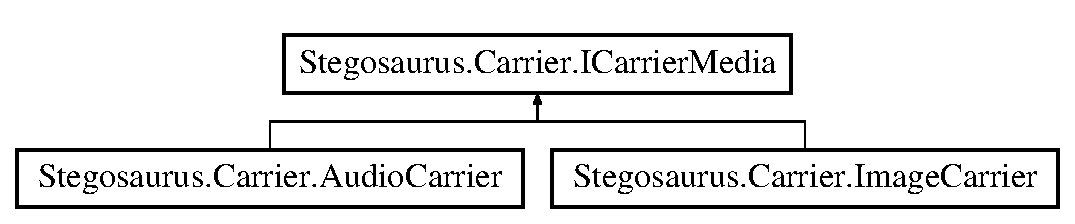
\includegraphics[height=2.000000cm]{interface_stegosaurus_1_1_carrier_1_1_i_carrier_media}
\end{center}
\end{figure}
\subsection*{Public Member Functions}
\begin{DoxyCompactItemize}
\item 
void \hyperlink{interface_stegosaurus_1_1_carrier_1_1_i_carrier_media_ac7d498eec146a74dbbaa2bd60e5bdce7}{Encode} ()
\begin{DoxyCompactList}\small\item\em Encodes Byte\+Array back into the carrier media. \end{DoxyCompactList}\item 
void \hyperlink{interface_stegosaurus_1_1_carrier_1_1_i_carrier_media_a863ecfa01ac50d9bb4a7619ce3f14fad}{Decode} ()
\begin{DoxyCompactList}\small\item\em Decodes the carrier media and sets Byte\+Array to the inner data. \end{DoxyCompactList}\item 
void \hyperlink{interface_stegosaurus_1_1_carrier_1_1_i_carrier_media_a419a6ed82dc1053f25e42a26e2fbade3}{Save\+To\+File} (string \+\_\+destination)
\begin{DoxyCompactList}\small\item\em Saves the carrier media to the specified destination. \end{DoxyCompactList}\end{DoxyCompactItemize}
\subsection*{Properties}
\begin{DoxyCompactItemize}
\item 
byte\mbox{[}$\,$\mbox{]} \hyperlink{interface_stegosaurus_1_1_carrier_1_1_i_carrier_media_a2ca3c8f4deb980992f5855c9c8653c91}{Byte\+Array}\hspace{0.3cm}{\ttfamily  \mbox{[}get, set\mbox{]}}
\begin{DoxyCompactList}\small\item\em The byte array containing samples of the carrier media. This array is to be used by algorithms. \end{DoxyCompactList}\item 
int \hyperlink{interface_stegosaurus_1_1_carrier_1_1_i_carrier_media_a53803a5166184ac2a6dc99000c3cbae6}{Bytes\+Per\+Sample}\hspace{0.3cm}{\ttfamily  \mbox{[}get\mbox{]}}
\begin{DoxyCompactList}\small\item\em The amount of bytes per sample, where a sample is defined as a sequence of bytes. For example, the pixels in an image are samples, where the amount of bytes is the amount of channels. \end{DoxyCompactList}\end{DoxyCompactItemize}


\subsection{Member Function Documentation}
\index{Stegosaurus\+::\+Carrier\+::\+I\+Carrier\+Media@{Stegosaurus\+::\+Carrier\+::\+I\+Carrier\+Media}!Decode@{Decode}}
\index{Decode@{Decode}!Stegosaurus\+::\+Carrier\+::\+I\+Carrier\+Media@{Stegosaurus\+::\+Carrier\+::\+I\+Carrier\+Media}}
\subsubsection[{\texorpdfstring{Decode()}{Decode()}}]{\setlength{\rightskip}{0pt plus 5cm}void Stegosaurus.\+Carrier.\+I\+Carrier\+Media.\+Decode (
\begin{DoxyParamCaption}
{}
\end{DoxyParamCaption}
)}\hypertarget{interface_stegosaurus_1_1_carrier_1_1_i_carrier_media_a863ecfa01ac50d9bb4a7619ce3f14fad}{}\label{interface_stegosaurus_1_1_carrier_1_1_i_carrier_media_a863ecfa01ac50d9bb4a7619ce3f14fad}


Decodes the carrier media and sets Byte\+Array to the inner data. 



Implemented in \hyperlink{class_stegosaurus_1_1_carrier_1_1_image_carrier_a1e22e324184654c3a81e0119dff2fd7a}{Stegosaurus.\+Carrier.\+Image\+Carrier}, and \hyperlink{class_stegosaurus_1_1_carrier_1_1_audio_carrier_a2d02a6c7c6ceda7a0a956ca2ab92a03d}{Stegosaurus.\+Carrier.\+Audio\+Carrier}.

\index{Stegosaurus\+::\+Carrier\+::\+I\+Carrier\+Media@{Stegosaurus\+::\+Carrier\+::\+I\+Carrier\+Media}!Encode@{Encode}}
\index{Encode@{Encode}!Stegosaurus\+::\+Carrier\+::\+I\+Carrier\+Media@{Stegosaurus\+::\+Carrier\+::\+I\+Carrier\+Media}}
\subsubsection[{\texorpdfstring{Encode()}{Encode()}}]{\setlength{\rightskip}{0pt plus 5cm}void Stegosaurus.\+Carrier.\+I\+Carrier\+Media.\+Encode (
\begin{DoxyParamCaption}
{}
\end{DoxyParamCaption}
)}\hypertarget{interface_stegosaurus_1_1_carrier_1_1_i_carrier_media_ac7d498eec146a74dbbaa2bd60e5bdce7}{}\label{interface_stegosaurus_1_1_carrier_1_1_i_carrier_media_ac7d498eec146a74dbbaa2bd60e5bdce7}


Encodes Byte\+Array back into the carrier media. 



Implemented in \hyperlink{class_stegosaurus_1_1_carrier_1_1_image_carrier_a0767501e55ca50a07641ca00b010dc7b}{Stegosaurus.\+Carrier.\+Image\+Carrier}, and \hyperlink{class_stegosaurus_1_1_carrier_1_1_audio_carrier_aacb57072610e4c5d59496d7e9c2262f0}{Stegosaurus.\+Carrier.\+Audio\+Carrier}.

\index{Stegosaurus\+::\+Carrier\+::\+I\+Carrier\+Media@{Stegosaurus\+::\+Carrier\+::\+I\+Carrier\+Media}!Save\+To\+File@{Save\+To\+File}}
\index{Save\+To\+File@{Save\+To\+File}!Stegosaurus\+::\+Carrier\+::\+I\+Carrier\+Media@{Stegosaurus\+::\+Carrier\+::\+I\+Carrier\+Media}}
\subsubsection[{\texorpdfstring{Save\+To\+File(string \+\_\+destination)}{SaveToFile(string _destination)}}]{\setlength{\rightskip}{0pt plus 5cm}void Stegosaurus.\+Carrier.\+I\+Carrier\+Media.\+Save\+To\+File (
\begin{DoxyParamCaption}
\item[{string}]{\+\_\+destination}
\end{DoxyParamCaption}
)}\hypertarget{interface_stegosaurus_1_1_carrier_1_1_i_carrier_media_a419a6ed82dc1053f25e42a26e2fbade3}{}\label{interface_stegosaurus_1_1_carrier_1_1_i_carrier_media_a419a6ed82dc1053f25e42a26e2fbade3}


Saves the carrier media to the specified destination. 



Implemented in \hyperlink{class_stegosaurus_1_1_carrier_1_1_image_carrier_a6a5a9c575f2ce202512fd99f6cabd0a3}{Stegosaurus.\+Carrier.\+Image\+Carrier}, and \hyperlink{class_stegosaurus_1_1_carrier_1_1_audio_carrier_ac703d4709853222c6dcc98d12f6c9130}{Stegosaurus.\+Carrier.\+Audio\+Carrier}.



\subsection{Property Documentation}
\index{Stegosaurus\+::\+Carrier\+::\+I\+Carrier\+Media@{Stegosaurus\+::\+Carrier\+::\+I\+Carrier\+Media}!Byte\+Array@{Byte\+Array}}
\index{Byte\+Array@{Byte\+Array}!Stegosaurus\+::\+Carrier\+::\+I\+Carrier\+Media@{Stegosaurus\+::\+Carrier\+::\+I\+Carrier\+Media}}
\subsubsection[{\texorpdfstring{Byte\+Array}{ByteArray}}]{\setlength{\rightskip}{0pt plus 5cm}byte \mbox{[}$\,$\mbox{]} Stegosaurus.\+Carrier.\+I\+Carrier\+Media.\+Byte\+Array\hspace{0.3cm}{\ttfamily [get]}, {\ttfamily [set]}}\hypertarget{interface_stegosaurus_1_1_carrier_1_1_i_carrier_media_a2ca3c8f4deb980992f5855c9c8653c91}{}\label{interface_stegosaurus_1_1_carrier_1_1_i_carrier_media_a2ca3c8f4deb980992f5855c9c8653c91}


The byte array containing samples of the carrier media. This array is to be used by algorithms. 

\index{Stegosaurus\+::\+Carrier\+::\+I\+Carrier\+Media@{Stegosaurus\+::\+Carrier\+::\+I\+Carrier\+Media}!Bytes\+Per\+Sample@{Bytes\+Per\+Sample}}
\index{Bytes\+Per\+Sample@{Bytes\+Per\+Sample}!Stegosaurus\+::\+Carrier\+::\+I\+Carrier\+Media@{Stegosaurus\+::\+Carrier\+::\+I\+Carrier\+Media}}
\subsubsection[{\texorpdfstring{Bytes\+Per\+Sample}{BytesPerSample}}]{\setlength{\rightskip}{0pt plus 5cm}int Stegosaurus.\+Carrier.\+I\+Carrier\+Media.\+Bytes\+Per\+Sample\hspace{0.3cm}{\ttfamily [get]}}\hypertarget{interface_stegosaurus_1_1_carrier_1_1_i_carrier_media_a53803a5166184ac2a6dc99000c3cbae6}{}\label{interface_stegosaurus_1_1_carrier_1_1_i_carrier_media_a53803a5166184ac2a6dc99000c3cbae6}


The amount of bytes per sample, where a sample is defined as a sequence of bytes. For example, the pixels in an image are samples, where the amount of bytes is the amount of channels. 



The documentation for this interface was generated from the following file\+:\begin{DoxyCompactItemize}
\item 
Steganography/\+Stegosaurus/\+Carrier/I\+Carrier\+Media.\+cs\end{DoxyCompactItemize}

\hypertarget{interface_stegosaurus_1_1_cryptography_1_1_i_crypto_provider}{}\section{Stegosaurus.\+Cryptography.\+I\+Crypto\+Provider Interface Reference}
\label{interface_stegosaurus_1_1_cryptography_1_1_i_crypto_provider}\index{Stegosaurus.\+Cryptography.\+I\+Crypto\+Provider@{Stegosaurus.\+Cryptography.\+I\+Crypto\+Provider}}
Inheritance diagram for Stegosaurus.\+Cryptography.\+I\+Crypto\+Provider\+:\begin{figure}[H]
\begin{center}
\leavevmode
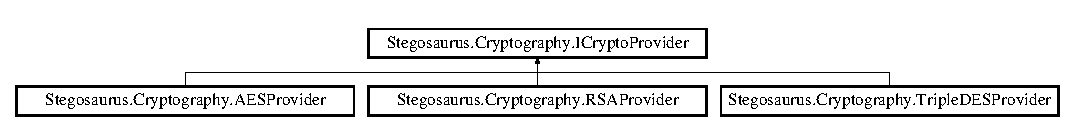
\includegraphics[height=1.323877cm]{interface_stegosaurus_1_1_cryptography_1_1_i_crypto_provider}
\end{center}
\end{figure}
\subsection*{Public Member Functions}
\begin{DoxyCompactItemize}
\item 
void \hyperlink{interface_stegosaurus_1_1_cryptography_1_1_i_crypto_provider_a95c1bb37e8bfdb62e6f66e8094d9d51b}{Set\+Key} (string \+\_\+key\+String)
\begin{DoxyCompactList}\small\item\em Set the Key from a string. \end{DoxyCompactList}\item 
byte\mbox{[}$\,$\mbox{]} \hyperlink{interface_stegosaurus_1_1_cryptography_1_1_i_crypto_provider_ae25c64411409f0cc41c2282030c6dc5c}{Generate\+Key} ()
\begin{DoxyCompactList}\small\item\em Generates and returns a key which can be used with the algorithm. \end{DoxyCompactList}\item 
byte\mbox{[}$\,$\mbox{]} \hyperlink{interface_stegosaurus_1_1_cryptography_1_1_i_crypto_provider_a2222231bf16ba92e8efc8d515943aacd}{Encrypt} (byte\mbox{[}$\,$\mbox{]} \+\_\+data)
\begin{DoxyCompactList}\small\item\em Encrypts and returns encrypted data. \end{DoxyCompactList}\item 
byte\mbox{[}$\,$\mbox{]} \hyperlink{interface_stegosaurus_1_1_cryptography_1_1_i_crypto_provider_a673607b0f3392591db9c647d2499f38d}{Decrypt} (byte\mbox{[}$\,$\mbox{]} \+\_\+data)
\begin{DoxyCompactList}\small\item\em Decrypts and returns decrypted data. \end{DoxyCompactList}\end{DoxyCompactItemize}
\subsection*{Properties}
\begin{DoxyCompactItemize}
\item 
byte\mbox{[}$\,$\mbox{]} \hyperlink{interface_stegosaurus_1_1_cryptography_1_1_i_crypto_provider_a0a8633906966fa70858e0762db3633af}{Key}\hspace{0.3cm}{\ttfamily  \mbox{[}get, set\mbox{]}}
\begin{DoxyCompactList}\small\item\em The key to be used, either in encryption or decryption. \end{DoxyCompactList}\item 
string \hyperlink{interface_stegosaurus_1_1_cryptography_1_1_i_crypto_provider_a9b2e3db9ac5f22d5c30d5f1877e18bbb}{Name}\hspace{0.3cm}{\ttfamily  \mbox{[}get\mbox{]}}
\begin{DoxyCompactList}\small\item\em The name of the algorithm. \end{DoxyCompactList}\item 
int \hyperlink{interface_stegosaurus_1_1_cryptography_1_1_i_crypto_provider_a0322f20ed8b9f630de3945fcd32e282e}{Key\+Size}\hspace{0.3cm}{\ttfamily  \mbox{[}get\mbox{]}}
\begin{DoxyCompactList}\small\item\em The maximum key size in bits. \end{DoxyCompactList}\item 
int \hyperlink{interface_stegosaurus_1_1_cryptography_1_1_i_crypto_provider_acbb21695dbfa48878dda20f5159bc60b}{Seed}\hspace{0.3cm}{\ttfamily  \mbox{[}get\mbox{]}}
\begin{DoxyCompactList}\small\item\em The seed to be optionally used by algorithms, typically a hash of the encryption key. If an implementation of \hyperlink{interface_stegosaurus_1_1_cryptography_1_1_i_crypto_provider}{I\+Crypto\+Provider} is assymetric, it should still provide a symmetric seed. \end{DoxyCompactList}\end{DoxyCompactItemize}


\subsection{Member Function Documentation}
\index{Stegosaurus\+::\+Cryptography\+::\+I\+Crypto\+Provider@{Stegosaurus\+::\+Cryptography\+::\+I\+Crypto\+Provider}!Decrypt@{Decrypt}}
\index{Decrypt@{Decrypt}!Stegosaurus\+::\+Cryptography\+::\+I\+Crypto\+Provider@{Stegosaurus\+::\+Cryptography\+::\+I\+Crypto\+Provider}}
\subsubsection[{\texorpdfstring{Decrypt(byte[] \+\_\+data)}{Decrypt(byte[] _data)}}]{\setlength{\rightskip}{0pt plus 5cm}byte \mbox{[}$\,$\mbox{]} Stegosaurus.\+Cryptography.\+I\+Crypto\+Provider.\+Decrypt (
\begin{DoxyParamCaption}
\item[{byte\mbox{[}$\,$\mbox{]}}]{\+\_\+data}
\end{DoxyParamCaption}
)}\hypertarget{interface_stegosaurus_1_1_cryptography_1_1_i_crypto_provider_a673607b0f3392591db9c647d2499f38d}{}\label{interface_stegosaurus_1_1_cryptography_1_1_i_crypto_provider_a673607b0f3392591db9c647d2499f38d}


Decrypts and returns decrypted data. 



Implemented in \hyperlink{class_stegosaurus_1_1_cryptography_1_1_a_e_s_provider_a7f9c88ceae0fb598224b04953ee70e0a}{Stegosaurus.\+Cryptography.\+A\+E\+S\+Provider}, \hyperlink{class_stegosaurus_1_1_cryptography_1_1_r_s_a_provider_ae5bf59d4baa636c5b3639cc24e240468}{Stegosaurus.\+Cryptography.\+R\+S\+A\+Provider}, and \hyperlink{class_stegosaurus_1_1_cryptography_1_1_triple_d_e_s_provider_aae9a3eb3f23e3c8995252d6f1184fd70}{Stegosaurus.\+Cryptography.\+Triple\+D\+E\+S\+Provider}.

\index{Stegosaurus\+::\+Cryptography\+::\+I\+Crypto\+Provider@{Stegosaurus\+::\+Cryptography\+::\+I\+Crypto\+Provider}!Encrypt@{Encrypt}}
\index{Encrypt@{Encrypt}!Stegosaurus\+::\+Cryptography\+::\+I\+Crypto\+Provider@{Stegosaurus\+::\+Cryptography\+::\+I\+Crypto\+Provider}}
\subsubsection[{\texorpdfstring{Encrypt(byte[] \+\_\+data)}{Encrypt(byte[] _data)}}]{\setlength{\rightskip}{0pt plus 5cm}byte \mbox{[}$\,$\mbox{]} Stegosaurus.\+Cryptography.\+I\+Crypto\+Provider.\+Encrypt (
\begin{DoxyParamCaption}
\item[{byte\mbox{[}$\,$\mbox{]}}]{\+\_\+data}
\end{DoxyParamCaption}
)}\hypertarget{interface_stegosaurus_1_1_cryptography_1_1_i_crypto_provider_a2222231bf16ba92e8efc8d515943aacd}{}\label{interface_stegosaurus_1_1_cryptography_1_1_i_crypto_provider_a2222231bf16ba92e8efc8d515943aacd}


Encrypts and returns encrypted data. 



Implemented in \hyperlink{class_stegosaurus_1_1_cryptography_1_1_r_s_a_provider_aa3b8f1d8c55043ca741b4ec3fd456836}{Stegosaurus.\+Cryptography.\+R\+S\+A\+Provider}, \hyperlink{class_stegosaurus_1_1_cryptography_1_1_triple_d_e_s_provider_a3af1ec710220cb696b1266d3317a4e79}{Stegosaurus.\+Cryptography.\+Triple\+D\+E\+S\+Provider}, and \hyperlink{class_stegosaurus_1_1_cryptography_1_1_a_e_s_provider_a81deb5da864b25f93810afbd8fc6449d}{Stegosaurus.\+Cryptography.\+A\+E\+S\+Provider}.

\index{Stegosaurus\+::\+Cryptography\+::\+I\+Crypto\+Provider@{Stegosaurus\+::\+Cryptography\+::\+I\+Crypto\+Provider}!Generate\+Key@{Generate\+Key}}
\index{Generate\+Key@{Generate\+Key}!Stegosaurus\+::\+Cryptography\+::\+I\+Crypto\+Provider@{Stegosaurus\+::\+Cryptography\+::\+I\+Crypto\+Provider}}
\subsubsection[{\texorpdfstring{Generate\+Key()}{GenerateKey()}}]{\setlength{\rightskip}{0pt plus 5cm}byte \mbox{[}$\,$\mbox{]} Stegosaurus.\+Cryptography.\+I\+Crypto\+Provider.\+Generate\+Key (
\begin{DoxyParamCaption}
{}
\end{DoxyParamCaption}
)}\hypertarget{interface_stegosaurus_1_1_cryptography_1_1_i_crypto_provider_ae25c64411409f0cc41c2282030c6dc5c}{}\label{interface_stegosaurus_1_1_cryptography_1_1_i_crypto_provider_ae25c64411409f0cc41c2282030c6dc5c}


Generates and returns a key which can be used with the algorithm. 



Implemented in \hyperlink{class_stegosaurus_1_1_cryptography_1_1_r_s_a_provider_abf0779c0e2d3d295385af554c1776bc5}{Stegosaurus.\+Cryptography.\+R\+S\+A\+Provider}, \hyperlink{class_stegosaurus_1_1_cryptography_1_1_a_e_s_provider_a0e14ad61f9e6bb0555f159e2008153ee}{Stegosaurus.\+Cryptography.\+A\+E\+S\+Provider}, and \hyperlink{class_stegosaurus_1_1_cryptography_1_1_triple_d_e_s_provider_a7ed750ce72bf9adf2e35887d0ab67db8}{Stegosaurus.\+Cryptography.\+Triple\+D\+E\+S\+Provider}.

\index{Stegosaurus\+::\+Cryptography\+::\+I\+Crypto\+Provider@{Stegosaurus\+::\+Cryptography\+::\+I\+Crypto\+Provider}!Set\+Key@{Set\+Key}}
\index{Set\+Key@{Set\+Key}!Stegosaurus\+::\+Cryptography\+::\+I\+Crypto\+Provider@{Stegosaurus\+::\+Cryptography\+::\+I\+Crypto\+Provider}}
\subsubsection[{\texorpdfstring{Set\+Key(string \+\_\+key\+String)}{SetKey(string _keyString)}}]{\setlength{\rightskip}{0pt plus 5cm}void Stegosaurus.\+Cryptography.\+I\+Crypto\+Provider.\+Set\+Key (
\begin{DoxyParamCaption}
\item[{string}]{\+\_\+key\+String}
\end{DoxyParamCaption}
)}\hypertarget{interface_stegosaurus_1_1_cryptography_1_1_i_crypto_provider_a95c1bb37e8bfdb62e6f66e8094d9d51b}{}\label{interface_stegosaurus_1_1_cryptography_1_1_i_crypto_provider_a95c1bb37e8bfdb62e6f66e8094d9d51b}


Set the Key from a string. 



Implemented in \hyperlink{class_stegosaurus_1_1_cryptography_1_1_r_s_a_provider_a18053ea1b1d9709c8631e97bef06c6a8}{Stegosaurus.\+Cryptography.\+R\+S\+A\+Provider}, \hyperlink{class_stegosaurus_1_1_cryptography_1_1_a_e_s_provider_ab9119737779ce4aea6c8c7e6c4725923}{Stegosaurus.\+Cryptography.\+A\+E\+S\+Provider}, and \hyperlink{class_stegosaurus_1_1_cryptography_1_1_triple_d_e_s_provider_ab7413df54e7753ae7ce4776f94521c7a}{Stegosaurus.\+Cryptography.\+Triple\+D\+E\+S\+Provider}.



\subsection{Property Documentation}
\index{Stegosaurus\+::\+Cryptography\+::\+I\+Crypto\+Provider@{Stegosaurus\+::\+Cryptography\+::\+I\+Crypto\+Provider}!Key@{Key}}
\index{Key@{Key}!Stegosaurus\+::\+Cryptography\+::\+I\+Crypto\+Provider@{Stegosaurus\+::\+Cryptography\+::\+I\+Crypto\+Provider}}
\subsubsection[{\texorpdfstring{Key}{Key}}]{\setlength{\rightskip}{0pt plus 5cm}byte \mbox{[}$\,$\mbox{]} Stegosaurus.\+Cryptography.\+I\+Crypto\+Provider.\+Key\hspace{0.3cm}{\ttfamily [get]}, {\ttfamily [set]}}\hypertarget{interface_stegosaurus_1_1_cryptography_1_1_i_crypto_provider_a0a8633906966fa70858e0762db3633af}{}\label{interface_stegosaurus_1_1_cryptography_1_1_i_crypto_provider_a0a8633906966fa70858e0762db3633af}


The key to be used, either in encryption or decryption. 

\index{Stegosaurus\+::\+Cryptography\+::\+I\+Crypto\+Provider@{Stegosaurus\+::\+Cryptography\+::\+I\+Crypto\+Provider}!Key\+Size@{Key\+Size}}
\index{Key\+Size@{Key\+Size}!Stegosaurus\+::\+Cryptography\+::\+I\+Crypto\+Provider@{Stegosaurus\+::\+Cryptography\+::\+I\+Crypto\+Provider}}
\subsubsection[{\texorpdfstring{Key\+Size}{KeySize}}]{\setlength{\rightskip}{0pt plus 5cm}int Stegosaurus.\+Cryptography.\+I\+Crypto\+Provider.\+Key\+Size\hspace{0.3cm}{\ttfamily [get]}}\hypertarget{interface_stegosaurus_1_1_cryptography_1_1_i_crypto_provider_a0322f20ed8b9f630de3945fcd32e282e}{}\label{interface_stegosaurus_1_1_cryptography_1_1_i_crypto_provider_a0322f20ed8b9f630de3945fcd32e282e}


The maximum key size in bits. 

\index{Stegosaurus\+::\+Cryptography\+::\+I\+Crypto\+Provider@{Stegosaurus\+::\+Cryptography\+::\+I\+Crypto\+Provider}!Name@{Name}}
\index{Name@{Name}!Stegosaurus\+::\+Cryptography\+::\+I\+Crypto\+Provider@{Stegosaurus\+::\+Cryptography\+::\+I\+Crypto\+Provider}}
\subsubsection[{\texorpdfstring{Name}{Name}}]{\setlength{\rightskip}{0pt plus 5cm}string Stegosaurus.\+Cryptography.\+I\+Crypto\+Provider.\+Name\hspace{0.3cm}{\ttfamily [get]}}\hypertarget{interface_stegosaurus_1_1_cryptography_1_1_i_crypto_provider_a9b2e3db9ac5f22d5c30d5f1877e18bbb}{}\label{interface_stegosaurus_1_1_cryptography_1_1_i_crypto_provider_a9b2e3db9ac5f22d5c30d5f1877e18bbb}


The name of the algorithm. 

\index{Stegosaurus\+::\+Cryptography\+::\+I\+Crypto\+Provider@{Stegosaurus\+::\+Cryptography\+::\+I\+Crypto\+Provider}!Seed@{Seed}}
\index{Seed@{Seed}!Stegosaurus\+::\+Cryptography\+::\+I\+Crypto\+Provider@{Stegosaurus\+::\+Cryptography\+::\+I\+Crypto\+Provider}}
\subsubsection[{\texorpdfstring{Seed}{Seed}}]{\setlength{\rightskip}{0pt plus 5cm}int Stegosaurus.\+Cryptography.\+I\+Crypto\+Provider.\+Seed\hspace{0.3cm}{\ttfamily [get]}}\hypertarget{interface_stegosaurus_1_1_cryptography_1_1_i_crypto_provider_acbb21695dbfa48878dda20f5159bc60b}{}\label{interface_stegosaurus_1_1_cryptography_1_1_i_crypto_provider_acbb21695dbfa48878dda20f5159bc60b}


The seed to be optionally used by algorithms, typically a hash of the encryption key. If an implementation of \hyperlink{interface_stegosaurus_1_1_cryptography_1_1_i_crypto_provider}{I\+Crypto\+Provider} is assymetric, it should still provide a symmetric seed. 



The documentation for this interface was generated from the following file\+:\begin{DoxyCompactItemize}
\item 
Steganography/\+Stegosaurus/\+Cryptography/I\+Crypto\+Provider.\+cs\end{DoxyCompactItemize}

\hypertarget{interface_stegosaurus_1_1_utility_1_1_input_types_1_1_i_input_type}{}\section{Stegosaurus.\+Utility.\+Input\+Types.\+I\+Input\+Type Interface Reference}
\label{interface_stegosaurus_1_1_utility_1_1_input_types_1_1_i_input_type}\index{Stegosaurus.\+Utility.\+Input\+Types.\+I\+Input\+Type@{Stegosaurus.\+Utility.\+Input\+Types.\+I\+Input\+Type}}
Inheritance diagram for Stegosaurus.\+Utility.\+Input\+Types.\+I\+Input\+Type\+:\begin{figure}[H]
\begin{center}
\leavevmode
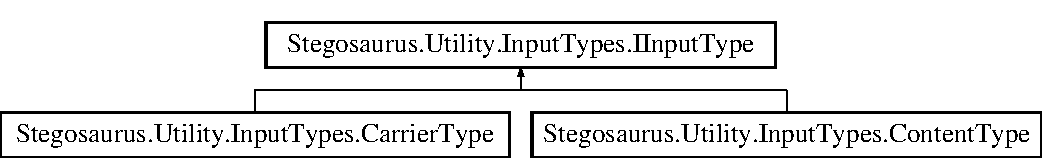
\includegraphics[height=2.000000cm]{interface_stegosaurus_1_1_utility_1_1_input_types_1_1_i_input_type}
\end{center}
\end{figure}
\subsection*{Properties}
\begin{DoxyCompactItemize}
\item 
string {\bfseries File\+Path}\hspace{0.3cm}{\ttfamily  \mbox{[}get, set\mbox{]}}\hypertarget{interface_stegosaurus_1_1_utility_1_1_input_types_1_1_i_input_type_a629965c94aabed5498436317cf4a67ff}{}\label{interface_stegosaurus_1_1_utility_1_1_input_types_1_1_i_input_type_a629965c94aabed5498436317cf4a67ff}

\end{DoxyCompactItemize}


The documentation for this interface was generated from the following file\+:\begin{DoxyCompactItemize}
\item 
Steganography/\+Stegosaurus/\+Utility/\+Input\+Types/I\+Input\+Type.\+cs\end{DoxyCompactItemize}

\hypertarget{interface_stegosaurus_1_1_extensions_1_1_input_extensions_1_1_i_input_type}{}\section{Stegosaurus.\+Extensions.\+Input\+Extensions.\+I\+Input\+Type Interface Reference}
\label{interface_stegosaurus_1_1_extensions_1_1_input_extensions_1_1_i_input_type}\index{Stegosaurus.\+Extensions.\+Input\+Extensions.\+I\+Input\+Type@{Stegosaurus.\+Extensions.\+Input\+Extensions.\+I\+Input\+Type}}
Inheritance diagram for Stegosaurus.\+Extensions.\+Input\+Extensions.\+I\+Input\+Type\+:\begin{figure}[H]
\begin{center}
\leavevmode
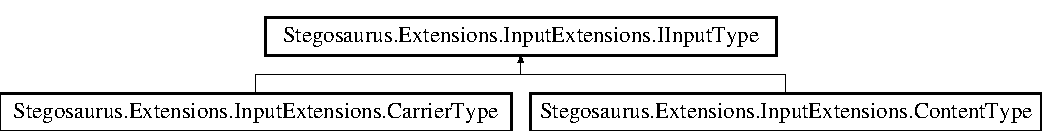
\includegraphics[height=1.750000cm]{interface_stegosaurus_1_1_extensions_1_1_input_extensions_1_1_i_input_type}
\end{center}
\end{figure}
\subsection*{Properties}
\begin{DoxyCompactItemize}
\item 
string {\bfseries File\+Path}\hspace{0.3cm}{\ttfamily  \mbox{[}get, set\mbox{]}}\hypertarget{interface_stegosaurus_1_1_extensions_1_1_input_extensions_1_1_i_input_type_ac8dccdd490b4fc15c965eca275858476}{}\label{interface_stegosaurus_1_1_extensions_1_1_input_extensions_1_1_i_input_type_ac8dccdd490b4fc15c965eca275858476}

\end{DoxyCompactItemize}


The documentation for this interface was generated from the following file\+:\begin{DoxyCompactItemize}
\item 
Steganography/\+Stegosaurus/\+Extensions/\+Input\+Extensions/I\+Input\+Type.\+cs\end{DoxyCompactItemize}

\hypertarget{class_stegosaurus_1_1_carrier_1_1_image_carrier}{}\section{Stegosaurus.\+Carrier.\+Image\+Carrier Class Reference}
\label{class_stegosaurus_1_1_carrier_1_1_image_carrier}\index{Stegosaurus.\+Carrier.\+Image\+Carrier@{Stegosaurus.\+Carrier.\+Image\+Carrier}}
Inheritance diagram for Stegosaurus.\+Carrier.\+Image\+Carrier\+:\begin{figure}[H]
\begin{center}
\leavevmode
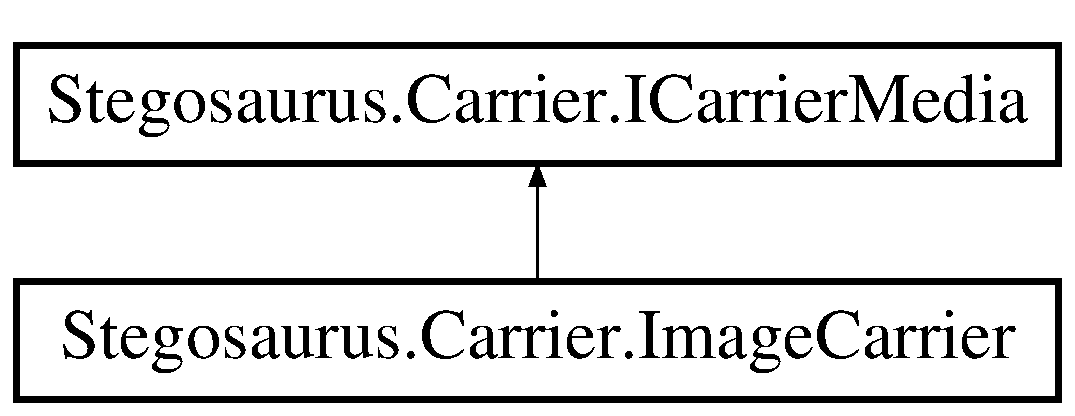
\includegraphics[height=2.000000cm]{class_stegosaurus_1_1_carrier_1_1_image_carrier}
\end{center}
\end{figure}
\subsection*{Public Member Functions}
\begin{DoxyCompactItemize}
\item 
\hyperlink{class_stegosaurus_1_1_carrier_1_1_image_carrier_af33775a68bd7a235779bd102ade02e27}{Image\+Carrier} (\hyperlink{class_stegosaurus_1_1_carrier_1_1_image_carrier_a75c34608afe89054cf1de0729d37f5ac}{Image} \+\_\+image)
\begin{DoxyCompactList}\small\item\em Construct \hyperlink{class_stegosaurus_1_1_carrier_1_1_image_carrier}{Image\+Carrier} from an instance of Image. \end{DoxyCompactList}\item 
\hyperlink{class_stegosaurus_1_1_carrier_1_1_image_carrier_a1729846d0a60c69f86a2c9ef1fe85fbe}{Image\+Carrier} (string \+\_\+file\+Path)
\begin{DoxyCompactList}\small\item\em Gets file path to image file and passes instace of Image to constructor. \end{DoxyCompactList}\item 
void \hyperlink{class_stegosaurus_1_1_carrier_1_1_image_carrier_a1e22e324184654c3a81e0119dff2fd7a}{Decode} ()
\begin{DoxyCompactList}\small\item\em Decodes the carrier media and sets Byte\+Array to the inner data. \end{DoxyCompactList}\item 
void \hyperlink{class_stegosaurus_1_1_carrier_1_1_image_carrier_a0767501e55ca50a07641ca00b010dc7b}{Encode} ()
\begin{DoxyCompactList}\small\item\em Moves data from Byte\+Array into inner\+Image. \end{DoxyCompactList}\item 
void \hyperlink{class_stegosaurus_1_1_carrier_1_1_image_carrier_a6a5a9c575f2ce202512fd99f6cabd0a3}{Save\+To\+File} (string \+\_\+destination)
\begin{DoxyCompactList}\small\item\em Encodes and saves file to destination. \end{DoxyCompactList}\end{DoxyCompactItemize}
\subsection*{Public Attributes}
\begin{DoxyCompactItemize}
\item 
int {\bfseries Bytes\+Per\+Sample} =$>$ 3\hypertarget{class_stegosaurus_1_1_carrier_1_1_image_carrier_a3baec8e258b4d043329a3402814f35a3}{}\label{class_stegosaurus_1_1_carrier_1_1_image_carrier_a3baec8e258b4d043329a3402814f35a3}

\item 
Image \hyperlink{class_stegosaurus_1_1_carrier_1_1_image_carrier_a75c34608afe89054cf1de0729d37f5ac}{Image} =$>$ image
\begin{DoxyCompactList}\small\item\em Returns the inner instance of Image. \end{DoxyCompactList}\end{DoxyCompactItemize}
\subsection*{Properties}
\begin{DoxyCompactItemize}
\item 
byte\mbox{[}$\,$\mbox{]} {\bfseries Byte\+Array}\hspace{0.3cm}{\ttfamily  \mbox{[}get, set\mbox{]}}\hypertarget{class_stegosaurus_1_1_carrier_1_1_image_carrier_af9508fc6e02ba3c5b9b58bc34ec8a228}{}\label{class_stegosaurus_1_1_carrier_1_1_image_carrier_af9508fc6e02ba3c5b9b58bc34ec8a228}

\end{DoxyCompactItemize}


\subsection{Constructor \& Destructor Documentation}
\index{Stegosaurus\+::\+Carrier\+::\+Image\+Carrier@{Stegosaurus\+::\+Carrier\+::\+Image\+Carrier}!Image\+Carrier@{Image\+Carrier}}
\index{Image\+Carrier@{Image\+Carrier}!Stegosaurus\+::\+Carrier\+::\+Image\+Carrier@{Stegosaurus\+::\+Carrier\+::\+Image\+Carrier}}
\subsubsection[{\texorpdfstring{Image\+Carrier(\+Image \+\_\+image)}{ImageCarrier(Image _image)}}]{\setlength{\rightskip}{0pt plus 5cm}Stegosaurus.\+Carrier.\+Image\+Carrier.\+Image\+Carrier (
\begin{DoxyParamCaption}
\item[{{\bf Image}}]{\+\_\+image}
\end{DoxyParamCaption}
)}\hypertarget{class_stegosaurus_1_1_carrier_1_1_image_carrier_af33775a68bd7a235779bd102ade02e27}{}\label{class_stegosaurus_1_1_carrier_1_1_image_carrier_af33775a68bd7a235779bd102ade02e27}


Construct \hyperlink{class_stegosaurus_1_1_carrier_1_1_image_carrier}{Image\+Carrier} from an instance of Image. 

\index{Stegosaurus\+::\+Carrier\+::\+Image\+Carrier@{Stegosaurus\+::\+Carrier\+::\+Image\+Carrier}!Image\+Carrier@{Image\+Carrier}}
\index{Image\+Carrier@{Image\+Carrier}!Stegosaurus\+::\+Carrier\+::\+Image\+Carrier@{Stegosaurus\+::\+Carrier\+::\+Image\+Carrier}}
\subsubsection[{\texorpdfstring{Image\+Carrier(string \+\_\+file\+Path)}{ImageCarrier(string _filePath)}}]{\setlength{\rightskip}{0pt plus 5cm}Stegosaurus.\+Carrier.\+Image\+Carrier.\+Image\+Carrier (
\begin{DoxyParamCaption}
\item[{string}]{\+\_\+file\+Path}
\end{DoxyParamCaption}
)}\hypertarget{class_stegosaurus_1_1_carrier_1_1_image_carrier_a1729846d0a60c69f86a2c9ef1fe85fbe}{}\label{class_stegosaurus_1_1_carrier_1_1_image_carrier_a1729846d0a60c69f86a2c9ef1fe85fbe}


Gets file path to image file and passes instace of Image to constructor. 


\begin{DoxyParams}{Parameters}
{\em \+\_\+file\+Path} & \\
\hline
\end{DoxyParams}


\subsection{Member Function Documentation}
\index{Stegosaurus\+::\+Carrier\+::\+Image\+Carrier@{Stegosaurus\+::\+Carrier\+::\+Image\+Carrier}!Decode@{Decode}}
\index{Decode@{Decode}!Stegosaurus\+::\+Carrier\+::\+Image\+Carrier@{Stegosaurus\+::\+Carrier\+::\+Image\+Carrier}}
\subsubsection[{\texorpdfstring{Decode()}{Decode()}}]{\setlength{\rightskip}{0pt plus 5cm}void Stegosaurus.\+Carrier.\+Image\+Carrier.\+Decode (
\begin{DoxyParamCaption}
{}
\end{DoxyParamCaption}
)}\hypertarget{class_stegosaurus_1_1_carrier_1_1_image_carrier_a1e22e324184654c3a81e0119dff2fd7a}{}\label{class_stegosaurus_1_1_carrier_1_1_image_carrier_a1e22e324184654c3a81e0119dff2fd7a}


Decodes the carrier media and sets Byte\+Array to the inner data. 



Implements \hyperlink{interface_stegosaurus_1_1_carrier_1_1_i_carrier_media_a863ecfa01ac50d9bb4a7619ce3f14fad}{Stegosaurus.\+Carrier.\+I\+Carrier\+Media}.

\index{Stegosaurus\+::\+Carrier\+::\+Image\+Carrier@{Stegosaurus\+::\+Carrier\+::\+Image\+Carrier}!Encode@{Encode}}
\index{Encode@{Encode}!Stegosaurus\+::\+Carrier\+::\+Image\+Carrier@{Stegosaurus\+::\+Carrier\+::\+Image\+Carrier}}
\subsubsection[{\texorpdfstring{Encode()}{Encode()}}]{\setlength{\rightskip}{0pt plus 5cm}void Stegosaurus.\+Carrier.\+Image\+Carrier.\+Encode (
\begin{DoxyParamCaption}
{}
\end{DoxyParamCaption}
)}\hypertarget{class_stegosaurus_1_1_carrier_1_1_image_carrier_a0767501e55ca50a07641ca00b010dc7b}{}\label{class_stegosaurus_1_1_carrier_1_1_image_carrier_a0767501e55ca50a07641ca00b010dc7b}


Moves data from Byte\+Array into inner\+Image. 



Implements \hyperlink{interface_stegosaurus_1_1_carrier_1_1_i_carrier_media_ac7d498eec146a74dbbaa2bd60e5bdce7}{Stegosaurus.\+Carrier.\+I\+Carrier\+Media}.

\index{Stegosaurus\+::\+Carrier\+::\+Image\+Carrier@{Stegosaurus\+::\+Carrier\+::\+Image\+Carrier}!Save\+To\+File@{Save\+To\+File}}
\index{Save\+To\+File@{Save\+To\+File}!Stegosaurus\+::\+Carrier\+::\+Image\+Carrier@{Stegosaurus\+::\+Carrier\+::\+Image\+Carrier}}
\subsubsection[{\texorpdfstring{Save\+To\+File(string \+\_\+destination)}{SaveToFile(string _destination)}}]{\setlength{\rightskip}{0pt plus 5cm}void Stegosaurus.\+Carrier.\+Image\+Carrier.\+Save\+To\+File (
\begin{DoxyParamCaption}
\item[{string}]{\+\_\+destination}
\end{DoxyParamCaption}
)}\hypertarget{class_stegosaurus_1_1_carrier_1_1_image_carrier_a6a5a9c575f2ce202512fd99f6cabd0a3}{}\label{class_stegosaurus_1_1_carrier_1_1_image_carrier_a6a5a9c575f2ce202512fd99f6cabd0a3}


Encodes and saves file to destination. 



Implements \hyperlink{interface_stegosaurus_1_1_carrier_1_1_i_carrier_media_a419a6ed82dc1053f25e42a26e2fbade3}{Stegosaurus.\+Carrier.\+I\+Carrier\+Media}.



\subsection{Member Data Documentation}
\index{Stegosaurus\+::\+Carrier\+::\+Image\+Carrier@{Stegosaurus\+::\+Carrier\+::\+Image\+Carrier}!Image@{Image}}
\index{Image@{Image}!Stegosaurus\+::\+Carrier\+::\+Image\+Carrier@{Stegosaurus\+::\+Carrier\+::\+Image\+Carrier}}
\subsubsection[{\texorpdfstring{Image}{Image}}]{\setlength{\rightskip}{0pt plus 5cm}Image Stegosaurus.\+Carrier.\+Image\+Carrier.\+Image =$>$ image}\hypertarget{class_stegosaurus_1_1_carrier_1_1_image_carrier_a75c34608afe89054cf1de0729d37f5ac}{}\label{class_stegosaurus_1_1_carrier_1_1_image_carrier_a75c34608afe89054cf1de0729d37f5ac}


Returns the inner instance of Image. 



The documentation for this class was generated from the following file\+:\begin{DoxyCompactItemize}
\item 
Steganography/\+Stegosaurus/\+Carrier/Image\+Carrier.\+cs\end{DoxyCompactItemize}

\hypertarget{class_stegosaurus_1_1_input_file}{}\section{Stegosaurus.\+Input\+File Class Reference}
\label{class_stegosaurus_1_1_input_file}\index{Stegosaurus.\+Input\+File@{Stegosaurus.\+Input\+File}}
\subsection*{Public Member Functions}
\begin{DoxyCompactItemize}
\item 
\hyperlink{class_stegosaurus_1_1_input_file_aa4a7db1edd50bbaf9a1375a0f1bf36f8}{Input\+File} (string \+\_\+name, byte\mbox{[}$\,$\mbox{]} \+\_\+content)
\begin{DoxyCompactList}\small\item\em A constructor to construct a \hyperlink{class_stegosaurus_1_1_input_file}{Input\+File} from byte array. \end{DoxyCompactList}\item 
\hyperlink{class_stegosaurus_1_1_input_file_ad06fe6aaf4a64d4e04abbef2492e06f3}{Input\+File} (string \+\_\+file\+Path)
\begin{DoxyCompactList}\small\item\em A constructor to construct a \hyperlink{class_stegosaurus_1_1_input_file}{Input\+File} from a file path. \end{DoxyCompactList}\item 
void \hyperlink{class_stegosaurus_1_1_input_file_a112c200323ceb421832cbbe882b512fb}{Save\+To} (string \+\_\+destination)
\begin{DoxyCompactList}\small\item\em This method is used to save the file in the file system of the operating system. \end{DoxyCompactList}\end{DoxyCompactItemize}
\subsection*{Properties}
\begin{DoxyCompactItemize}
\item 
string \hyperlink{class_stegosaurus_1_1_input_file_a02b6ebb5b60aa2f2b28a79a8ba386202}{Name}\hspace{0.3cm}{\ttfamily  \mbox{[}get\mbox{]}}
\begin{DoxyCompactList}\small\item\em The name of the file. \end{DoxyCompactList}\item 
byte\mbox{[}$\,$\mbox{]} \hyperlink{class_stegosaurus_1_1_input_file_ad83ede306bf1084b6724f254cec7661e}{Content}\hspace{0.3cm}{\ttfamily  \mbox{[}get\mbox{]}}
\begin{DoxyCompactList}\small\item\em A byte array containing the files contents. \end{DoxyCompactList}\end{DoxyCompactItemize}


\subsection{Constructor \& Destructor Documentation}
\index{Stegosaurus\+::\+Input\+File@{Stegosaurus\+::\+Input\+File}!Input\+File@{Input\+File}}
\index{Input\+File@{Input\+File}!Stegosaurus\+::\+Input\+File@{Stegosaurus\+::\+Input\+File}}
\subsubsection[{\texorpdfstring{Input\+File(string \+\_\+name, byte[] \+\_\+content)}{InputFile(string _name, byte[] _content)}}]{\setlength{\rightskip}{0pt plus 5cm}Stegosaurus.\+Input\+File.\+Input\+File (
\begin{DoxyParamCaption}
\item[{string}]{\+\_\+name, }
\item[{byte\mbox{[}$\,$\mbox{]}}]{\+\_\+content}
\end{DoxyParamCaption}
)}\hypertarget{class_stegosaurus_1_1_input_file_aa4a7db1edd50bbaf9a1375a0f1bf36f8}{}\label{class_stegosaurus_1_1_input_file_aa4a7db1edd50bbaf9a1375a0f1bf36f8}


A constructor to construct a \hyperlink{class_stegosaurus_1_1_input_file}{Input\+File} from byte array. 

\index{Stegosaurus\+::\+Input\+File@{Stegosaurus\+::\+Input\+File}!Input\+File@{Input\+File}}
\index{Input\+File@{Input\+File}!Stegosaurus\+::\+Input\+File@{Stegosaurus\+::\+Input\+File}}
\subsubsection[{\texorpdfstring{Input\+File(string \+\_\+file\+Path)}{InputFile(string _filePath)}}]{\setlength{\rightskip}{0pt plus 5cm}Stegosaurus.\+Input\+File.\+Input\+File (
\begin{DoxyParamCaption}
\item[{string}]{\+\_\+file\+Path}
\end{DoxyParamCaption}
)}\hypertarget{class_stegosaurus_1_1_input_file_ad06fe6aaf4a64d4e04abbef2492e06f3}{}\label{class_stegosaurus_1_1_input_file_ad06fe6aaf4a64d4e04abbef2492e06f3}


A constructor to construct a \hyperlink{class_stegosaurus_1_1_input_file}{Input\+File} from a file path. 



\subsection{Member Function Documentation}
\index{Stegosaurus\+::\+Input\+File@{Stegosaurus\+::\+Input\+File}!Save\+To@{Save\+To}}
\index{Save\+To@{Save\+To}!Stegosaurus\+::\+Input\+File@{Stegosaurus\+::\+Input\+File}}
\subsubsection[{\texorpdfstring{Save\+To(string \+\_\+destination)}{SaveTo(string _destination)}}]{\setlength{\rightskip}{0pt plus 5cm}void Stegosaurus.\+Input\+File.\+Save\+To (
\begin{DoxyParamCaption}
\item[{string}]{\+\_\+destination}
\end{DoxyParamCaption}
)}\hypertarget{class_stegosaurus_1_1_input_file_a112c200323ceb421832cbbe882b512fb}{}\label{class_stegosaurus_1_1_input_file_a112c200323ceb421832cbbe882b512fb}


This method is used to save the file in the file system of the operating system. 



\subsection{Property Documentation}
\index{Stegosaurus\+::\+Input\+File@{Stegosaurus\+::\+Input\+File}!Content@{Content}}
\index{Content@{Content}!Stegosaurus\+::\+Input\+File@{Stegosaurus\+::\+Input\+File}}
\subsubsection[{\texorpdfstring{Content}{Content}}]{\setlength{\rightskip}{0pt plus 5cm}byte \mbox{[}$\,$\mbox{]} Stegosaurus.\+Input\+File.\+Content\hspace{0.3cm}{\ttfamily [get]}}\hypertarget{class_stegosaurus_1_1_input_file_ad83ede306bf1084b6724f254cec7661e}{}\label{class_stegosaurus_1_1_input_file_ad83ede306bf1084b6724f254cec7661e}


A byte array containing the files contents. 

\index{Stegosaurus\+::\+Input\+File@{Stegosaurus\+::\+Input\+File}!Name@{Name}}
\index{Name@{Name}!Stegosaurus\+::\+Input\+File@{Stegosaurus\+::\+Input\+File}}
\subsubsection[{\texorpdfstring{Name}{Name}}]{\setlength{\rightskip}{0pt plus 5cm}string Stegosaurus.\+Input\+File.\+Name\hspace{0.3cm}{\ttfamily [get]}}\hypertarget{class_stegosaurus_1_1_input_file_a02b6ebb5b60aa2f2b28a79a8ba386202}{}\label{class_stegosaurus_1_1_input_file_a02b6ebb5b60aa2f2b28a79a8ba386202}


The name of the file. 



The documentation for this class was generated from the following file\+:\begin{DoxyCompactItemize}
\item 
Steganography/\+Stegosaurus/Input\+F\+Ile.\+cs\end{DoxyCompactItemize}

\hypertarget{class_stegosaurus_1_1_exceptions_1_1_invalid_carrier_file_exception}{}\section{Stegosaurus.\+Exceptions.\+Invalid\+Carrier\+File\+Exception Class Reference}
\label{class_stegosaurus_1_1_exceptions_1_1_invalid_carrier_file_exception}\index{Stegosaurus.\+Exceptions.\+Invalid\+Carrier\+File\+Exception@{Stegosaurus.\+Exceptions.\+Invalid\+Carrier\+File\+Exception}}
Inheritance diagram for Stegosaurus.\+Exceptions.\+Invalid\+Carrier\+File\+Exception\+:\begin{figure}[H]
\begin{center}
\leavevmode
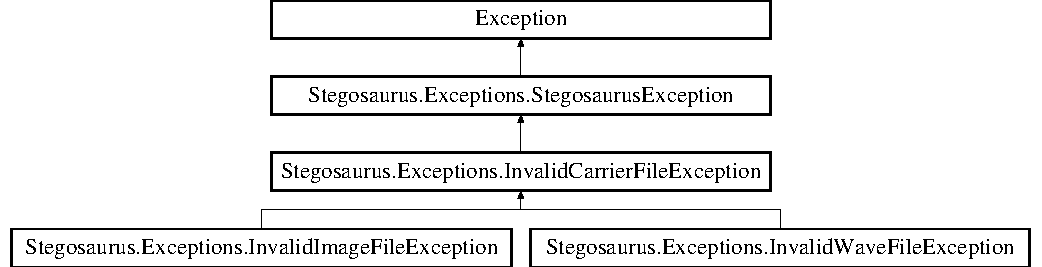
\includegraphics[height=3.578275cm]{class_stegosaurus_1_1_exceptions_1_1_invalid_carrier_file_exception}
\end{center}
\end{figure}
\subsection*{Public Member Functions}
\begin{DoxyCompactItemize}
\item 
{\bfseries Invalid\+Carrier\+File\+Exception} (string \+\_\+message, string \+\_\+file\+Name)\hypertarget{class_stegosaurus_1_1_exceptions_1_1_invalid_carrier_file_exception_a5b68424e30550e6bbec300316d10e205}{}\label{class_stegosaurus_1_1_exceptions_1_1_invalid_carrier_file_exception_a5b68424e30550e6bbec300316d10e205}

\end{DoxyCompactItemize}
\subsection*{Properties}
\begin{DoxyCompactItemize}
\item 
string {\bfseries File\+Name}\hspace{0.3cm}{\ttfamily  \mbox{[}get\mbox{]}}\hypertarget{class_stegosaurus_1_1_exceptions_1_1_invalid_carrier_file_exception_a029be7e676ff429dc4f51163d9f75d2c}{}\label{class_stegosaurus_1_1_exceptions_1_1_invalid_carrier_file_exception_a029be7e676ff429dc4f51163d9f75d2c}

\end{DoxyCompactItemize}


The documentation for this class was generated from the following file\+:\begin{DoxyCompactItemize}
\item 
Steganography/\+Stegosaurus/\+Exceptions/Invalid\+Carrier\+File\+Exception.\+cs\end{DoxyCompactItemize}

\hypertarget{class_stegosaurus_1_1_exceptions_1_1_invalid_image_file_exception}{}\section{Stegosaurus.\+Exceptions.\+Invalid\+Image\+File\+Exception Class Reference}
\label{class_stegosaurus_1_1_exceptions_1_1_invalid_image_file_exception}\index{Stegosaurus.\+Exceptions.\+Invalid\+Image\+File\+Exception@{Stegosaurus.\+Exceptions.\+Invalid\+Image\+File\+Exception}}
Inheritance diagram for Stegosaurus.\+Exceptions.\+Invalid\+Image\+File\+Exception\+:\begin{figure}[H]
\begin{center}
\leavevmode
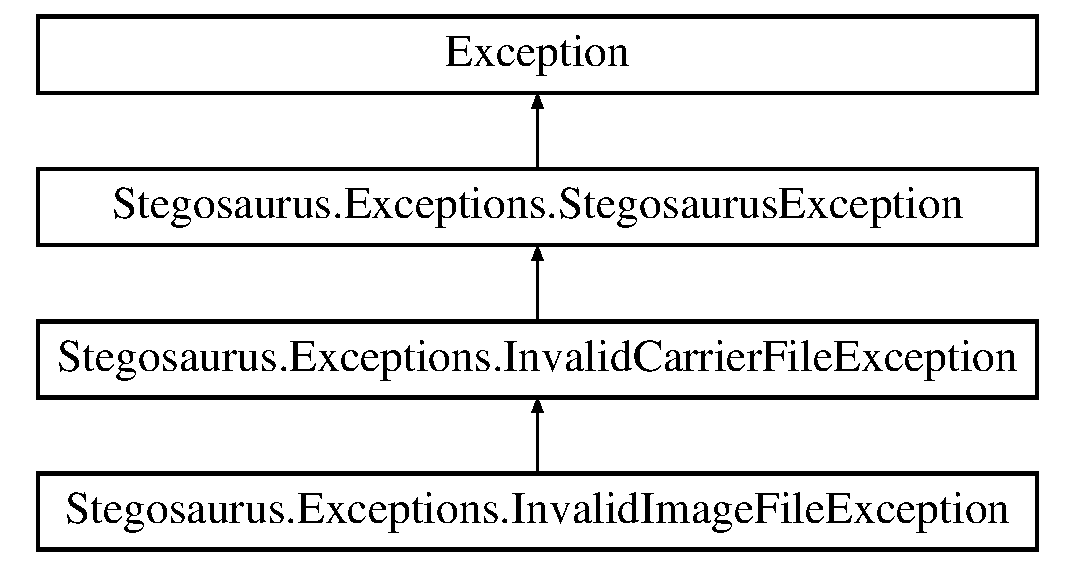
\includegraphics[height=4.000000cm]{class_stegosaurus_1_1_exceptions_1_1_invalid_image_file_exception}
\end{center}
\end{figure}
\subsection*{Public Member Functions}
\begin{DoxyCompactItemize}
\item 
{\bfseries Invalid\+Image\+File\+Exception} (string \+\_\+message, string \+\_\+file\+Name)\hypertarget{class_stegosaurus_1_1_exceptions_1_1_invalid_image_file_exception_ac833fccf38eca8e754118508b8b6b635}{}\label{class_stegosaurus_1_1_exceptions_1_1_invalid_image_file_exception_ac833fccf38eca8e754118508b8b6b635}

\end{DoxyCompactItemize}
\subsection*{Additional Inherited Members}


The documentation for this class was generated from the following file\+:\begin{DoxyCompactItemize}
\item 
Steganography/\+Stegosaurus/\+Exceptions/Invalid\+Image\+File\+Exception.\+cs\end{DoxyCompactItemize}

\hypertarget{class_stegosaurus_1_1_exceptions_1_1_invalid_wave_file_exception}{}\section{Stegosaurus.\+Exceptions.\+Invalid\+Wave\+File\+Exception Class Reference}
\label{class_stegosaurus_1_1_exceptions_1_1_invalid_wave_file_exception}\index{Stegosaurus.\+Exceptions.\+Invalid\+Wave\+File\+Exception@{Stegosaurus.\+Exceptions.\+Invalid\+Wave\+File\+Exception}}
Inheritance diagram for Stegosaurus.\+Exceptions.\+Invalid\+Wave\+File\+Exception\+:\begin{figure}[H]
\begin{center}
\leavevmode
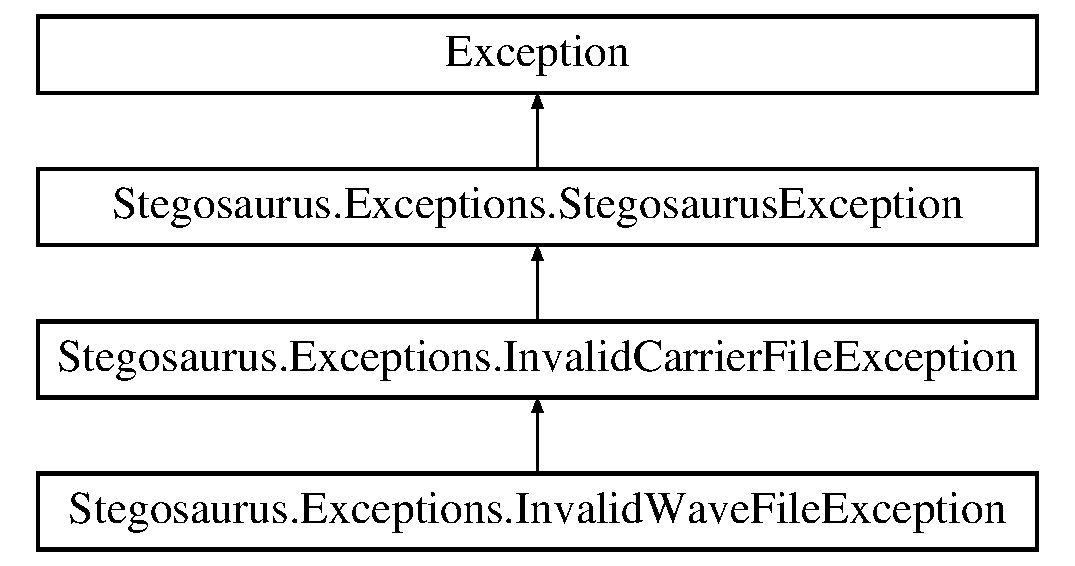
\includegraphics[height=4.000000cm]{class_stegosaurus_1_1_exceptions_1_1_invalid_wave_file_exception}
\end{center}
\end{figure}
\subsection*{Public Member Functions}
\begin{DoxyCompactItemize}
\item 
{\bfseries Invalid\+Wave\+File\+Exception} (string \+\_\+message, string \+\_\+file\+Name)\hypertarget{class_stegosaurus_1_1_exceptions_1_1_invalid_wave_file_exception_a845814b58b45eba6c3b7fcb7da160fd5}{}\label{class_stegosaurus_1_1_exceptions_1_1_invalid_wave_file_exception_a845814b58b45eba6c3b7fcb7da160fd5}

\end{DoxyCompactItemize}
\subsection*{Additional Inherited Members}


The documentation for this class was generated from the following file\+:\begin{DoxyCompactItemize}
\item 
Steganography/\+Stegosaurus/\+Exceptions/Invalid\+Wave\+File\+Exception.\+cs\end{DoxyCompactItemize}

\hypertarget{class_stegosaurus_1_1_algorithm_1_1_l_s_b_algorithm}{}\section{Stegosaurus.\+Algorithm.\+L\+S\+B\+Algorithm Class Reference}
\label{class_stegosaurus_1_1_algorithm_1_1_l_s_b_algorithm}\index{Stegosaurus.\+Algorithm.\+L\+S\+B\+Algorithm@{Stegosaurus.\+Algorithm.\+L\+S\+B\+Algorithm}}
Inheritance diagram for Stegosaurus.\+Algorithm.\+L\+S\+B\+Algorithm\+:\begin{figure}[H]
\begin{center}
\leavevmode
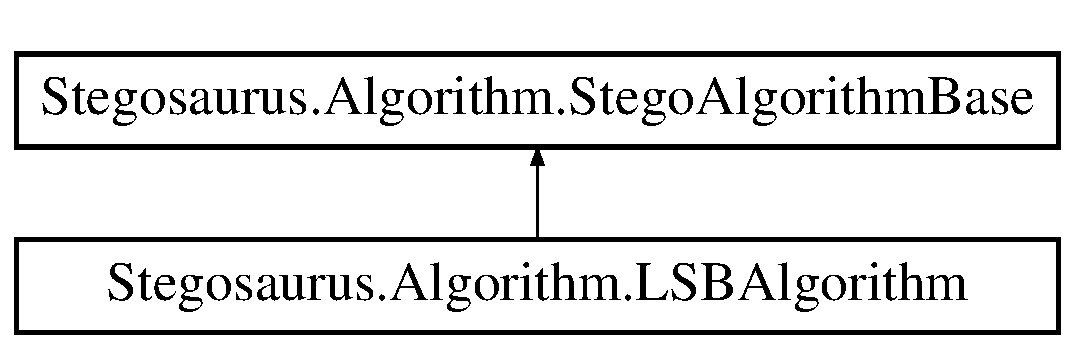
\includegraphics[height=2.000000cm]{class_stegosaurus_1_1_algorithm_1_1_l_s_b_algorithm}
\end{center}
\end{figure}
\subsection*{Public Types}
\begin{DoxyCompactItemize}
\item 
enum \hyperlink{class_stegosaurus_1_1_algorithm_1_1_l_s_b_algorithm_a8c5aef64ddbc41d8aeab953254b3c244}{Bit\+Values} \+: byte \{ \\*
{\bfseries First} = 0x1, 
{\bfseries Second} = 0x2, 
{\bfseries Third} = 0x4, 
{\bfseries Fourth} = 0x8, 
\\*
{\bfseries Fifth} = 0x10, 
{\bfseries Sixth} = 0x20, 
{\bfseries Seventh} = 0x40, 
{\bfseries Eighth} = 0x80
 \}\begin{DoxyCompactList}\small\item\em Enum containing the different bit values. \end{DoxyCompactList}
\end{DoxyCompactItemize}
\subsection*{Public Member Functions}
\begin{DoxyCompactItemize}
\item 
override void \hyperlink{class_stegosaurus_1_1_algorithm_1_1_l_s_b_algorithm_a8899e46584f804ea4c08741d6cc48b08}{Embed} (\hyperlink{class_stegosaurus_1_1_stego_message}{Stego\+Message} \+\_\+message, I\+Progress$<$ int $>$ \+\_\+progress, Cancellation\+Token \+\_\+ct)
\begin{DoxyCompactList}\small\item\em Embeds a \hyperlink{class_stegosaurus_1_1_stego_message}{Stego\+Message} in the public Byte\+Array of the Carrier\+Media. \end{DoxyCompactList}\item 
override \hyperlink{class_stegosaurus_1_1_stego_message}{Stego\+Message} \hyperlink{class_stegosaurus_1_1_algorithm_1_1_l_s_b_algorithm_a4c0597f5f93e47dc5a8ad58d06c9b189}{Extract} ()
\begin{DoxyCompactList}\small\item\em Returns a \hyperlink{class_stegosaurus_1_1_stego_message}{Stego\+Message} by extracting from the public Byte\+Array of the Carrier\+Media. \end{DoxyCompactList}\item 
override long \hyperlink{class_stegosaurus_1_1_algorithm_1_1_l_s_b_algorithm_a4e3b04a0820a9d819c38d5ec38d3eeaa}{Compute\+Bandwidth} ()
\begin{DoxyCompactList}\small\item\em Returns the data capacity of the carrier media with the given algorithm. \end{DoxyCompactList}\end{DoxyCompactItemize}
\subsection*{Public Attributes}
\begin{DoxyCompactItemize}
\item 
override string {\bfseries Name} =$>$ \char`\"{}Least Significant Bit\char`\"{}\hypertarget{class_stegosaurus_1_1_algorithm_1_1_l_s_b_algorithm_a4919f3b865726ed1c81a20214eb3bb4b}{}\label{class_stegosaurus_1_1_algorithm_1_1_l_s_b_algorithm_a4919f3b865726ed1c81a20214eb3bb4b}

\end{DoxyCompactItemize}
\subsection*{Protected Attributes}
\begin{DoxyCompactItemize}
\item 
override byte\mbox{[}$\,$\mbox{]} {\bfseries Signature} =$>$ new byte\mbox{[}$\,$\mbox{]} \{ 0x6\+C, 0x73, 0x62, 0x51 \}\hypertarget{class_stegosaurus_1_1_algorithm_1_1_l_s_b_algorithm_aaed083366d8d7791df589878cb5a80b4}{}\label{class_stegosaurus_1_1_algorithm_1_1_l_s_b_algorithm_aaed083366d8d7791df589878cb5a80b4}

\end{DoxyCompactItemize}
\subsection*{Properties}
\begin{DoxyCompactItemize}
\item 
\hyperlink{class_stegosaurus_1_1_algorithm_1_1_l_s_b_algorithm_a8c5aef64ddbc41d8aeab953254b3c244}{Bit\+Values} \hyperlink{class_stegosaurus_1_1_algorithm_1_1_l_s_b_algorithm_aa472d9a95ff87d372406e666707cac12}{Working\+Bit}\hspace{0.3cm}{\ttfamily  \mbox{[}get, set\mbox{]}}
\begin{DoxyCompactList}\small\item\em Get or set the bit that will be modified or read from. \end{DoxyCompactList}\end{DoxyCompactItemize}


\subsection{Member Enumeration Documentation}
\index{Stegosaurus\+::\+Algorithm\+::\+L\+S\+B\+Algorithm@{Stegosaurus\+::\+Algorithm\+::\+L\+S\+B\+Algorithm}!Bit\+Values@{Bit\+Values}}
\index{Bit\+Values@{Bit\+Values}!Stegosaurus\+::\+Algorithm\+::\+L\+S\+B\+Algorithm@{Stegosaurus\+::\+Algorithm\+::\+L\+S\+B\+Algorithm}}
\subsubsection[{\texorpdfstring{Bit\+Values}{BitValues}}]{\setlength{\rightskip}{0pt plus 5cm}enum {\bf Stegosaurus.\+Algorithm.\+L\+S\+B\+Algorithm.\+Bit\+Values} \+: byte\hspace{0.3cm}{\ttfamily [strong]}}\hypertarget{class_stegosaurus_1_1_algorithm_1_1_l_s_b_algorithm_a8c5aef64ddbc41d8aeab953254b3c244}{}\label{class_stegosaurus_1_1_algorithm_1_1_l_s_b_algorithm_a8c5aef64ddbc41d8aeab953254b3c244}


Enum containing the different bit values. 



\subsection{Member Function Documentation}
\index{Stegosaurus\+::\+Algorithm\+::\+L\+S\+B\+Algorithm@{Stegosaurus\+::\+Algorithm\+::\+L\+S\+B\+Algorithm}!Compute\+Bandwidth@{Compute\+Bandwidth}}
\index{Compute\+Bandwidth@{Compute\+Bandwidth}!Stegosaurus\+::\+Algorithm\+::\+L\+S\+B\+Algorithm@{Stegosaurus\+::\+Algorithm\+::\+L\+S\+B\+Algorithm}}
\subsubsection[{\texorpdfstring{Compute\+Bandwidth()}{ComputeBandwidth()}}]{\setlength{\rightskip}{0pt plus 5cm}override long Stegosaurus.\+Algorithm.\+L\+S\+B\+Algorithm.\+Compute\+Bandwidth (
\begin{DoxyParamCaption}
{}
\end{DoxyParamCaption}
)\hspace{0.3cm}{\ttfamily [virtual]}}\hypertarget{class_stegosaurus_1_1_algorithm_1_1_l_s_b_algorithm_a4e3b04a0820a9d819c38d5ec38d3eeaa}{}\label{class_stegosaurus_1_1_algorithm_1_1_l_s_b_algorithm_a4e3b04a0820a9d819c38d5ec38d3eeaa}


Returns the data capacity of the carrier media with the given algorithm. 



Implements \hyperlink{class_stegosaurus_1_1_algorithm_1_1_stego_algorithm_base_a2b4d2a0c3b65c980b5cbda2ab7601535}{Stegosaurus.\+Algorithm.\+Stego\+Algorithm\+Base}.

\index{Stegosaurus\+::\+Algorithm\+::\+L\+S\+B\+Algorithm@{Stegosaurus\+::\+Algorithm\+::\+L\+S\+B\+Algorithm}!Embed@{Embed}}
\index{Embed@{Embed}!Stegosaurus\+::\+Algorithm\+::\+L\+S\+B\+Algorithm@{Stegosaurus\+::\+Algorithm\+::\+L\+S\+B\+Algorithm}}
\subsubsection[{\texorpdfstring{Embed(\+Stego\+Message \+\_\+message, I\+Progress$<$ int $>$ \+\_\+progress, Cancellation\+Token \+\_\+ct)}{Embed(StegoMessage _message, IProgress< int > _progress, CancellationToken _ct)}}]{\setlength{\rightskip}{0pt plus 5cm}override void Stegosaurus.\+Algorithm.\+L\+S\+B\+Algorithm.\+Embed (
\begin{DoxyParamCaption}
\item[{{\bf Stego\+Message}}]{\+\_\+message, }
\item[{I\+Progress$<$ int $>$}]{\+\_\+progress, }
\item[{Cancellation\+Token}]{\+\_\+ct}
\end{DoxyParamCaption}
)\hspace{0.3cm}{\ttfamily [virtual]}}\hypertarget{class_stegosaurus_1_1_algorithm_1_1_l_s_b_algorithm_a8899e46584f804ea4c08741d6cc48b08}{}\label{class_stegosaurus_1_1_algorithm_1_1_l_s_b_algorithm_a8899e46584f804ea4c08741d6cc48b08}


Embeds a \hyperlink{class_stegosaurus_1_1_stego_message}{Stego\+Message} in the public Byte\+Array of the Carrier\+Media. 



Implements \hyperlink{class_stegosaurus_1_1_algorithm_1_1_stego_algorithm_base_aa0d6b5f8f24d0ef5f9f2126b32cbad47}{Stegosaurus.\+Algorithm.\+Stego\+Algorithm\+Base}.

\index{Stegosaurus\+::\+Algorithm\+::\+L\+S\+B\+Algorithm@{Stegosaurus\+::\+Algorithm\+::\+L\+S\+B\+Algorithm}!Extract@{Extract}}
\index{Extract@{Extract}!Stegosaurus\+::\+Algorithm\+::\+L\+S\+B\+Algorithm@{Stegosaurus\+::\+Algorithm\+::\+L\+S\+B\+Algorithm}}
\subsubsection[{\texorpdfstring{Extract()}{Extract()}}]{\setlength{\rightskip}{0pt plus 5cm}override {\bf Stego\+Message} Stegosaurus.\+Algorithm.\+L\+S\+B\+Algorithm.\+Extract (
\begin{DoxyParamCaption}
{}
\end{DoxyParamCaption}
)\hspace{0.3cm}{\ttfamily [virtual]}}\hypertarget{class_stegosaurus_1_1_algorithm_1_1_l_s_b_algorithm_a4c0597f5f93e47dc5a8ad58d06c9b189}{}\label{class_stegosaurus_1_1_algorithm_1_1_l_s_b_algorithm_a4c0597f5f93e47dc5a8ad58d06c9b189}


Returns a \hyperlink{class_stegosaurus_1_1_stego_message}{Stego\+Message} by extracting from the public Byte\+Array of the Carrier\+Media. 



Implements \hyperlink{class_stegosaurus_1_1_algorithm_1_1_stego_algorithm_base_a069eef0b17aa0221d2c111925b8d735a}{Stegosaurus.\+Algorithm.\+Stego\+Algorithm\+Base}.



\subsection{Property Documentation}
\index{Stegosaurus\+::\+Algorithm\+::\+L\+S\+B\+Algorithm@{Stegosaurus\+::\+Algorithm\+::\+L\+S\+B\+Algorithm}!Working\+Bit@{Working\+Bit}}
\index{Working\+Bit@{Working\+Bit}!Stegosaurus\+::\+Algorithm\+::\+L\+S\+B\+Algorithm@{Stegosaurus\+::\+Algorithm\+::\+L\+S\+B\+Algorithm}}
\subsubsection[{\texorpdfstring{Working\+Bit}{WorkingBit}}]{\setlength{\rightskip}{0pt plus 5cm}{\bf Bit\+Values} Stegosaurus.\+Algorithm.\+L\+S\+B\+Algorithm.\+Working\+Bit\hspace{0.3cm}{\ttfamily [get]}, {\ttfamily [set]}}\hypertarget{class_stegosaurus_1_1_algorithm_1_1_l_s_b_algorithm_aa472d9a95ff87d372406e666707cac12}{}\label{class_stegosaurus_1_1_algorithm_1_1_l_s_b_algorithm_aa472d9a95ff87d372406e666707cac12}


Get or set the bit that will be modified or read from. 



The documentation for this class was generated from the following file\+:\begin{DoxyCompactItemize}
\item 
Steganography/\+Stegosaurus/\+Algorithm/L\+S\+B\+Algorithm.\+cs\end{DoxyCompactItemize}

\hypertarget{class_stegosaurus_1_1_utility_1_1_random_number_list}{}\section{Stegosaurus.\+Utility.\+Random\+Number\+List Class Reference}
\label{class_stegosaurus_1_1_utility_1_1_random_number_list}\index{Stegosaurus.\+Utility.\+Random\+Number\+List@{Stegosaurus.\+Utility.\+Random\+Number\+List}}
\subsection*{Public Member Functions}
\begin{DoxyCompactItemize}
\item 
\hyperlink{class_stegosaurus_1_1_utility_1_1_random_number_list_aecb1a902942855613d04254663b2e415}{Random\+Number\+List} (int \+\_\+seed, int \+\_\+max\+Value)
\begin{DoxyCompactList}\small\item\em Construct a \hyperlink{class_stegosaurus_1_1_utility_1_1_random_number_list}{Random\+Number\+List} with a seed and maximum value. \end{DoxyCompactList}\end{DoxyCompactItemize}
\subsection*{Properties}
\begin{DoxyCompactItemize}
\item 
int \hyperlink{class_stegosaurus_1_1_utility_1_1_random_number_list_ae0059e85d2b7c12ec6d08cc28e206d5a}{Next}\hspace{0.3cm}{\ttfamily  \mbox{[}get\mbox{]}}
\begin{DoxyCompactList}\small\item\em Get the next integer in the random number sequence. Throws a Random\+Numbers\+Out\+Of\+Range\+Exception if there are no numbers left to generate. \end{DoxyCompactList}\end{DoxyCompactItemize}


\subsection{Constructor \& Destructor Documentation}
\index{Stegosaurus\+::\+Utility\+::\+Random\+Number\+List@{Stegosaurus\+::\+Utility\+::\+Random\+Number\+List}!Random\+Number\+List@{Random\+Number\+List}}
\index{Random\+Number\+List@{Random\+Number\+List}!Stegosaurus\+::\+Utility\+::\+Random\+Number\+List@{Stegosaurus\+::\+Utility\+::\+Random\+Number\+List}}
\subsubsection[{\texorpdfstring{Random\+Number\+List(int \+\_\+seed, int \+\_\+max\+Value)}{RandomNumberList(int _seed, int _maxValue)}}]{\setlength{\rightskip}{0pt plus 5cm}Stegosaurus.\+Utility.\+Random\+Number\+List.\+Random\+Number\+List (
\begin{DoxyParamCaption}
\item[{int}]{\+\_\+seed, }
\item[{int}]{\+\_\+max\+Value}
\end{DoxyParamCaption}
)}\hypertarget{class_stegosaurus_1_1_utility_1_1_random_number_list_aecb1a902942855613d04254663b2e415}{}\label{class_stegosaurus_1_1_utility_1_1_random_number_list_aecb1a902942855613d04254663b2e415}


Construct a \hyperlink{class_stegosaurus_1_1_utility_1_1_random_number_list}{Random\+Number\+List} with a seed and maximum value. 



\subsection{Property Documentation}
\index{Stegosaurus\+::\+Utility\+::\+Random\+Number\+List@{Stegosaurus\+::\+Utility\+::\+Random\+Number\+List}!Next@{Next}}
\index{Next@{Next}!Stegosaurus\+::\+Utility\+::\+Random\+Number\+List@{Stegosaurus\+::\+Utility\+::\+Random\+Number\+List}}
\subsubsection[{\texorpdfstring{Next}{Next}}]{\setlength{\rightskip}{0pt plus 5cm}int Stegosaurus.\+Utility.\+Random\+Number\+List.\+Next\hspace{0.3cm}{\ttfamily [get]}}\hypertarget{class_stegosaurus_1_1_utility_1_1_random_number_list_ae0059e85d2b7c12ec6d08cc28e206d5a}{}\label{class_stegosaurus_1_1_utility_1_1_random_number_list_ae0059e85d2b7c12ec6d08cc28e206d5a}


Get the next integer in the random number sequence. Throws a Random\+Numbers\+Out\+Of\+Range\+Exception if there are no numbers left to generate. 



The documentation for this class was generated from the following file\+:\begin{DoxyCompactItemize}
\item 
Steganography/\+Stegosaurus/\+Utility/Random\+Number\+List.\+cs\end{DoxyCompactItemize}

\hypertarget{class_stegosaurus_1_1_exceptions_1_1_random_numbers_out_of_range_exception}{}\section{Stegosaurus.\+Exceptions.\+Random\+Numbers\+Out\+Of\+Range\+Exception Class Reference}
\label{class_stegosaurus_1_1_exceptions_1_1_random_numbers_out_of_range_exception}\index{Stegosaurus.\+Exceptions.\+Random\+Numbers\+Out\+Of\+Range\+Exception@{Stegosaurus.\+Exceptions.\+Random\+Numbers\+Out\+Of\+Range\+Exception}}
Inheritance diagram for Stegosaurus.\+Exceptions.\+Random\+Numbers\+Out\+Of\+Range\+Exception\+:\begin{figure}[H]
\begin{center}
\leavevmode
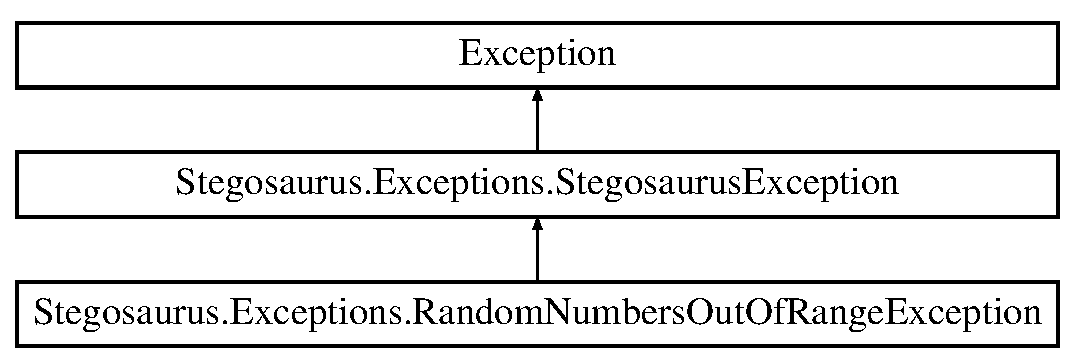
\includegraphics[height=3.000000cm]{class_stegosaurus_1_1_exceptions_1_1_random_numbers_out_of_range_exception}
\end{center}
\end{figure}
\subsection*{Additional Inherited Members}


The documentation for this class was generated from the following file\+:\begin{DoxyCompactItemize}
\item 
Steganography/\+Stegosaurus/\+Exceptions/Random\+Numbers\+Out\+Of\+Range\+Exception.\+cs\end{DoxyCompactItemize}

\hypertarget{class_stegosaurus_1_1_cryptography_1_1_r_s_a_key_pair}{}\section{Stegosaurus.\+Cryptography.\+R\+S\+A\+Key\+Pair Class Reference}
\label{class_stegosaurus_1_1_cryptography_1_1_r_s_a_key_pair}\index{Stegosaurus.\+Cryptography.\+R\+S\+A\+Key\+Pair@{Stegosaurus.\+Cryptography.\+R\+S\+A\+Key\+Pair}}
\subsection*{Properties}
\begin{DoxyCompactItemize}
\item 
string {\bfseries Public\+Key}\hspace{0.3cm}{\ttfamily  \mbox{[}get, set\mbox{]}}\hypertarget{class_stegosaurus_1_1_cryptography_1_1_r_s_a_key_pair_ac89d59ddb3d4df97c5a16df091f98be7}{}\label{class_stegosaurus_1_1_cryptography_1_1_r_s_a_key_pair_ac89d59ddb3d4df97c5a16df091f98be7}

\item 
string {\bfseries Private\+Key}\hspace{0.3cm}{\ttfamily  \mbox{[}get, set\mbox{]}}\hypertarget{class_stegosaurus_1_1_cryptography_1_1_r_s_a_key_pair_ae38147de52cb73bd84896c7ae9ca4746}{}\label{class_stegosaurus_1_1_cryptography_1_1_r_s_a_key_pair_ae38147de52cb73bd84896c7ae9ca4746}

\end{DoxyCompactItemize}


The documentation for this class was generated from the following file\+:\begin{DoxyCompactItemize}
\item 
Steganography/\+Stegosaurus/\+Cryptography/R\+S\+A\+Key\+Pair.\+cs\end{DoxyCompactItemize}

\hypertarget{class_stegosaurus_1_1_cryptography_1_1_r_s_a_provider}{}\section{Stegosaurus.\+Cryptography.\+R\+S\+A\+Provider Class Reference}
\label{class_stegosaurus_1_1_cryptography_1_1_r_s_a_provider}\index{Stegosaurus.\+Cryptography.\+R\+S\+A\+Provider@{Stegosaurus.\+Cryptography.\+R\+S\+A\+Provider}}
Inheritance diagram for Stegosaurus.\+Cryptography.\+R\+S\+A\+Provider\+:\begin{figure}[H]
\begin{center}
\leavevmode
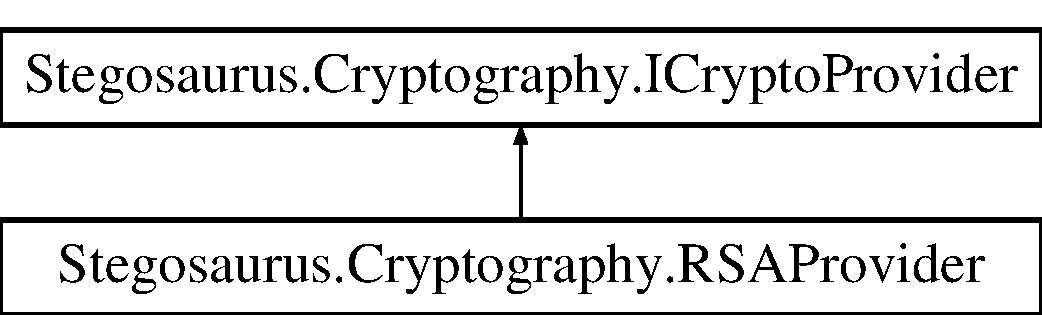
\includegraphics[height=2.000000cm]{class_stegosaurus_1_1_cryptography_1_1_r_s_a_provider}
\end{center}
\end{figure}
\subsection*{Public Member Functions}
\begin{DoxyCompactItemize}
\item 
byte\mbox{[}$\,$\mbox{]} \hyperlink{class_stegosaurus_1_1_cryptography_1_1_r_s_a_provider_ae5bf59d4baa636c5b3639cc24e240468}{Decrypt} (byte\mbox{[}$\,$\mbox{]} \+\_\+data)
\begin{DoxyCompactList}\small\item\em Decrypts and returns decrypted data. \end{DoxyCompactList}\item 
byte\mbox{[}$\,$\mbox{]} \hyperlink{class_stegosaurus_1_1_cryptography_1_1_r_s_a_provider_aa3b8f1d8c55043ca741b4ec3fd456836}{Encrypt} (byte\mbox{[}$\,$\mbox{]} \+\_\+data)
\begin{DoxyCompactList}\small\item\em Encrypts and returns encrypted data. \end{DoxyCompactList}\item 
void \hyperlink{class_stegosaurus_1_1_cryptography_1_1_r_s_a_provider_a18053ea1b1d9709c8631e97bef06c6a8}{Set\+Key} (string \+\_\+key\+String)
\begin{DoxyCompactList}\small\item\em Set the Key from a string. \end{DoxyCompactList}\item 
byte\mbox{[}$\,$\mbox{]} \hyperlink{class_stegosaurus_1_1_cryptography_1_1_r_s_a_provider_abf0779c0e2d3d295385af554c1776bc5}{Generate\+Key} ()
\begin{DoxyCompactList}\small\item\em Generates and returns a key which can be used with the algorithm. \end{DoxyCompactList}\end{DoxyCompactItemize}
\subsection*{Static Public Member Functions}
\begin{DoxyCompactItemize}
\item 
static \hyperlink{class_stegosaurus_1_1_cryptography_1_1_r_s_a_key_pair}{R\+S\+A\+Key\+Pair} {\bfseries Generate\+Keys} (int \+\_\+key\+Size)\hypertarget{class_stegosaurus_1_1_cryptography_1_1_r_s_a_provider_a23d4170a51bc7c17d8271a96c75b4e24}{}\label{class_stegosaurus_1_1_cryptography_1_1_r_s_a_provider_a23d4170a51bc7c17d8271a96c75b4e24}

\end{DoxyCompactItemize}
\subsection*{Public Attributes}
\begin{DoxyCompactItemize}
\item 
string {\bfseries Name} =$>$ \char`\"{}R\+SA\char`\"{}\hypertarget{class_stegosaurus_1_1_cryptography_1_1_r_s_a_provider_a68ff65d48e11ee45d1ef5bd48d6bfdb9}{}\label{class_stegosaurus_1_1_cryptography_1_1_r_s_a_provider_a68ff65d48e11ee45d1ef5bd48d6bfdb9}

\item 
int \hyperlink{class_stegosaurus_1_1_cryptography_1_1_r_s_a_provider_af73cf9dd65178ff5574b08072ea1a6c3}{Seed} =$>$ Key == null ? 0 \+: Parameters.\+Modulus.\+Compute\+Hash()
\begin{DoxyCompactList}\small\item\em The same seed is needed for encryption and decryption. Since the public and private key share modulus, we use its hash as a seed. \end{DoxyCompactList}\item 
int {\bfseries Key\+Size} =$>$ 2048\hypertarget{class_stegosaurus_1_1_cryptography_1_1_r_s_a_provider_a755fd6fc0a41a93c3a628df8e301b4ec}{}\label{class_stegosaurus_1_1_cryptography_1_1_r_s_a_provider_a755fd6fc0a41a93c3a628df8e301b4ec}

\end{DoxyCompactItemize}
\subsection*{Properties}
\begin{DoxyCompactItemize}
\item 
byte\mbox{[}$\,$\mbox{]} {\bfseries Key}\hspace{0.3cm}{\ttfamily  \mbox{[}get, set\mbox{]}}\hypertarget{class_stegosaurus_1_1_cryptography_1_1_r_s_a_provider_aa2493d643bf46387cc97a30c14da887f}{}\label{class_stegosaurus_1_1_cryptography_1_1_r_s_a_provider_aa2493d643bf46387cc97a30c14da887f}

\end{DoxyCompactItemize}


\subsection{Member Function Documentation}
\index{Stegosaurus\+::\+Cryptography\+::\+R\+S\+A\+Provider@{Stegosaurus\+::\+Cryptography\+::\+R\+S\+A\+Provider}!Decrypt@{Decrypt}}
\index{Decrypt@{Decrypt}!Stegosaurus\+::\+Cryptography\+::\+R\+S\+A\+Provider@{Stegosaurus\+::\+Cryptography\+::\+R\+S\+A\+Provider}}
\subsubsection[{\texorpdfstring{Decrypt(byte[] \+\_\+data)}{Decrypt(byte[] _data)}}]{\setlength{\rightskip}{0pt plus 5cm}byte \mbox{[}$\,$\mbox{]} Stegosaurus.\+Cryptography.\+R\+S\+A\+Provider.\+Decrypt (
\begin{DoxyParamCaption}
\item[{byte\mbox{[}$\,$\mbox{]}}]{\+\_\+data}
\end{DoxyParamCaption}
)}\hypertarget{class_stegosaurus_1_1_cryptography_1_1_r_s_a_provider_ae5bf59d4baa636c5b3639cc24e240468}{}\label{class_stegosaurus_1_1_cryptography_1_1_r_s_a_provider_ae5bf59d4baa636c5b3639cc24e240468}


Decrypts and returns decrypted data. 



Implements \hyperlink{interface_stegosaurus_1_1_cryptography_1_1_i_crypto_provider_a673607b0f3392591db9c647d2499f38d}{Stegosaurus.\+Cryptography.\+I\+Crypto\+Provider}.

\index{Stegosaurus\+::\+Cryptography\+::\+R\+S\+A\+Provider@{Stegosaurus\+::\+Cryptography\+::\+R\+S\+A\+Provider}!Encrypt@{Encrypt}}
\index{Encrypt@{Encrypt}!Stegosaurus\+::\+Cryptography\+::\+R\+S\+A\+Provider@{Stegosaurus\+::\+Cryptography\+::\+R\+S\+A\+Provider}}
\subsubsection[{\texorpdfstring{Encrypt(byte[] \+\_\+data)}{Encrypt(byte[] _data)}}]{\setlength{\rightskip}{0pt plus 5cm}byte \mbox{[}$\,$\mbox{]} Stegosaurus.\+Cryptography.\+R\+S\+A\+Provider.\+Encrypt (
\begin{DoxyParamCaption}
\item[{byte\mbox{[}$\,$\mbox{]}}]{\+\_\+data}
\end{DoxyParamCaption}
)}\hypertarget{class_stegosaurus_1_1_cryptography_1_1_r_s_a_provider_aa3b8f1d8c55043ca741b4ec3fd456836}{}\label{class_stegosaurus_1_1_cryptography_1_1_r_s_a_provider_aa3b8f1d8c55043ca741b4ec3fd456836}


Encrypts and returns encrypted data. 



Implements \hyperlink{interface_stegosaurus_1_1_cryptography_1_1_i_crypto_provider_a2222231bf16ba92e8efc8d515943aacd}{Stegosaurus.\+Cryptography.\+I\+Crypto\+Provider}.

\index{Stegosaurus\+::\+Cryptography\+::\+R\+S\+A\+Provider@{Stegosaurus\+::\+Cryptography\+::\+R\+S\+A\+Provider}!Generate\+Key@{Generate\+Key}}
\index{Generate\+Key@{Generate\+Key}!Stegosaurus\+::\+Cryptography\+::\+R\+S\+A\+Provider@{Stegosaurus\+::\+Cryptography\+::\+R\+S\+A\+Provider}}
\subsubsection[{\texorpdfstring{Generate\+Key()}{GenerateKey()}}]{\setlength{\rightskip}{0pt plus 5cm}byte \mbox{[}$\,$\mbox{]} Stegosaurus.\+Cryptography.\+R\+S\+A\+Provider.\+Generate\+Key (
\begin{DoxyParamCaption}
{}
\end{DoxyParamCaption}
)}\hypertarget{class_stegosaurus_1_1_cryptography_1_1_r_s_a_provider_abf0779c0e2d3d295385af554c1776bc5}{}\label{class_stegosaurus_1_1_cryptography_1_1_r_s_a_provider_abf0779c0e2d3d295385af554c1776bc5}


Generates and returns a key which can be used with the algorithm. 



Implements \hyperlink{interface_stegosaurus_1_1_cryptography_1_1_i_crypto_provider_ae25c64411409f0cc41c2282030c6dc5c}{Stegosaurus.\+Cryptography.\+I\+Crypto\+Provider}.

\index{Stegosaurus\+::\+Cryptography\+::\+R\+S\+A\+Provider@{Stegosaurus\+::\+Cryptography\+::\+R\+S\+A\+Provider}!Set\+Key@{Set\+Key}}
\index{Set\+Key@{Set\+Key}!Stegosaurus\+::\+Cryptography\+::\+R\+S\+A\+Provider@{Stegosaurus\+::\+Cryptography\+::\+R\+S\+A\+Provider}}
\subsubsection[{\texorpdfstring{Set\+Key(string \+\_\+key\+String)}{SetKey(string _keyString)}}]{\setlength{\rightskip}{0pt plus 5cm}void Stegosaurus.\+Cryptography.\+R\+S\+A\+Provider.\+Set\+Key (
\begin{DoxyParamCaption}
\item[{string}]{\+\_\+key\+String}
\end{DoxyParamCaption}
)}\hypertarget{class_stegosaurus_1_1_cryptography_1_1_r_s_a_provider_a18053ea1b1d9709c8631e97bef06c6a8}{}\label{class_stegosaurus_1_1_cryptography_1_1_r_s_a_provider_a18053ea1b1d9709c8631e97bef06c6a8}


Set the Key from a string. 



Implements \hyperlink{interface_stegosaurus_1_1_cryptography_1_1_i_crypto_provider_a95c1bb37e8bfdb62e6f66e8094d9d51b}{Stegosaurus.\+Cryptography.\+I\+Crypto\+Provider}.



\subsection{Member Data Documentation}
\index{Stegosaurus\+::\+Cryptography\+::\+R\+S\+A\+Provider@{Stegosaurus\+::\+Cryptography\+::\+R\+S\+A\+Provider}!Seed@{Seed}}
\index{Seed@{Seed}!Stegosaurus\+::\+Cryptography\+::\+R\+S\+A\+Provider@{Stegosaurus\+::\+Cryptography\+::\+R\+S\+A\+Provider}}
\subsubsection[{\texorpdfstring{Seed}{Seed}}]{\setlength{\rightskip}{0pt plus 5cm}int Stegosaurus.\+Cryptography.\+R\+S\+A\+Provider.\+Seed =$>$ Key == null ? 0 \+: Parameters.\+Modulus.\+Compute\+Hash()}\hypertarget{class_stegosaurus_1_1_cryptography_1_1_r_s_a_provider_af73cf9dd65178ff5574b08072ea1a6c3}{}\label{class_stegosaurus_1_1_cryptography_1_1_r_s_a_provider_af73cf9dd65178ff5574b08072ea1a6c3}


The same seed is needed for encryption and decryption. Since the public and private key share modulus, we use its hash as a seed. 



The documentation for this class was generated from the following file\+:\begin{DoxyCompactItemize}
\item 
Steganography/\+Stegosaurus/\+Cryptography/R\+S\+A\+Provider.\+cs\end{DoxyCompactItemize}

\hypertarget{class_stegosaurus_1_1_algorithm_1_1_graph_theory_1_1_sample}{}\section{Stegosaurus.\+Algorithm.\+Graph\+Theory.\+Sample Class Reference}
\label{class_stegosaurus_1_1_algorithm_1_1_graph_theory_1_1_sample}\index{Stegosaurus.\+Algorithm.\+Graph\+Theory.\+Sample@{Stegosaurus.\+Algorithm.\+Graph\+Theory.\+Sample}}
\subsection*{Public Member Functions}
\begin{DoxyCompactItemize}
\item 
{\bfseries Sample} (byte\mbox{[}$\,$\mbox{]} \+\_\+bytes)\hypertarget{class_stegosaurus_1_1_algorithm_1_1_graph_theory_1_1_sample_acf7995b54e7cc82441b14c9ed4d87335}{}\label{class_stegosaurus_1_1_algorithm_1_1_graph_theory_1_1_sample_acf7995b54e7cc82441b14c9ed4d87335}

\end{DoxyCompactItemize}
\subsection*{Public Attributes}
\begin{DoxyCompactItemize}
\item 
byte\mbox{[}$\,$\mbox{]} {\bfseries Bytes}\hypertarget{class_stegosaurus_1_1_algorithm_1_1_graph_theory_1_1_sample_aa7fb0e9e3eb6c2b8624b1185b2c730c7}{}\label{class_stegosaurus_1_1_algorithm_1_1_graph_theory_1_1_sample_aa7fb0e9e3eb6c2b8624b1185b2c730c7}

\item 
short {\bfseries Value}\hypertarget{class_stegosaurus_1_1_algorithm_1_1_graph_theory_1_1_sample_ae72ad88189265fae3073bd09a5b730fe}{}\label{class_stegosaurus_1_1_algorithm_1_1_graph_theory_1_1_sample_ae72ad88189265fae3073bd09a5b730fe}

\item 
short {\bfseries Target\+Value}\hypertarget{class_stegosaurus_1_1_algorithm_1_1_graph_theory_1_1_sample_a7d56edd7edef5ee7d2c1ef5197b45e83}{}\label{class_stegosaurus_1_1_algorithm_1_1_graph_theory_1_1_sample_a7d56edd7edef5ee7d2c1ef5197b45e83}

\end{DoxyCompactItemize}


The documentation for this class was generated from the following file\+:\begin{DoxyCompactItemize}
\item 
Steganography/\+Stegosaurus/\+Algorithm/\+Graph\+Theory/Sample.\+cs\end{DoxyCompactItemize}

\hypertarget{class_stegosaurus_1_1_algorithm_1_1_common_sample_1_1_sample}{}\section{Stegosaurus.\+Algorithm.\+Common\+Sample.\+Sample Class Reference}
\label{class_stegosaurus_1_1_algorithm_1_1_common_sample_1_1_sample}\index{Stegosaurus.\+Algorithm.\+Common\+Sample.\+Sample@{Stegosaurus.\+Algorithm.\+Common\+Sample.\+Sample}}
Inheritance diagram for Stegosaurus.\+Algorithm.\+Common\+Sample.\+Sample\+:\begin{figure}[H]
\begin{center}
\leavevmode
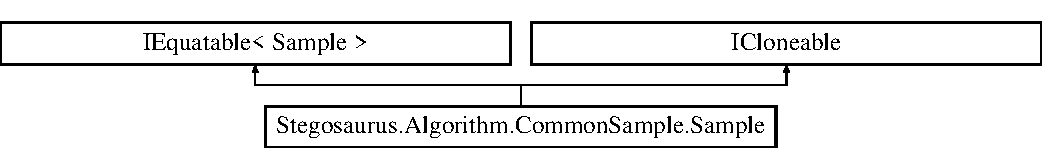
\includegraphics[height=1.964912cm]{class_stegosaurus_1_1_algorithm_1_1_common_sample_1_1_sample}
\end{center}
\end{figure}
\subsection*{Public Member Functions}
\begin{DoxyCompactItemize}
\item 
{\bfseries Sample} (params byte\mbox{[}$\,$\mbox{]} \+\_\+values)\hypertarget{class_stegosaurus_1_1_algorithm_1_1_common_sample_1_1_sample_ad688d64b22ce2864a4cc4d08da313066}{}\label{class_stegosaurus_1_1_algorithm_1_1_common_sample_1_1_sample_ad688d64b22ce2864a4cc4d08da313066}

\item 
void {\bfseries Force\+Changes} ()\hypertarget{class_stegosaurus_1_1_algorithm_1_1_common_sample_1_1_sample_adc55e15d2c2517c8768a7b356f434213}{}\label{class_stegosaurus_1_1_algorithm_1_1_common_sample_1_1_sample_adc55e15d2c2517c8768a7b356f434213}

\item 
void {\bfseries Update\+Mod\+Value} ()\hypertarget{class_stegosaurus_1_1_algorithm_1_1_common_sample_1_1_sample_ac24a03a70f19229ad7bbe06b9e5f616e}{}\label{class_stegosaurus_1_1_algorithm_1_1_common_sample_1_1_sample_ac24a03a70f19229ad7bbe06b9e5f616e}

\item 
int {\bfseries Distance\+To} (\hyperlink{class_stegosaurus_1_1_algorithm_1_1_common_sample_1_1_sample}{Sample} other\+Sample)\hypertarget{class_stegosaurus_1_1_algorithm_1_1_common_sample_1_1_sample_af7f8577432dc6b9f30a3be49a4c8d69d}{}\label{class_stegosaurus_1_1_algorithm_1_1_common_sample_1_1_sample_af7f8577432dc6b9f30a3be49a4c8d69d}

\item 
override int {\bfseries Get\+Hash\+Code} ()\hypertarget{class_stegosaurus_1_1_algorithm_1_1_common_sample_1_1_sample_a3bd248189fbbc5f07b39523207b41a71}{}\label{class_stegosaurus_1_1_algorithm_1_1_common_sample_1_1_sample_a3bd248189fbbc5f07b39523207b41a71}

\item 
bool {\bfseries Equals} (\hyperlink{class_stegosaurus_1_1_algorithm_1_1_common_sample_1_1_sample}{Sample} other)\hypertarget{class_stegosaurus_1_1_algorithm_1_1_common_sample_1_1_sample_a07c1134886a379bdff7cc6fb7070ea69}{}\label{class_stegosaurus_1_1_algorithm_1_1_common_sample_1_1_sample_a07c1134886a379bdff7cc6fb7070ea69}

\item 
object {\bfseries Clone} ()\hypertarget{class_stegosaurus_1_1_algorithm_1_1_common_sample_1_1_sample_a13da44f795443d04d214c0d6845ad137}{}\label{class_stegosaurus_1_1_algorithm_1_1_common_sample_1_1_sample_a13da44f795443d04d214c0d6845ad137}

\end{DoxyCompactItemize}
\subsection*{Static Public Member Functions}
\begin{DoxyCompactItemize}
\item 
static List$<$ \hyperlink{class_stegosaurus_1_1_algorithm_1_1_common_sample_1_1_sample}{Sample} $>$ \hyperlink{class_stegosaurus_1_1_algorithm_1_1_common_sample_1_1_sample_ae8e05cc119668551b2dc015a1970263f}{Get\+Sample\+List\+From} (\hyperlink{interface_stegosaurus_1_1_carrier_1_1_i_carrier_media}{I\+Carrier\+Media} \+\_\+carrier\+Media)
\begin{DoxyCompactList}\small\item\em Returns a list of all samples in the Carrier\+Media. \end{DoxyCompactList}\end{DoxyCompactItemize}
\subsection*{Properties}
\begin{DoxyCompactItemize}
\item 
byte\mbox{[}$\,$\mbox{]} {\bfseries Values}\hspace{0.3cm}{\ttfamily  \mbox{[}get, set\mbox{]}}\hypertarget{class_stegosaurus_1_1_algorithm_1_1_common_sample_1_1_sample_ab71c1b7401e42157082d56ee63e17418}{}\label{class_stegosaurus_1_1_algorithm_1_1_common_sample_1_1_sample_ab71c1b7401e42157082d56ee63e17418}

\item 
int {\bfseries Last\+Distance}\hspace{0.3cm}{\ttfamily  \mbox{[}get, set\mbox{]}}\hypertarget{class_stegosaurus_1_1_algorithm_1_1_common_sample_1_1_sample_abff4b45f44853f8b61e119c2275008be}{}\label{class_stegosaurus_1_1_algorithm_1_1_common_sample_1_1_sample_abff4b45f44853f8b61e119c2275008be}

\item 
int {\bfseries Mod\+Value}\hspace{0.3cm}{\ttfamily  \mbox{[}get, set\mbox{]}}\hypertarget{class_stegosaurus_1_1_algorithm_1_1_common_sample_1_1_sample_a385371615d5aa1cefd12648f7b4d4f1e}{}\label{class_stegosaurus_1_1_algorithm_1_1_common_sample_1_1_sample_a385371615d5aa1cefd12648f7b4d4f1e}

\end{DoxyCompactItemize}


\subsection{Member Function Documentation}
\index{Stegosaurus\+::\+Algorithm\+::\+Common\+Sample\+::\+Sample@{Stegosaurus\+::\+Algorithm\+::\+Common\+Sample\+::\+Sample}!Get\+Sample\+List\+From@{Get\+Sample\+List\+From}}
\index{Get\+Sample\+List\+From@{Get\+Sample\+List\+From}!Stegosaurus\+::\+Algorithm\+::\+Common\+Sample\+::\+Sample@{Stegosaurus\+::\+Algorithm\+::\+Common\+Sample\+::\+Sample}}
\subsubsection[{\texorpdfstring{Get\+Sample\+List\+From(\+I\+Carrier\+Media \+\_\+carrier\+Media)}{GetSampleListFrom(ICarrierMedia _carrierMedia)}}]{\setlength{\rightskip}{0pt plus 5cm}static List$<${\bf Sample}$>$ Stegosaurus.\+Algorithm.\+Common\+Sample.\+Sample.\+Get\+Sample\+List\+From (
\begin{DoxyParamCaption}
\item[{{\bf I\+Carrier\+Media}}]{\+\_\+carrier\+Media}
\end{DoxyParamCaption}
)\hspace{0.3cm}{\ttfamily [static]}}\hypertarget{class_stegosaurus_1_1_algorithm_1_1_common_sample_1_1_sample_ae8e05cc119668551b2dc015a1970263f}{}\label{class_stegosaurus_1_1_algorithm_1_1_common_sample_1_1_sample_ae8e05cc119668551b2dc015a1970263f}


Returns a list of all samples in the Carrier\+Media. 



The documentation for this class was generated from the following file\+:\begin{DoxyCompactItemize}
\item 
Steganography/\+Stegosaurus/\+Algorithm/\+Common\+Sample/Sample.\+cs\end{DoxyCompactItemize}

\hypertarget{class_stegosaurus_1_1_algorithm_1_1_stego_algorithm_base}{}\section{Stegosaurus.\+Algorithm.\+Stego\+Algorithm\+Base Class Reference}
\label{class_stegosaurus_1_1_algorithm_1_1_stego_algorithm_base}\index{Stegosaurus.\+Algorithm.\+Stego\+Algorithm\+Base@{Stegosaurus.\+Algorithm.\+Stego\+Algorithm\+Base}}
Inheritance diagram for Stegosaurus.\+Algorithm.\+Stego\+Algorithm\+Base\+:\begin{figure}[H]
\begin{center}
\leavevmode
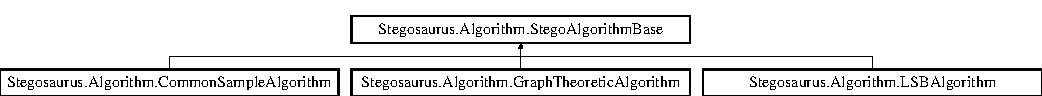
\includegraphics[height=1.274175cm]{class_stegosaurus_1_1_algorithm_1_1_stego_algorithm_base}
\end{center}
\end{figure}
\subsection*{Public Member Functions}
\begin{DoxyCompactItemize}
\item 
abstract long \hyperlink{class_stegosaurus_1_1_algorithm_1_1_stego_algorithm_base_a2b4d2a0c3b65c980b5cbda2ab7601535}{Compute\+Bandwidth} ()
\begin{DoxyCompactList}\small\item\em Returns the data capacity of the carrier media with the given algorithm. \end{DoxyCompactList}\item 
abstract void \hyperlink{class_stegosaurus_1_1_algorithm_1_1_stego_algorithm_base_aa0d6b5f8f24d0ef5f9f2126b32cbad47}{Embed} (\hyperlink{class_stegosaurus_1_1_stego_message}{Stego\+Message} \+\_\+message, I\+Progress$<$ int $>$ \+\_\+progress, Cancellation\+Token \+\_\+ct)
\begin{DoxyCompactList}\small\item\em Embeds a \hyperlink{class_stegosaurus_1_1_stego_message}{Stego\+Message} in the public Byte\+Array of the Carrier\+Media. \end{DoxyCompactList}\item 
abstract \hyperlink{class_stegosaurus_1_1_stego_message}{Stego\+Message} \hyperlink{class_stegosaurus_1_1_algorithm_1_1_stego_algorithm_base_a069eef0b17aa0221d2c111925b8d735a}{Extract} ()
\begin{DoxyCompactList}\small\item\em Returns a \hyperlink{class_stegosaurus_1_1_stego_message}{Stego\+Message} by extracting from the public Byte\+Array of the Carrier\+Media. \end{DoxyCompactList}\end{DoxyCompactItemize}
\subsection*{Protected Attributes}
\begin{DoxyCompactItemize}
\item 
virtual int \hyperlink{class_stegosaurus_1_1_algorithm_1_1_stego_algorithm_base_a8fb7f33711a582b1e102efa2c85e250f}{Seed} =$>$ \hyperlink{class_stegosaurus_1_1_algorithm_1_1_stego_algorithm_base_a58a15b795b59a77a818c12dd41b13841}{Crypto\+Provider}?.Seed ?? 0
\begin{DoxyCompactList}\small\item\em Get Seed used in pseudo-\/random pattern. \end{DoxyCompactList}\end{DoxyCompactItemize}
\subsection*{Properties}
\begin{DoxyCompactItemize}
\item 
abstract string \hyperlink{class_stegosaurus_1_1_algorithm_1_1_stego_algorithm_base_a348f32065aef0fec157f90d252edd71c}{Name}\hspace{0.3cm}{\ttfamily  \mbox{[}get\mbox{]}}
\begin{DoxyCompactList}\small\item\em Get the name of the algorithm. \end{DoxyCompactList}\item 
virtual \hyperlink{interface_stegosaurus_1_1_cryptography_1_1_i_crypto_provider}{I\+Crypto\+Provider} \hyperlink{class_stegosaurus_1_1_algorithm_1_1_stego_algorithm_base_a58a15b795b59a77a818c12dd41b13841}{Crypto\+Provider}\hspace{0.3cm}{\ttfamily  \mbox{[}get, set\mbox{]}}
\begin{DoxyCompactList}\small\item\em Get or set crypto provider. \end{DoxyCompactList}\item 
virtual \hyperlink{interface_stegosaurus_1_1_carrier_1_1_i_carrier_media}{I\+Carrier\+Media} \hyperlink{class_stegosaurus_1_1_algorithm_1_1_stego_algorithm_base_a5e77d196ee5a592ddf85184743c288e0}{Carrier\+Media}\hspace{0.3cm}{\ttfamily  \mbox{[}get, set\mbox{]}}
\begin{DoxyCompactList}\small\item\em Get or set Carrier\+Media. \end{DoxyCompactList}\item 
abstract byte\mbox{[}$\,$\mbox{]} \hyperlink{class_stegosaurus_1_1_algorithm_1_1_stego_algorithm_base_ace06936bcfcd9e9d9bb08ff97b1144f0}{Signature}\hspace{0.3cm}{\ttfamily  \mbox{[}get\mbox{]}}
\begin{DoxyCompactList}\small\item\em Get signature. \end{DoxyCompactList}\end{DoxyCompactItemize}


\subsection{Member Function Documentation}
\index{Stegosaurus\+::\+Algorithm\+::\+Stego\+Algorithm\+Base@{Stegosaurus\+::\+Algorithm\+::\+Stego\+Algorithm\+Base}!Compute\+Bandwidth@{Compute\+Bandwidth}}
\index{Compute\+Bandwidth@{Compute\+Bandwidth}!Stegosaurus\+::\+Algorithm\+::\+Stego\+Algorithm\+Base@{Stegosaurus\+::\+Algorithm\+::\+Stego\+Algorithm\+Base}}
\subsubsection[{\texorpdfstring{Compute\+Bandwidth()}{ComputeBandwidth()}}]{\setlength{\rightskip}{0pt plus 5cm}abstract long Stegosaurus.\+Algorithm.\+Stego\+Algorithm\+Base.\+Compute\+Bandwidth (
\begin{DoxyParamCaption}
{}
\end{DoxyParamCaption}
)\hspace{0.3cm}{\ttfamily [pure virtual]}}\hypertarget{class_stegosaurus_1_1_algorithm_1_1_stego_algorithm_base_a2b4d2a0c3b65c980b5cbda2ab7601535}{}\label{class_stegosaurus_1_1_algorithm_1_1_stego_algorithm_base_a2b4d2a0c3b65c980b5cbda2ab7601535}


Returns the data capacity of the carrier media with the given algorithm. 



Implemented in \hyperlink{class_stegosaurus_1_1_algorithm_1_1_common_sample_algorithm_aeb094a2d87af7b06f7710b79915164d8}{Stegosaurus.\+Algorithm.\+Common\+Sample\+Algorithm}, \hyperlink{class_stegosaurus_1_1_algorithm_1_1_l_s_b_algorithm_a4e3b04a0820a9d819c38d5ec38d3eeaa}{Stegosaurus.\+Algorithm.\+L\+S\+B\+Algorithm}, and \hyperlink{class_stegosaurus_1_1_algorithm_1_1_graph_theoretic_algorithm_aa3c0280792593fa75af74a7e3b9e8acc}{Stegosaurus.\+Algorithm.\+Graph\+Theoretic\+Algorithm}.

\index{Stegosaurus\+::\+Algorithm\+::\+Stego\+Algorithm\+Base@{Stegosaurus\+::\+Algorithm\+::\+Stego\+Algorithm\+Base}!Embed@{Embed}}
\index{Embed@{Embed}!Stegosaurus\+::\+Algorithm\+::\+Stego\+Algorithm\+Base@{Stegosaurus\+::\+Algorithm\+::\+Stego\+Algorithm\+Base}}
\subsubsection[{\texorpdfstring{Embed(\+Stego\+Message \+\_\+message, I\+Progress$<$ int $>$ \+\_\+progress, Cancellation\+Token \+\_\+ct)}{Embed(StegoMessage _message, IProgress< int > _progress, CancellationToken _ct)}}]{\setlength{\rightskip}{0pt plus 5cm}abstract void Stegosaurus.\+Algorithm.\+Stego\+Algorithm\+Base.\+Embed (
\begin{DoxyParamCaption}
\item[{{\bf Stego\+Message}}]{\+\_\+message, }
\item[{I\+Progress$<$ int $>$}]{\+\_\+progress, }
\item[{Cancellation\+Token}]{\+\_\+ct}
\end{DoxyParamCaption}
)\hspace{0.3cm}{\ttfamily [pure virtual]}}\hypertarget{class_stegosaurus_1_1_algorithm_1_1_stego_algorithm_base_aa0d6b5f8f24d0ef5f9f2126b32cbad47}{}\label{class_stegosaurus_1_1_algorithm_1_1_stego_algorithm_base_aa0d6b5f8f24d0ef5f9f2126b32cbad47}


Embeds a \hyperlink{class_stegosaurus_1_1_stego_message}{Stego\+Message} in the public Byte\+Array of the Carrier\+Media. 



Implemented in \hyperlink{class_stegosaurus_1_1_algorithm_1_1_graph_theoretic_algorithm_aecdce8aef6a5723d66bc93ca6f959767}{Stegosaurus.\+Algorithm.\+Graph\+Theoretic\+Algorithm}, \hyperlink{class_stegosaurus_1_1_algorithm_1_1_l_s_b_algorithm_a8899e46584f804ea4c08741d6cc48b08}{Stegosaurus.\+Algorithm.\+L\+S\+B\+Algorithm}, and \hyperlink{class_stegosaurus_1_1_algorithm_1_1_common_sample_algorithm_ab25967eede4bbf5ea54d64b168e4ae73}{Stegosaurus.\+Algorithm.\+Common\+Sample\+Algorithm}.

\index{Stegosaurus\+::\+Algorithm\+::\+Stego\+Algorithm\+Base@{Stegosaurus\+::\+Algorithm\+::\+Stego\+Algorithm\+Base}!Extract@{Extract}}
\index{Extract@{Extract}!Stegosaurus\+::\+Algorithm\+::\+Stego\+Algorithm\+Base@{Stegosaurus\+::\+Algorithm\+::\+Stego\+Algorithm\+Base}}
\subsubsection[{\texorpdfstring{Extract()}{Extract()}}]{\setlength{\rightskip}{0pt plus 5cm}abstract {\bf Stego\+Message} Stegosaurus.\+Algorithm.\+Stego\+Algorithm\+Base.\+Extract (
\begin{DoxyParamCaption}
{}
\end{DoxyParamCaption}
)\hspace{0.3cm}{\ttfamily [pure virtual]}}\hypertarget{class_stegosaurus_1_1_algorithm_1_1_stego_algorithm_base_a069eef0b17aa0221d2c111925b8d735a}{}\label{class_stegosaurus_1_1_algorithm_1_1_stego_algorithm_base_a069eef0b17aa0221d2c111925b8d735a}


Returns a \hyperlink{class_stegosaurus_1_1_stego_message}{Stego\+Message} by extracting from the public Byte\+Array of the Carrier\+Media. 



Implemented in \hyperlink{class_stegosaurus_1_1_algorithm_1_1_graph_theoretic_algorithm_ae12e30f823e7cedc1f3ae75fa8a914fb}{Stegosaurus.\+Algorithm.\+Graph\+Theoretic\+Algorithm}, \hyperlink{class_stegosaurus_1_1_algorithm_1_1_common_sample_algorithm_aab6487375c07bb4e77c719bb96605ad4}{Stegosaurus.\+Algorithm.\+Common\+Sample\+Algorithm}, and \hyperlink{class_stegosaurus_1_1_algorithm_1_1_l_s_b_algorithm_a4c0597f5f93e47dc5a8ad58d06c9b189}{Stegosaurus.\+Algorithm.\+L\+S\+B\+Algorithm}.



\subsection{Member Data Documentation}
\index{Stegosaurus\+::\+Algorithm\+::\+Stego\+Algorithm\+Base@{Stegosaurus\+::\+Algorithm\+::\+Stego\+Algorithm\+Base}!Seed@{Seed}}
\index{Seed@{Seed}!Stegosaurus\+::\+Algorithm\+::\+Stego\+Algorithm\+Base@{Stegosaurus\+::\+Algorithm\+::\+Stego\+Algorithm\+Base}}
\subsubsection[{\texorpdfstring{Seed}{Seed}}]{\setlength{\rightskip}{0pt plus 5cm}virtual int Stegosaurus.\+Algorithm.\+Stego\+Algorithm\+Base.\+Seed =$>$ {\bf Crypto\+Provider}?.Seed ?? 0\hspace{0.3cm}{\ttfamily [protected]}}\hypertarget{class_stegosaurus_1_1_algorithm_1_1_stego_algorithm_base_a8fb7f33711a582b1e102efa2c85e250f}{}\label{class_stegosaurus_1_1_algorithm_1_1_stego_algorithm_base_a8fb7f33711a582b1e102efa2c85e250f}


Get Seed used in pseudo-\/random pattern. 



\subsection{Property Documentation}
\index{Stegosaurus\+::\+Algorithm\+::\+Stego\+Algorithm\+Base@{Stegosaurus\+::\+Algorithm\+::\+Stego\+Algorithm\+Base}!Carrier\+Media@{Carrier\+Media}}
\index{Carrier\+Media@{Carrier\+Media}!Stegosaurus\+::\+Algorithm\+::\+Stego\+Algorithm\+Base@{Stegosaurus\+::\+Algorithm\+::\+Stego\+Algorithm\+Base}}
\subsubsection[{\texorpdfstring{Carrier\+Media}{CarrierMedia}}]{\setlength{\rightskip}{0pt plus 5cm}virtual {\bf I\+Carrier\+Media} Stegosaurus.\+Algorithm.\+Stego\+Algorithm\+Base.\+Carrier\+Media\hspace{0.3cm}{\ttfamily [get]}, {\ttfamily [set]}}\hypertarget{class_stegosaurus_1_1_algorithm_1_1_stego_algorithm_base_a5e77d196ee5a592ddf85184743c288e0}{}\label{class_stegosaurus_1_1_algorithm_1_1_stego_algorithm_base_a5e77d196ee5a592ddf85184743c288e0}


Get or set Carrier\+Media. 

\index{Stegosaurus\+::\+Algorithm\+::\+Stego\+Algorithm\+Base@{Stegosaurus\+::\+Algorithm\+::\+Stego\+Algorithm\+Base}!Crypto\+Provider@{Crypto\+Provider}}
\index{Crypto\+Provider@{Crypto\+Provider}!Stegosaurus\+::\+Algorithm\+::\+Stego\+Algorithm\+Base@{Stegosaurus\+::\+Algorithm\+::\+Stego\+Algorithm\+Base}}
\subsubsection[{\texorpdfstring{Crypto\+Provider}{CryptoProvider}}]{\setlength{\rightskip}{0pt plus 5cm}virtual {\bf I\+Crypto\+Provider} Stegosaurus.\+Algorithm.\+Stego\+Algorithm\+Base.\+Crypto\+Provider\hspace{0.3cm}{\ttfamily [get]}, {\ttfamily [set]}}\hypertarget{class_stegosaurus_1_1_algorithm_1_1_stego_algorithm_base_a58a15b795b59a77a818c12dd41b13841}{}\label{class_stegosaurus_1_1_algorithm_1_1_stego_algorithm_base_a58a15b795b59a77a818c12dd41b13841}


Get or set crypto provider. 

\index{Stegosaurus\+::\+Algorithm\+::\+Stego\+Algorithm\+Base@{Stegosaurus\+::\+Algorithm\+::\+Stego\+Algorithm\+Base}!Name@{Name}}
\index{Name@{Name}!Stegosaurus\+::\+Algorithm\+::\+Stego\+Algorithm\+Base@{Stegosaurus\+::\+Algorithm\+::\+Stego\+Algorithm\+Base}}
\subsubsection[{\texorpdfstring{Name}{Name}}]{\setlength{\rightskip}{0pt plus 5cm}abstract string Stegosaurus.\+Algorithm.\+Stego\+Algorithm\+Base.\+Name\hspace{0.3cm}{\ttfamily [get]}}\hypertarget{class_stegosaurus_1_1_algorithm_1_1_stego_algorithm_base_a348f32065aef0fec157f90d252edd71c}{}\label{class_stegosaurus_1_1_algorithm_1_1_stego_algorithm_base_a348f32065aef0fec157f90d252edd71c}


Get the name of the algorithm. 

\index{Stegosaurus\+::\+Algorithm\+::\+Stego\+Algorithm\+Base@{Stegosaurus\+::\+Algorithm\+::\+Stego\+Algorithm\+Base}!Signature@{Signature}}
\index{Signature@{Signature}!Stegosaurus\+::\+Algorithm\+::\+Stego\+Algorithm\+Base@{Stegosaurus\+::\+Algorithm\+::\+Stego\+Algorithm\+Base}}
\subsubsection[{\texorpdfstring{Signature}{Signature}}]{\setlength{\rightskip}{0pt plus 5cm}abstract byte \mbox{[}$\,$\mbox{]} Stegosaurus.\+Algorithm.\+Stego\+Algorithm\+Base.\+Signature\hspace{0.3cm}{\ttfamily [get]}, {\ttfamily [protected]}}\hypertarget{class_stegosaurus_1_1_algorithm_1_1_stego_algorithm_base_ace06936bcfcd9e9d9bb08ff97b1144f0}{}\label{class_stegosaurus_1_1_algorithm_1_1_stego_algorithm_base_ace06936bcfcd9e9d9bb08ff97b1144f0}


Get signature. 



The documentation for this class was generated from the following file\+:\begin{DoxyCompactItemize}
\item 
Steganography/\+Stegosaurus/\+Algorithm/Stego\+Algorithm\+Base.\+cs\end{DoxyCompactItemize}

\hypertarget{class_stegosaurus_1_1_exceptions_1_1_stego_algorithm_exception}{}\section{Stegosaurus.\+Exceptions.\+Stego\+Algorithm\+Exception Class Reference}
\label{class_stegosaurus_1_1_exceptions_1_1_stego_algorithm_exception}\index{Stegosaurus.\+Exceptions.\+Stego\+Algorithm\+Exception@{Stegosaurus.\+Exceptions.\+Stego\+Algorithm\+Exception}}
Inheritance diagram for Stegosaurus.\+Exceptions.\+Stego\+Algorithm\+Exception\+:\begin{figure}[H]
\begin{center}
\leavevmode
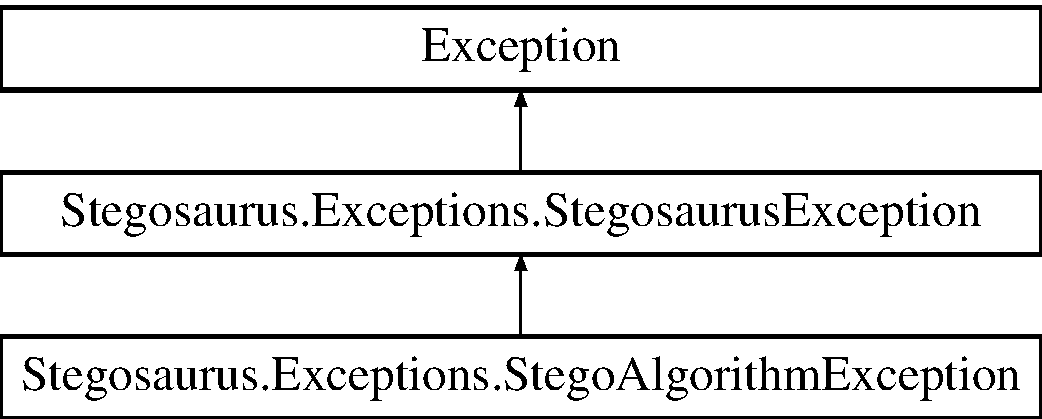
\includegraphics[height=3.000000cm]{class_stegosaurus_1_1_exceptions_1_1_stego_algorithm_exception}
\end{center}
\end{figure}
\subsection*{Public Member Functions}
\begin{DoxyCompactItemize}
\item 
{\bfseries Stego\+Algorithm\+Exception} (string message)\hypertarget{class_stegosaurus_1_1_exceptions_1_1_stego_algorithm_exception_afc9700030f15037383e5d4e946e6e5bf}{}\label{class_stegosaurus_1_1_exceptions_1_1_stego_algorithm_exception_afc9700030f15037383e5d4e946e6e5bf}

\end{DoxyCompactItemize}


The documentation for this class was generated from the following file\+:\begin{DoxyCompactItemize}
\item 
Steganography/\+Stegosaurus/\+Exceptions/Stego\+Algorithm\+Exception.\+cs\end{DoxyCompactItemize}

\hypertarget{class_stegosaurus_1_1_exceptions_1_1_stego_crypto_exception}{}\section{Stegosaurus.\+Exceptions.\+Stego\+Crypto\+Exception Class Reference}
\label{class_stegosaurus_1_1_exceptions_1_1_stego_crypto_exception}\index{Stegosaurus.\+Exceptions.\+Stego\+Crypto\+Exception@{Stegosaurus.\+Exceptions.\+Stego\+Crypto\+Exception}}
Inheritance diagram for Stegosaurus.\+Exceptions.\+Stego\+Crypto\+Exception\+:\begin{figure}[H]
\begin{center}
\leavevmode
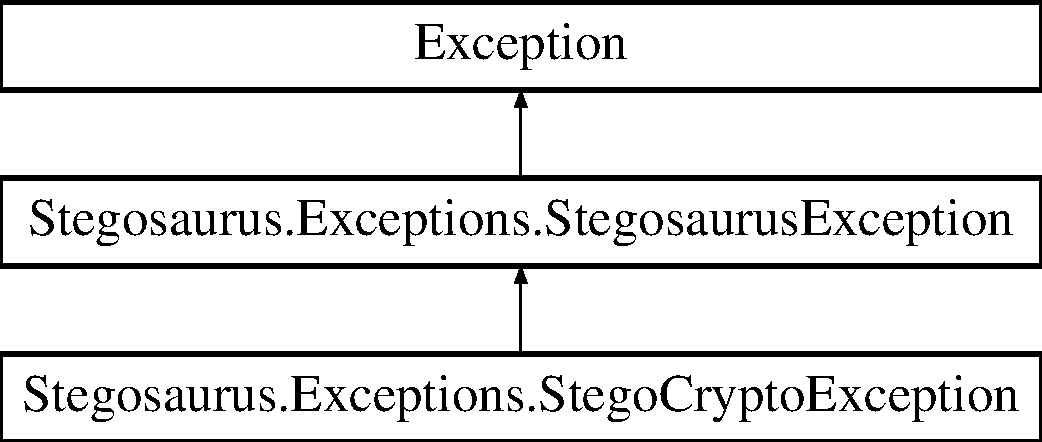
\includegraphics[height=3.000000cm]{class_stegosaurus_1_1_exceptions_1_1_stego_crypto_exception}
\end{center}
\end{figure}
\subsection*{Public Member Functions}
\begin{DoxyCompactItemize}
\item 
{\bfseries Stego\+Crypto\+Exception} (string message)\hypertarget{class_stegosaurus_1_1_exceptions_1_1_stego_crypto_exception_a87c4de3568884c827b238f8afaa50646}{}\label{class_stegosaurus_1_1_exceptions_1_1_stego_crypto_exception_a87c4de3568884c827b238f8afaa50646}

\item 
{\bfseries Stego\+Crypto\+Exception} (string message, Exception inner)\hypertarget{class_stegosaurus_1_1_exceptions_1_1_stego_crypto_exception_ad2e4e6e887d4c64801eb9465f7c4129a}{}\label{class_stegosaurus_1_1_exceptions_1_1_stego_crypto_exception_ad2e4e6e887d4c64801eb9465f7c4129a}

\end{DoxyCompactItemize}


The documentation for this class was generated from the following file\+:\begin{DoxyCompactItemize}
\item 
Steganography/\+Stegosaurus/\+Exceptions/Stego\+Crypto\+Exception.\+cs\end{DoxyCompactItemize}

\hypertarget{class_stegosaurus_1_1_stego_message}{}\section{Stegosaurus.\+Stego\+Message Class Reference}
\label{class_stegosaurus_1_1_stego_message}\index{Stegosaurus.\+Stego\+Message@{Stegosaurus.\+Stego\+Message}}
\subsection*{Public Types}
\begin{DoxyCompactItemize}
\item 
enum {\bfseries Stego\+Message\+Flags} \{ {\bfseries Encoded} = 0x1, 
{\bfseries Compressed} = 0x2, 
{\bfseries Encrypted} = 0x4, 
{\bfseries Signed} = 0x8
 \}\hypertarget{class_stegosaurus_1_1_stego_message_aae629068f4db90b3298479ee27c7f6a4}{}\label{class_stegosaurus_1_1_stego_message_aae629068f4db90b3298479ee27c7f6a4}

\end{DoxyCompactItemize}
\subsection*{Public Member Functions}
\begin{DoxyCompactItemize}
\item 
\hyperlink{class_stegosaurus_1_1_stego_message_a0c77527382a7b96dcee471eeb6c6d33b}{Stego\+Message} ()
\begin{DoxyCompactList}\small\item\em Empty constructor. \end{DoxyCompactList}\item 
\hyperlink{class_stegosaurus_1_1_stego_message_ab51641b56506698542fd1c1b6aed778e}{Stego\+Message} (string \+\_\+text\+Message)
\begin{DoxyCompactList}\small\item\em This constructer is used if only a text message is applied. \end{DoxyCompactList}\item 
\hyperlink{class_stegosaurus_1_1_stego_message_ae860989f48b4c55af65481fa292fb9b4}{Stego\+Message} (byte\mbox{[}$\,$\mbox{]} \+\_\+from\+Array, \hyperlink{interface_stegosaurus_1_1_cryptography_1_1_i_crypto_provider}{I\+Crypto\+Provider} \+\_\+crypto\+Provider=null)
\begin{DoxyCompactList}\small\item\em This constructer takes a byte array containing the data to add to the \hyperlink{class_stegosaurus_1_1_stego_message}{Stego\+Message}. \end{DoxyCompactList}\item 
byte\mbox{[}$\,$\mbox{]} \hyperlink{class_stegosaurus_1_1_stego_message_abf4c305d1dddbfd3b769d7bbc35bfcf3}{To\+Byte\+Array} (\hyperlink{interface_stegosaurus_1_1_cryptography_1_1_i_crypto_provider}{I\+Crypto\+Provider} \+\_\+crypto\+Provider=null)
\begin{DoxyCompactList}\small\item\em Converts text and/or file(s) into a byte array and combines them using a List. First part of the byte array contains the message file(s). The last part of the byte array is the text message if there is any. \end{DoxyCompactList}\item 
long \hyperlink{class_stegosaurus_1_1_stego_message_a3333bd46cd0c2f04f9a9352c52cfd95d}{Get\+Compressed\+Size} ()
\begin{DoxyCompactList}\small\item\em This method returns the compressed size of the data stored in this \hyperlink{class_stegosaurus_1_1_stego_message}{Stego\+Message}. \end{DoxyCompactList}\end{DoxyCompactItemize}
\subsection*{Public Attributes}
\begin{DoxyCompactItemize}
\item 
Stego\+Message\+Flags {\bfseries Flags} = new List$<$\hyperlink{class_stegosaurus_1_1_input_file}{Input\+File}$>$()\hypertarget{class_stegosaurus_1_1_stego_message_a1ec3adc5e452b5c512b1c0ee3c86e6d8}{}\label{class_stegosaurus_1_1_stego_message_a1ec3adc5e452b5c512b1c0ee3c86e6d8}

\end{DoxyCompactItemize}
\subsection*{Properties}
\begin{DoxyCompactItemize}
\item 
string \hyperlink{class_stegosaurus_1_1_stego_message_ab37f4ee21d0891f86693576a7d2bd389}{Text\+Message}\hspace{0.3cm}{\ttfamily  \mbox{[}get, set\mbox{]}}
\begin{DoxyCompactList}\small\item\em This is the text message that can be saved in the \hyperlink{class_stegosaurus_1_1_stego_message}{Stego\+Message}. \end{DoxyCompactList}\item 
List$<$ \hyperlink{class_stegosaurus_1_1_input_file}{Input\+File} $>$ \hyperlink{class_stegosaurus_1_1_stego_message_a284ab72c2bb641cabe1a09de8d46de6a}{Input\+Files}\hspace{0.3cm}{\ttfamily  \mbox{[}get\mbox{]}}
\begin{DoxyCompactList}\small\item\em This is where each file will be stored in the \hyperlink{class_stegosaurus_1_1_stego_message}{Stego\+Message}. \end{DoxyCompactList}\item 
string \hyperlink{class_stegosaurus_1_1_stego_message_a8fa8e3dce966a2fa578d74267f8d2a15}{Private\+Signing\+Key}\hspace{0.3cm}{\ttfamily  \mbox{[}get, set\mbox{]}}
\begin{DoxyCompactList}\small\item\em T\+O\+DO\+: Write summary. \end{DoxyCompactList}\end{DoxyCompactItemize}


\subsection{Constructor \& Destructor Documentation}
\index{Stegosaurus\+::\+Stego\+Message@{Stegosaurus\+::\+Stego\+Message}!Stego\+Message@{Stego\+Message}}
\index{Stego\+Message@{Stego\+Message}!Stegosaurus\+::\+Stego\+Message@{Stegosaurus\+::\+Stego\+Message}}
\subsubsection[{\texorpdfstring{Stego\+Message()}{StegoMessage()}}]{\setlength{\rightskip}{0pt plus 5cm}Stegosaurus.\+Stego\+Message.\+Stego\+Message (
\begin{DoxyParamCaption}
{}
\end{DoxyParamCaption}
)}\hypertarget{class_stegosaurus_1_1_stego_message_a0c77527382a7b96dcee471eeb6c6d33b}{}\label{class_stegosaurus_1_1_stego_message_a0c77527382a7b96dcee471eeb6c6d33b}


Empty constructor. 

\index{Stegosaurus\+::\+Stego\+Message@{Stegosaurus\+::\+Stego\+Message}!Stego\+Message@{Stego\+Message}}
\index{Stego\+Message@{Stego\+Message}!Stegosaurus\+::\+Stego\+Message@{Stegosaurus\+::\+Stego\+Message}}
\subsubsection[{\texorpdfstring{Stego\+Message(string \+\_\+text\+Message)}{StegoMessage(string _textMessage)}}]{\setlength{\rightskip}{0pt plus 5cm}Stegosaurus.\+Stego\+Message.\+Stego\+Message (
\begin{DoxyParamCaption}
\item[{string}]{\+\_\+text\+Message}
\end{DoxyParamCaption}
)}\hypertarget{class_stegosaurus_1_1_stego_message_ab51641b56506698542fd1c1b6aed778e}{}\label{class_stegosaurus_1_1_stego_message_ab51641b56506698542fd1c1b6aed778e}


This constructer is used if only a text message is applied. 

\index{Stegosaurus\+::\+Stego\+Message@{Stegosaurus\+::\+Stego\+Message}!Stego\+Message@{Stego\+Message}}
\index{Stego\+Message@{Stego\+Message}!Stegosaurus\+::\+Stego\+Message@{Stegosaurus\+::\+Stego\+Message}}
\subsubsection[{\texorpdfstring{Stego\+Message(byte[] \+\_\+from\+Array, I\+Crypto\+Provider \+\_\+crypto\+Provider=null)}{StegoMessage(byte[] _fromArray, ICryptoProvider _cryptoProvider=null)}}]{\setlength{\rightskip}{0pt plus 5cm}Stegosaurus.\+Stego\+Message.\+Stego\+Message (
\begin{DoxyParamCaption}
\item[{byte\mbox{[}$\,$\mbox{]}}]{\+\_\+from\+Array, }
\item[{{\bf I\+Crypto\+Provider}}]{\+\_\+crypto\+Provider = {\ttfamily null}}
\end{DoxyParamCaption}
)}\hypertarget{class_stegosaurus_1_1_stego_message_ae860989f48b4c55af65481fa292fb9b4}{}\label{class_stegosaurus_1_1_stego_message_ae860989f48b4c55af65481fa292fb9b4}


This constructer takes a byte array containing the data to add to the \hyperlink{class_stegosaurus_1_1_stego_message}{Stego\+Message}. 



\subsection{Member Function Documentation}
\index{Stegosaurus\+::\+Stego\+Message@{Stegosaurus\+::\+Stego\+Message}!Get\+Compressed\+Size@{Get\+Compressed\+Size}}
\index{Get\+Compressed\+Size@{Get\+Compressed\+Size}!Stegosaurus\+::\+Stego\+Message@{Stegosaurus\+::\+Stego\+Message}}
\subsubsection[{\texorpdfstring{Get\+Compressed\+Size()}{GetCompressedSize()}}]{\setlength{\rightskip}{0pt plus 5cm}long Stegosaurus.\+Stego\+Message.\+Get\+Compressed\+Size (
\begin{DoxyParamCaption}
{}
\end{DoxyParamCaption}
)}\hypertarget{class_stegosaurus_1_1_stego_message_a3333bd46cd0c2f04f9a9352c52cfd95d}{}\label{class_stegosaurus_1_1_stego_message_a3333bd46cd0c2f04f9a9352c52cfd95d}


This method returns the compressed size of the data stored in this \hyperlink{class_stegosaurus_1_1_stego_message}{Stego\+Message}. 

\index{Stegosaurus\+::\+Stego\+Message@{Stegosaurus\+::\+Stego\+Message}!To\+Byte\+Array@{To\+Byte\+Array}}
\index{To\+Byte\+Array@{To\+Byte\+Array}!Stegosaurus\+::\+Stego\+Message@{Stegosaurus\+::\+Stego\+Message}}
\subsubsection[{\texorpdfstring{To\+Byte\+Array(\+I\+Crypto\+Provider \+\_\+crypto\+Provider=null)}{ToByteArray(ICryptoProvider _cryptoProvider=null)}}]{\setlength{\rightskip}{0pt plus 5cm}byte \mbox{[}$\,$\mbox{]} Stegosaurus.\+Stego\+Message.\+To\+Byte\+Array (
\begin{DoxyParamCaption}
\item[{{\bf I\+Crypto\+Provider}}]{\+\_\+crypto\+Provider = {\ttfamily null}}
\end{DoxyParamCaption}
)}\hypertarget{class_stegosaurus_1_1_stego_message_abf4c305d1dddbfd3b769d7bbc35bfcf3}{}\label{class_stegosaurus_1_1_stego_message_abf4c305d1dddbfd3b769d7bbc35bfcf3}


Converts text and/or file(s) into a byte array and combines them using a List. First part of the byte array contains the message file(s). The last part of the byte array is the text message if there is any. 



\subsection{Property Documentation}
\index{Stegosaurus\+::\+Stego\+Message@{Stegosaurus\+::\+Stego\+Message}!Input\+Files@{Input\+Files}}
\index{Input\+Files@{Input\+Files}!Stegosaurus\+::\+Stego\+Message@{Stegosaurus\+::\+Stego\+Message}}
\subsubsection[{\texorpdfstring{Input\+Files}{InputFiles}}]{\setlength{\rightskip}{0pt plus 5cm}List$<${\bf Input\+File}$>$ Stegosaurus.\+Stego\+Message.\+Input\+Files\hspace{0.3cm}{\ttfamily [get]}}\hypertarget{class_stegosaurus_1_1_stego_message_a284ab72c2bb641cabe1a09de8d46de6a}{}\label{class_stegosaurus_1_1_stego_message_a284ab72c2bb641cabe1a09de8d46de6a}


This is where each file will be stored in the \hyperlink{class_stegosaurus_1_1_stego_message}{Stego\+Message}. 

\index{Stegosaurus\+::\+Stego\+Message@{Stegosaurus\+::\+Stego\+Message}!Private\+Signing\+Key@{Private\+Signing\+Key}}
\index{Private\+Signing\+Key@{Private\+Signing\+Key}!Stegosaurus\+::\+Stego\+Message@{Stegosaurus\+::\+Stego\+Message}}
\subsubsection[{\texorpdfstring{Private\+Signing\+Key}{PrivateSigningKey}}]{\setlength{\rightskip}{0pt plus 5cm}string Stegosaurus.\+Stego\+Message.\+Private\+Signing\+Key\hspace{0.3cm}{\ttfamily [get]}, {\ttfamily [set]}}\hypertarget{class_stegosaurus_1_1_stego_message_a8fa8e3dce966a2fa578d74267f8d2a15}{}\label{class_stegosaurus_1_1_stego_message_a8fa8e3dce966a2fa578d74267f8d2a15}


T\+O\+DO\+: Write summary. 

\index{Stegosaurus\+::\+Stego\+Message@{Stegosaurus\+::\+Stego\+Message}!Text\+Message@{Text\+Message}}
\index{Text\+Message@{Text\+Message}!Stegosaurus\+::\+Stego\+Message@{Stegosaurus\+::\+Stego\+Message}}
\subsubsection[{\texorpdfstring{Text\+Message}{TextMessage}}]{\setlength{\rightskip}{0pt plus 5cm}string Stegosaurus.\+Stego\+Message.\+Text\+Message\hspace{0.3cm}{\ttfamily [get]}, {\ttfamily [set]}}\hypertarget{class_stegosaurus_1_1_stego_message_ab37f4ee21d0891f86693576a7d2bd389}{}\label{class_stegosaurus_1_1_stego_message_ab37f4ee21d0891f86693576a7d2bd389}


This is the text message that can be saved in the \hyperlink{class_stegosaurus_1_1_stego_message}{Stego\+Message}. 



The documentation for this class was generated from the following file\+:\begin{DoxyCompactItemize}
\item 
Steganography/\+Stegosaurus/Stego\+Message.\+cs\end{DoxyCompactItemize}

\hypertarget{class_stegosaurus_1_1_exceptions_1_1_stego_message_exception}{}\section{Stegosaurus.\+Exceptions.\+Stego\+Message\+Exception Class Reference}
\label{class_stegosaurus_1_1_exceptions_1_1_stego_message_exception}\index{Stegosaurus.\+Exceptions.\+Stego\+Message\+Exception@{Stegosaurus.\+Exceptions.\+Stego\+Message\+Exception}}
Inheritance diagram for Stegosaurus.\+Exceptions.\+Stego\+Message\+Exception\+:\begin{figure}[H]
\begin{center}
\leavevmode
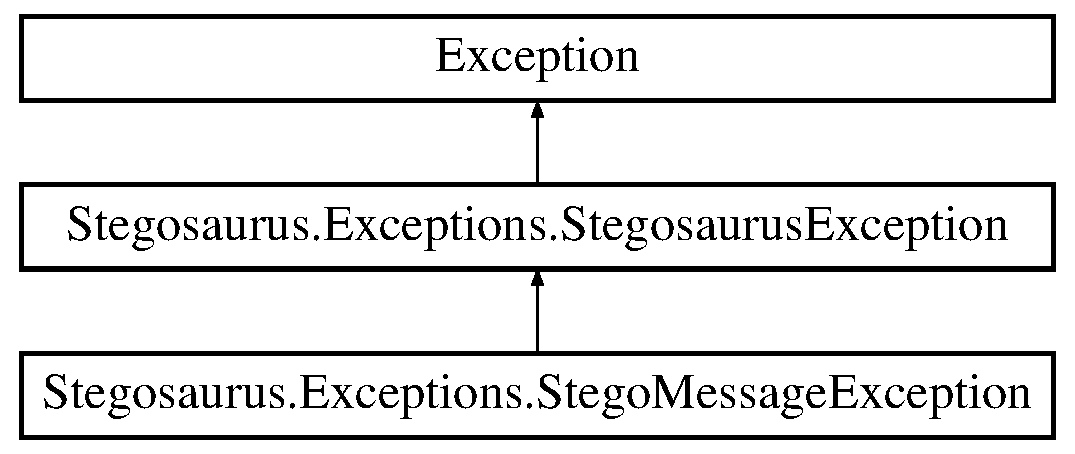
\includegraphics[height=3.000000cm]{class_stegosaurus_1_1_exceptions_1_1_stego_message_exception}
\end{center}
\end{figure}
\subsection*{Public Member Functions}
\begin{DoxyCompactItemize}
\item 
{\bfseries Stego\+Message\+Exception} (string message)\hypertarget{class_stegosaurus_1_1_exceptions_1_1_stego_message_exception_aed93bec652d63a8fa965f58be455db21}{}\label{class_stegosaurus_1_1_exceptions_1_1_stego_message_exception_aed93bec652d63a8fa965f58be455db21}

\item 
{\bfseries Stego\+Message\+Exception} (string message, Exception inner)\hypertarget{class_stegosaurus_1_1_exceptions_1_1_stego_message_exception_a8019781064571ac1df7cedc477415571}{}\label{class_stegosaurus_1_1_exceptions_1_1_stego_message_exception_a8019781064571ac1df7cedc477415571}

\end{DoxyCompactItemize}


The documentation for this class was generated from the following file\+:\begin{DoxyCompactItemize}
\item 
Steganography/\+Stegosaurus/\+Exceptions/Stego\+Message\+Exception.\+cs\end{DoxyCompactItemize}

\hypertarget{class_stegosaurus_1_1_exceptions_1_1_stegosaurus_exception}{}\section{Stegosaurus.\+Exceptions.\+Stegosaurus\+Exception Class Reference}
\label{class_stegosaurus_1_1_exceptions_1_1_stegosaurus_exception}\index{Stegosaurus.\+Exceptions.\+Stegosaurus\+Exception@{Stegosaurus.\+Exceptions.\+Stegosaurus\+Exception}}
Inheritance diagram for Stegosaurus.\+Exceptions.\+Stegosaurus\+Exception\+:\begin{figure}[H]
\begin{center}
\leavevmode
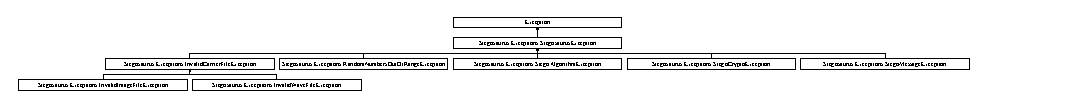
\includegraphics[height=0.985048cm]{class_stegosaurus_1_1_exceptions_1_1_stegosaurus_exception}
\end{center}
\end{figure}
\subsection*{Public Member Functions}
\begin{DoxyCompactItemize}
\item 
{\bfseries Stegosaurus\+Exception} (string message)\hypertarget{class_stegosaurus_1_1_exceptions_1_1_stegosaurus_exception_ab5364acb0e1e65fcd45458ee91f47ef9}{}\label{class_stegosaurus_1_1_exceptions_1_1_stegosaurus_exception_ab5364acb0e1e65fcd45458ee91f47ef9}

\item 
{\bfseries Stegosaurus\+Exception} (string message, Exception inner)\hypertarget{class_stegosaurus_1_1_exceptions_1_1_stegosaurus_exception_a8cccaf6c39b0b21a2fd12ce5c015991b}{}\label{class_stegosaurus_1_1_exceptions_1_1_stegosaurus_exception_a8cccaf6c39b0b21a2fd12ce5c015991b}

\end{DoxyCompactItemize}


The documentation for this class was generated from the following file\+:\begin{DoxyCompactItemize}
\item 
Steganography/\+Stegosaurus/\+Exceptions/Stegosaurus\+Exception.\+cs\end{DoxyCompactItemize}

\hypertarget{class_stegosaurus_1_1_cryptography_1_1_triple_d_e_s_provider}{}\section{Stegosaurus.\+Cryptography.\+Triple\+D\+E\+S\+Provider Class Reference}
\label{class_stegosaurus_1_1_cryptography_1_1_triple_d_e_s_provider}\index{Stegosaurus.\+Cryptography.\+Triple\+D\+E\+S\+Provider@{Stegosaurus.\+Cryptography.\+Triple\+D\+E\+S\+Provider}}
Inheritance diagram for Stegosaurus.\+Cryptography.\+Triple\+D\+E\+S\+Provider\+:\begin{figure}[H]
\begin{center}
\leavevmode
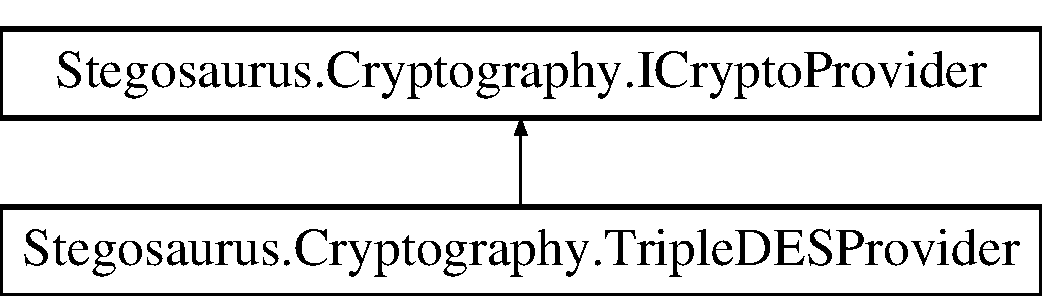
\includegraphics[height=2.000000cm]{class_stegosaurus_1_1_cryptography_1_1_triple_d_e_s_provider}
\end{center}
\end{figure}
\subsection*{Public Member Functions}
\begin{DoxyCompactItemize}
\item 
byte\mbox{[}$\,$\mbox{]} \hyperlink{class_stegosaurus_1_1_cryptography_1_1_triple_d_e_s_provider_aae9a3eb3f23e3c8995252d6f1184fd70}{Decrypt} (byte\mbox{[}$\,$\mbox{]} \+\_\+data)
\begin{DoxyCompactList}\small\item\em Decrypts and returns decrypted data. \end{DoxyCompactList}\item 
byte\mbox{[}$\,$\mbox{]} \hyperlink{class_stegosaurus_1_1_cryptography_1_1_triple_d_e_s_provider_a3af1ec710220cb696b1266d3317a4e79}{Encrypt} (byte\mbox{[}$\,$\mbox{]} \+\_\+data)
\begin{DoxyCompactList}\small\item\em Encrypts and returns encrypted data. \end{DoxyCompactList}\item 
byte\mbox{[}$\,$\mbox{]} \hyperlink{class_stegosaurus_1_1_cryptography_1_1_triple_d_e_s_provider_a7ed750ce72bf9adf2e35887d0ab67db8}{Generate\+Key} ()
\begin{DoxyCompactList}\small\item\em Generates and returns a key which can be used with the algorithm. \end{DoxyCompactList}\item 
void \hyperlink{class_stegosaurus_1_1_cryptography_1_1_triple_d_e_s_provider_ab7413df54e7753ae7ce4776f94521c7a}{Set\+Key} (string \+\_\+key\+String)
\begin{DoxyCompactList}\small\item\em Set the Key from a string. \end{DoxyCompactList}\end{DoxyCompactItemize}
\subsection*{Public Attributes}
\begin{DoxyCompactItemize}
\item 
string {\bfseries Name} =$>$ \char`\"{}Triple\+D\+ES\char`\"{}\hypertarget{class_stegosaurus_1_1_cryptography_1_1_triple_d_e_s_provider_a4ddc2254ae71540da33ef00ce4e49b8d}{}\label{class_stegosaurus_1_1_cryptography_1_1_triple_d_e_s_provider_a4ddc2254ae71540da33ef00ce4e49b8d}

\item 
int {\bfseries Seed} =$>$ Key == null ? 0 \+: Key.\+Compute\+Hash()\hypertarget{class_stegosaurus_1_1_cryptography_1_1_triple_d_e_s_provider_a427769de0c0cca31e102d8ba446fafc9}{}\label{class_stegosaurus_1_1_cryptography_1_1_triple_d_e_s_provider_a427769de0c0cca31e102d8ba446fafc9}

\item 
int {\bfseries Key\+Size} =$>$ 192\hypertarget{class_stegosaurus_1_1_cryptography_1_1_triple_d_e_s_provider_a5f69d616171d12dedc4f857d18183f0e}{}\label{class_stegosaurus_1_1_cryptography_1_1_triple_d_e_s_provider_a5f69d616171d12dedc4f857d18183f0e}

\end{DoxyCompactItemize}
\subsection*{Properties}
\begin{DoxyCompactItemize}
\item 
byte\mbox{[}$\,$\mbox{]} {\bfseries Key}\hspace{0.3cm}{\ttfamily  \mbox{[}get, set\mbox{]}}\hypertarget{class_stegosaurus_1_1_cryptography_1_1_triple_d_e_s_provider_af5d4438d8c3928502812e977d8c566ae}{}\label{class_stegosaurus_1_1_cryptography_1_1_triple_d_e_s_provider_af5d4438d8c3928502812e977d8c566ae}

\end{DoxyCompactItemize}


\subsection{Member Function Documentation}
\index{Stegosaurus\+::\+Cryptography\+::\+Triple\+D\+E\+S\+Provider@{Stegosaurus\+::\+Cryptography\+::\+Triple\+D\+E\+S\+Provider}!Decrypt@{Decrypt}}
\index{Decrypt@{Decrypt}!Stegosaurus\+::\+Cryptography\+::\+Triple\+D\+E\+S\+Provider@{Stegosaurus\+::\+Cryptography\+::\+Triple\+D\+E\+S\+Provider}}
\subsubsection[{\texorpdfstring{Decrypt(byte[] \+\_\+data)}{Decrypt(byte[] _data)}}]{\setlength{\rightskip}{0pt plus 5cm}byte \mbox{[}$\,$\mbox{]} Stegosaurus.\+Cryptography.\+Triple\+D\+E\+S\+Provider.\+Decrypt (
\begin{DoxyParamCaption}
\item[{byte\mbox{[}$\,$\mbox{]}}]{\+\_\+data}
\end{DoxyParamCaption}
)}\hypertarget{class_stegosaurus_1_1_cryptography_1_1_triple_d_e_s_provider_aae9a3eb3f23e3c8995252d6f1184fd70}{}\label{class_stegosaurus_1_1_cryptography_1_1_triple_d_e_s_provider_aae9a3eb3f23e3c8995252d6f1184fd70}


Decrypts and returns decrypted data. 



Implements \hyperlink{interface_stegosaurus_1_1_cryptography_1_1_i_crypto_provider_a673607b0f3392591db9c647d2499f38d}{Stegosaurus.\+Cryptography.\+I\+Crypto\+Provider}.

\index{Stegosaurus\+::\+Cryptography\+::\+Triple\+D\+E\+S\+Provider@{Stegosaurus\+::\+Cryptography\+::\+Triple\+D\+E\+S\+Provider}!Encrypt@{Encrypt}}
\index{Encrypt@{Encrypt}!Stegosaurus\+::\+Cryptography\+::\+Triple\+D\+E\+S\+Provider@{Stegosaurus\+::\+Cryptography\+::\+Triple\+D\+E\+S\+Provider}}
\subsubsection[{\texorpdfstring{Encrypt(byte[] \+\_\+data)}{Encrypt(byte[] _data)}}]{\setlength{\rightskip}{0pt plus 5cm}byte \mbox{[}$\,$\mbox{]} Stegosaurus.\+Cryptography.\+Triple\+D\+E\+S\+Provider.\+Encrypt (
\begin{DoxyParamCaption}
\item[{byte\mbox{[}$\,$\mbox{]}}]{\+\_\+data}
\end{DoxyParamCaption}
)}\hypertarget{class_stegosaurus_1_1_cryptography_1_1_triple_d_e_s_provider_a3af1ec710220cb696b1266d3317a4e79}{}\label{class_stegosaurus_1_1_cryptography_1_1_triple_d_e_s_provider_a3af1ec710220cb696b1266d3317a4e79}


Encrypts and returns encrypted data. 



Implements \hyperlink{interface_stegosaurus_1_1_cryptography_1_1_i_crypto_provider_a2222231bf16ba92e8efc8d515943aacd}{Stegosaurus.\+Cryptography.\+I\+Crypto\+Provider}.

\index{Stegosaurus\+::\+Cryptography\+::\+Triple\+D\+E\+S\+Provider@{Stegosaurus\+::\+Cryptography\+::\+Triple\+D\+E\+S\+Provider}!Generate\+Key@{Generate\+Key}}
\index{Generate\+Key@{Generate\+Key}!Stegosaurus\+::\+Cryptography\+::\+Triple\+D\+E\+S\+Provider@{Stegosaurus\+::\+Cryptography\+::\+Triple\+D\+E\+S\+Provider}}
\subsubsection[{\texorpdfstring{Generate\+Key()}{GenerateKey()}}]{\setlength{\rightskip}{0pt plus 5cm}byte \mbox{[}$\,$\mbox{]} Stegosaurus.\+Cryptography.\+Triple\+D\+E\+S\+Provider.\+Generate\+Key (
\begin{DoxyParamCaption}
{}
\end{DoxyParamCaption}
)}\hypertarget{class_stegosaurus_1_1_cryptography_1_1_triple_d_e_s_provider_a7ed750ce72bf9adf2e35887d0ab67db8}{}\label{class_stegosaurus_1_1_cryptography_1_1_triple_d_e_s_provider_a7ed750ce72bf9adf2e35887d0ab67db8}


Generates and returns a key which can be used with the algorithm. 



Implements \hyperlink{interface_stegosaurus_1_1_cryptography_1_1_i_crypto_provider_ae25c64411409f0cc41c2282030c6dc5c}{Stegosaurus.\+Cryptography.\+I\+Crypto\+Provider}.

\index{Stegosaurus\+::\+Cryptography\+::\+Triple\+D\+E\+S\+Provider@{Stegosaurus\+::\+Cryptography\+::\+Triple\+D\+E\+S\+Provider}!Set\+Key@{Set\+Key}}
\index{Set\+Key@{Set\+Key}!Stegosaurus\+::\+Cryptography\+::\+Triple\+D\+E\+S\+Provider@{Stegosaurus\+::\+Cryptography\+::\+Triple\+D\+E\+S\+Provider}}
\subsubsection[{\texorpdfstring{Set\+Key(string \+\_\+key\+String)}{SetKey(string _keyString)}}]{\setlength{\rightskip}{0pt plus 5cm}void Stegosaurus.\+Cryptography.\+Triple\+D\+E\+S\+Provider.\+Set\+Key (
\begin{DoxyParamCaption}
\item[{string}]{\+\_\+key\+String}
\end{DoxyParamCaption}
)}\hypertarget{class_stegosaurus_1_1_cryptography_1_1_triple_d_e_s_provider_ab7413df54e7753ae7ce4776f94521c7a}{}\label{class_stegosaurus_1_1_cryptography_1_1_triple_d_e_s_provider_ab7413df54e7753ae7ce4776f94521c7a}


Set the Key from a string. 



Implements \hyperlink{interface_stegosaurus_1_1_cryptography_1_1_i_crypto_provider_a95c1bb37e8bfdb62e6f66e8094d9d51b}{Stegosaurus.\+Cryptography.\+I\+Crypto\+Provider}.



The documentation for this class was generated from the following file\+:\begin{DoxyCompactItemize}
\item 
Steganography/\+Stegosaurus/\+Cryptography/Triple\+D\+E\+S\+Provider.\+cs\end{DoxyCompactItemize}

\hypertarget{class_stegosaurus_1_1_algorithm_1_1_graph_theory_1_1_vertex}{}\section{Stegosaurus.\+Algorithm.\+Graph\+Theory.\+Vertex Class Reference}
\label{class_stegosaurus_1_1_algorithm_1_1_graph_theory_1_1_vertex}\index{Stegosaurus.\+Algorithm.\+Graph\+Theory.\+Vertex@{Stegosaurus.\+Algorithm.\+Graph\+Theory.\+Vertex}}
\subsection*{Public Member Functions}
\begin{DoxyCompactItemize}
\item 
{\bfseries Vertex} (\hyperlink{class_stegosaurus_1_1_algorithm_1_1_graph_theory_1_1_sample}{Sample}\mbox{[}$\,$\mbox{]} \+\_\+samples)\hypertarget{class_stegosaurus_1_1_algorithm_1_1_graph_theory_1_1_vertex_a9441081614ef3fbf3f8baf25de92533e}{}\label{class_stegosaurus_1_1_algorithm_1_1_graph_theory_1_1_vertex_a9441081614ef3fbf3f8baf25de92533e}

\item 
override string {\bfseries To\+String} ()\hypertarget{class_stegosaurus_1_1_algorithm_1_1_graph_theory_1_1_vertex_aede634e13ec0c349ff353b95fa12c86e}{}\label{class_stegosaurus_1_1_algorithm_1_1_graph_theory_1_1_vertex_aede634e13ec0c349ff353b95fa12c86e}

\end{DoxyCompactItemize}
\subsection*{Public Attributes}
\begin{DoxyCompactItemize}
\item 
\hyperlink{class_stegosaurus_1_1_algorithm_1_1_graph_theory_1_1_sample}{Sample}\mbox{[}$\,$\mbox{]} {\bfseries Samples}\hypertarget{class_stegosaurus_1_1_algorithm_1_1_graph_theory_1_1_vertex_a3254f850d0ce3fee41f27259e41ce31f}{}\label{class_stegosaurus_1_1_algorithm_1_1_graph_theory_1_1_vertex_a3254f850d0ce3fee41f27259e41ce31f}

\item 
List$<$ \hyperlink{class_stegosaurus_1_1_algorithm_1_1_graph_theory_1_1_edge}{Edge} $>$ {\bfseries Edges} = new List$<$\hyperlink{class_stegosaurus_1_1_algorithm_1_1_graph_theory_1_1_edge}{Edge}$>$()\hypertarget{class_stegosaurus_1_1_algorithm_1_1_graph_theory_1_1_vertex_a22f4be1090f0acf10ffb15d6c5d7a0b8}{}\label{class_stegosaurus_1_1_algorithm_1_1_graph_theory_1_1_vertex_a22f4be1090f0acf10ffb15d6c5d7a0b8}

\item 
short {\bfseries Value}\hypertarget{class_stegosaurus_1_1_algorithm_1_1_graph_theory_1_1_vertex_a935733b0ab048d9bc810ec9669905b06}{}\label{class_stegosaurus_1_1_algorithm_1_1_graph_theory_1_1_vertex_a935733b0ab048d9bc810ec9669905b06}

\item 
short {\bfseries Value\+Dif}\hypertarget{class_stegosaurus_1_1_algorithm_1_1_graph_theory_1_1_vertex_a56d8f272df5763992eb49d46bac8d436}{}\label{class_stegosaurus_1_1_algorithm_1_1_graph_theory_1_1_vertex_a56d8f272df5763992eb49d46bac8d436}

\item 
int {\bfseries num\+Edges} = 0\hypertarget{class_stegosaurus_1_1_algorithm_1_1_graph_theory_1_1_vertex_a0586048bb0cc119ff03943d77a71a187}{}\label{class_stegosaurus_1_1_algorithm_1_1_graph_theory_1_1_vertex_a0586048bb0cc119ff03943d77a71a187}

\item 
bool {\bfseries Is\+Valid}\hypertarget{class_stegosaurus_1_1_algorithm_1_1_graph_theory_1_1_vertex_a76da4ccf338f716af354c9f31856c222}{}\label{class_stegosaurus_1_1_algorithm_1_1_graph_theory_1_1_vertex_a76da4ccf338f716af354c9f31856c222}

\end{DoxyCompactItemize}


The documentation for this class was generated from the following file\+:\begin{DoxyCompactItemize}
\item 
Steganography/\+Stegosaurus/\+Algorithm/\+Graph\+Theory/Vertex.\+cs\end{DoxyCompactItemize}

\hypertarget{class_stegosaurus_1_1_carrier_1_1_audio_formats_1_1_wave_file}{}\section{Stegosaurus.\+Carrier.\+Audio\+Formats.\+Wave\+File Class Reference}
\label{class_stegosaurus_1_1_carrier_1_1_audio_formats_1_1_wave_file}\index{Stegosaurus.\+Carrier.\+Audio\+Formats.\+Wave\+File@{Stegosaurus.\+Carrier.\+Audio\+Formats.\+Wave\+File}}
Inheritance diagram for Stegosaurus.\+Carrier.\+Audio\+Formats.\+Wave\+File\+:\begin{figure}[H]
\begin{center}
\leavevmode
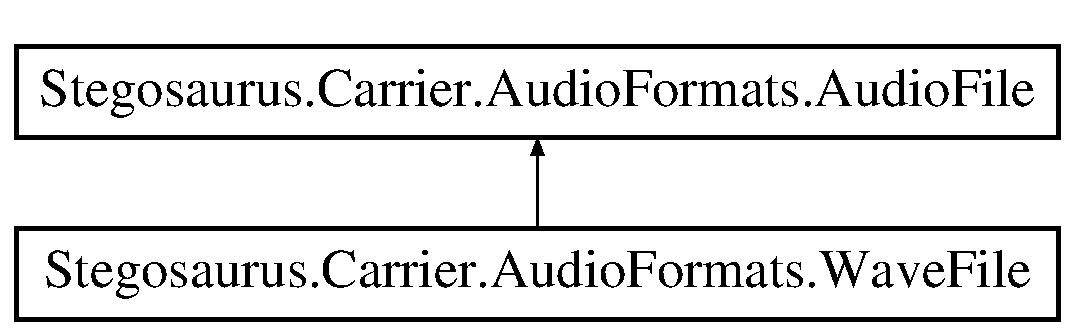
\includegraphics[height=2.000000cm]{class_stegosaurus_1_1_carrier_1_1_audio_formats_1_1_wave_file}
\end{center}
\end{figure}
\subsection*{Public Member Functions}
\begin{DoxyCompactItemize}
\item 
\hyperlink{class_stegosaurus_1_1_carrier_1_1_audio_formats_1_1_wave_file_acab11a7e34412f40fbe7da33d7debd65}{Wave\+File} (string \+\_\+file\+Path)
\begin{DoxyCompactList}\small\item\em Construct a \hyperlink{class_stegosaurus_1_1_carrier_1_1_audio_formats_1_1_wave_file}{Wave\+File} from a file path. \end{DoxyCompactList}\item 
override void \hyperlink{class_stegosaurus_1_1_carrier_1_1_audio_formats_1_1_wave_file_aa18e174d66b4d3fefef8683b35946120}{Parse} (string \+\_\+file\+Path)
\begin{DoxyCompactList}\small\item\em Parses an audio file by reading its headers and samples. \end{DoxyCompactList}\item 
override byte\mbox{[}$\,$\mbox{]} \hyperlink{class_stegosaurus_1_1_carrier_1_1_audio_formats_1_1_wave_file_a3de2c6ede07d46d1bfc3082fcf07d015}{To\+Array} ()
\begin{DoxyCompactList}\small\item\em Reconstructs and returns the entire byte array of the file, including headers. \end{DoxyCompactList}\end{DoxyCompactItemize}
\subsection*{Properties}
\begin{DoxyCompactItemize}
\item 
int \hyperlink{class_stegosaurus_1_1_carrier_1_1_audio_formats_1_1_wave_file_a65d3fa2945c148a89857b8fdf0612e7d}{Chunk\+Size}\hspace{0.3cm}{\ttfamily  \mbox{[}get\mbox{]}}
\begin{DoxyCompactList}\small\item\em Get or set the chunk size. \end{DoxyCompactList}\item 
int \hyperlink{class_stegosaurus_1_1_carrier_1_1_audio_formats_1_1_wave_file_a5981b47062913ff15855b36e4c20ff7c}{Format\+Sub\+Chunk\+Size}\hspace{0.3cm}{\ttfamily  \mbox{[}get\mbox{]}}
\begin{DoxyCompactList}\small\item\em Get or set the size of the format subchunk. \end{DoxyCompactList}\item 
int \hyperlink{class_stegosaurus_1_1_carrier_1_1_audio_formats_1_1_wave_file_a9f9e6f23de0403b656c4cc337def8f49}{Data\+Sub\+Chunk\+Size}\hspace{0.3cm}{\ttfamily  \mbox{[}get\mbox{]}}
\begin{DoxyCompactList}\small\item\em Get or set the size of the data subchunk. \end{DoxyCompactList}\item 
short \hyperlink{class_stegosaurus_1_1_carrier_1_1_audio_formats_1_1_wave_file_a9e8c8db340f18d23110b9711c9134531}{Audio\+Format}\hspace{0.3cm}{\ttfamily  \mbox{[}get\mbox{]}}
\begin{DoxyCompactList}\small\item\em Get or set the audio format. \end{DoxyCompactList}\end{DoxyCompactItemize}
\subsection*{Additional Inherited Members}


\subsection{Constructor \& Destructor Documentation}
\index{Stegosaurus\+::\+Carrier\+::\+Audio\+Formats\+::\+Wave\+File@{Stegosaurus\+::\+Carrier\+::\+Audio\+Formats\+::\+Wave\+File}!Wave\+File@{Wave\+File}}
\index{Wave\+File@{Wave\+File}!Stegosaurus\+::\+Carrier\+::\+Audio\+Formats\+::\+Wave\+File@{Stegosaurus\+::\+Carrier\+::\+Audio\+Formats\+::\+Wave\+File}}
\subsubsection[{\texorpdfstring{Wave\+File(string \+\_\+file\+Path)}{WaveFile(string _filePath)}}]{\setlength{\rightskip}{0pt plus 5cm}Stegosaurus.\+Carrier.\+Audio\+Formats.\+Wave\+File.\+Wave\+File (
\begin{DoxyParamCaption}
\item[{string}]{\+\_\+file\+Path}
\end{DoxyParamCaption}
)}\hypertarget{class_stegosaurus_1_1_carrier_1_1_audio_formats_1_1_wave_file_acab11a7e34412f40fbe7da33d7debd65}{}\label{class_stegosaurus_1_1_carrier_1_1_audio_formats_1_1_wave_file_acab11a7e34412f40fbe7da33d7debd65}


Construct a \hyperlink{class_stegosaurus_1_1_carrier_1_1_audio_formats_1_1_wave_file}{Wave\+File} from a file path. 



\subsection{Member Function Documentation}
\index{Stegosaurus\+::\+Carrier\+::\+Audio\+Formats\+::\+Wave\+File@{Stegosaurus\+::\+Carrier\+::\+Audio\+Formats\+::\+Wave\+File}!Parse@{Parse}}
\index{Parse@{Parse}!Stegosaurus\+::\+Carrier\+::\+Audio\+Formats\+::\+Wave\+File@{Stegosaurus\+::\+Carrier\+::\+Audio\+Formats\+::\+Wave\+File}}
\subsubsection[{\texorpdfstring{Parse(string \+\_\+file\+Path)}{Parse(string _filePath)}}]{\setlength{\rightskip}{0pt plus 5cm}override void Stegosaurus.\+Carrier.\+Audio\+Formats.\+Wave\+File.\+Parse (
\begin{DoxyParamCaption}
\item[{string}]{\+\_\+file\+Path}
\end{DoxyParamCaption}
)\hspace{0.3cm}{\ttfamily [virtual]}}\hypertarget{class_stegosaurus_1_1_carrier_1_1_audio_formats_1_1_wave_file_aa18e174d66b4d3fefef8683b35946120}{}\label{class_stegosaurus_1_1_carrier_1_1_audio_formats_1_1_wave_file_aa18e174d66b4d3fefef8683b35946120}


Parses an audio file by reading its headers and samples. 



Implements \hyperlink{class_stegosaurus_1_1_carrier_1_1_audio_formats_1_1_audio_file_a52a9349e3c5cf18eca6f61cee8d81d2b}{Stegosaurus.\+Carrier.\+Audio\+Formats.\+Audio\+File}.

\index{Stegosaurus\+::\+Carrier\+::\+Audio\+Formats\+::\+Wave\+File@{Stegosaurus\+::\+Carrier\+::\+Audio\+Formats\+::\+Wave\+File}!To\+Array@{To\+Array}}
\index{To\+Array@{To\+Array}!Stegosaurus\+::\+Carrier\+::\+Audio\+Formats\+::\+Wave\+File@{Stegosaurus\+::\+Carrier\+::\+Audio\+Formats\+::\+Wave\+File}}
\subsubsection[{\texorpdfstring{To\+Array()}{ToArray()}}]{\setlength{\rightskip}{0pt plus 5cm}override byte \mbox{[}$\,$\mbox{]} Stegosaurus.\+Carrier.\+Audio\+Formats.\+Wave\+File.\+To\+Array (
\begin{DoxyParamCaption}
{}
\end{DoxyParamCaption}
)\hspace{0.3cm}{\ttfamily [virtual]}}\hypertarget{class_stegosaurus_1_1_carrier_1_1_audio_formats_1_1_wave_file_a3de2c6ede07d46d1bfc3082fcf07d015}{}\label{class_stegosaurus_1_1_carrier_1_1_audio_formats_1_1_wave_file_a3de2c6ede07d46d1bfc3082fcf07d015}


Reconstructs and returns the entire byte array of the file, including headers. 



Implements \hyperlink{class_stegosaurus_1_1_carrier_1_1_audio_formats_1_1_audio_file_ac62f509a70ce93baab9b8112198ff6ac}{Stegosaurus.\+Carrier.\+Audio\+Formats.\+Audio\+File}.



\subsection{Property Documentation}
\index{Stegosaurus\+::\+Carrier\+::\+Audio\+Formats\+::\+Wave\+File@{Stegosaurus\+::\+Carrier\+::\+Audio\+Formats\+::\+Wave\+File}!Audio\+Format@{Audio\+Format}}
\index{Audio\+Format@{Audio\+Format}!Stegosaurus\+::\+Carrier\+::\+Audio\+Formats\+::\+Wave\+File@{Stegosaurus\+::\+Carrier\+::\+Audio\+Formats\+::\+Wave\+File}}
\subsubsection[{\texorpdfstring{Audio\+Format}{AudioFormat}}]{\setlength{\rightskip}{0pt plus 5cm}short Stegosaurus.\+Carrier.\+Audio\+Formats.\+Wave\+File.\+Audio\+Format\hspace{0.3cm}{\ttfamily [get]}}\hypertarget{class_stegosaurus_1_1_carrier_1_1_audio_formats_1_1_wave_file_a9e8c8db340f18d23110b9711c9134531}{}\label{class_stegosaurus_1_1_carrier_1_1_audio_formats_1_1_wave_file_a9e8c8db340f18d23110b9711c9134531}


Get or set the audio format. 

\index{Stegosaurus\+::\+Carrier\+::\+Audio\+Formats\+::\+Wave\+File@{Stegosaurus\+::\+Carrier\+::\+Audio\+Formats\+::\+Wave\+File}!Chunk\+Size@{Chunk\+Size}}
\index{Chunk\+Size@{Chunk\+Size}!Stegosaurus\+::\+Carrier\+::\+Audio\+Formats\+::\+Wave\+File@{Stegosaurus\+::\+Carrier\+::\+Audio\+Formats\+::\+Wave\+File}}
\subsubsection[{\texorpdfstring{Chunk\+Size}{ChunkSize}}]{\setlength{\rightskip}{0pt plus 5cm}int Stegosaurus.\+Carrier.\+Audio\+Formats.\+Wave\+File.\+Chunk\+Size\hspace{0.3cm}{\ttfamily [get]}}\hypertarget{class_stegosaurus_1_1_carrier_1_1_audio_formats_1_1_wave_file_a65d3fa2945c148a89857b8fdf0612e7d}{}\label{class_stegosaurus_1_1_carrier_1_1_audio_formats_1_1_wave_file_a65d3fa2945c148a89857b8fdf0612e7d}


Get or set the chunk size. 

\index{Stegosaurus\+::\+Carrier\+::\+Audio\+Formats\+::\+Wave\+File@{Stegosaurus\+::\+Carrier\+::\+Audio\+Formats\+::\+Wave\+File}!Data\+Sub\+Chunk\+Size@{Data\+Sub\+Chunk\+Size}}
\index{Data\+Sub\+Chunk\+Size@{Data\+Sub\+Chunk\+Size}!Stegosaurus\+::\+Carrier\+::\+Audio\+Formats\+::\+Wave\+File@{Stegosaurus\+::\+Carrier\+::\+Audio\+Formats\+::\+Wave\+File}}
\subsubsection[{\texorpdfstring{Data\+Sub\+Chunk\+Size}{DataSubChunkSize}}]{\setlength{\rightskip}{0pt plus 5cm}int Stegosaurus.\+Carrier.\+Audio\+Formats.\+Wave\+File.\+Data\+Sub\+Chunk\+Size\hspace{0.3cm}{\ttfamily [get]}}\hypertarget{class_stegosaurus_1_1_carrier_1_1_audio_formats_1_1_wave_file_a9f9e6f23de0403b656c4cc337def8f49}{}\label{class_stegosaurus_1_1_carrier_1_1_audio_formats_1_1_wave_file_a9f9e6f23de0403b656c4cc337def8f49}


Get or set the size of the data subchunk. 

\index{Stegosaurus\+::\+Carrier\+::\+Audio\+Formats\+::\+Wave\+File@{Stegosaurus\+::\+Carrier\+::\+Audio\+Formats\+::\+Wave\+File}!Format\+Sub\+Chunk\+Size@{Format\+Sub\+Chunk\+Size}}
\index{Format\+Sub\+Chunk\+Size@{Format\+Sub\+Chunk\+Size}!Stegosaurus\+::\+Carrier\+::\+Audio\+Formats\+::\+Wave\+File@{Stegosaurus\+::\+Carrier\+::\+Audio\+Formats\+::\+Wave\+File}}
\subsubsection[{\texorpdfstring{Format\+Sub\+Chunk\+Size}{FormatSubChunkSize}}]{\setlength{\rightskip}{0pt plus 5cm}int Stegosaurus.\+Carrier.\+Audio\+Formats.\+Wave\+File.\+Format\+Sub\+Chunk\+Size\hspace{0.3cm}{\ttfamily [get]}}\hypertarget{class_stegosaurus_1_1_carrier_1_1_audio_formats_1_1_wave_file_a5981b47062913ff15855b36e4c20ff7c}{}\label{class_stegosaurus_1_1_carrier_1_1_audio_formats_1_1_wave_file_a5981b47062913ff15855b36e4c20ff7c}


Get or set the size of the format subchunk. 



The documentation for this class was generated from the following file\+:\begin{DoxyCompactItemize}
\item 
Steganography/\+Stegosaurus/\+Carrier/\+Audio\+Formats/Wave\+File.\+cs\end{DoxyCompactItemize}

%--- End generated contents ---

% Index
\backmatter
\newpage
\phantomsection
\clearemptydoublepage
\addcontentsline{toc}{chapter}{Index}
\printindex

\end{document}
